% !TeX program = xelatex
% (C) Hans Wan, Windy Deng
% Licensed under CC BY-NC-SA 4.0 International license.
% This is the LaTeX source code of Your Missing Semester of Using Computer (PDF Version).

\documentclass[a4paper]{book}
\usepackage{missing}

\date{\today}

\begin{document}

\pagenumbering{Alph}
\maketitle

\frontmatter
\pdfbookmark{内封}{innertitle}
\thispagestyle{empty}
\begin{center}
  \vspace*{2.5cm}
  \fontsize{42pt}{54pt}\selectfont{}\textsf{你缺失的那门}\par
  \fontsize{18pt}{18pt}\selectfont{}\textsf{Your Missing Semester of Using Computer}\par
  \fontsize{54pt}{8pt}\selectfont{}\textbf{\textsf{计算机课}}\par
  \vspace*{3.6cm}
\end{center}

\begin{note}
  本教程在持续更新之中,因此十分期望得到读者的建议和意见。
  无论是对编写方向有好的建议,还是发现了叙述不正确或不严谨的地方,亦或是找到了一个错别字,都请将反馈发送到邮箱 \href{mailto:missing@criwits.top}{missing@criwits.top}。
\end{note}

这是一份适合「电脑小白」的电脑使用技巧手册。
它以近乎「手把手教」的语言,介绍了从基本的文件管理到软件的寻找安装,从简要的硬件组成到电脑的安全防护,从小的使用技巧到优良软件推荐的许多内容,旨在帮助对电脑操作不甚了解的所谓「小白」逐渐上手电脑的使用。

\begin{center}
  \vspace*{1cm}
  
\includegraphics[width=5cm]{assets/QR_CODE.png}\par
  访问 \url{https://missing.criwits.top/} 或扫码阅读本教程的最新版本!\par
\end{center}  

\tableofcontents

\chapter{序}
\label{premble}

按理来说,对于所谓「Z 世代」的年轻人,熟练地使用电脑应该是他们的生活必备技能。

但事实却出乎我们意料。据我们观察,许多同学对电脑的使用也并不熟悉,甚至可以说是陌生:
他们可能在网上被下载到各种「P2P 高速下载器」,面对着满电脑的流氓软件而不知所措;
他们可能对着别人发来的 \texttt{zip} 或 \texttt{7z} 文件一头雾水,对「压缩」和「解压缩」都不甚熟悉;
他们可能装着四五个浏览器、三四个杀毒软件,更可能分不清自己电脑的「内存」和「硬盘」……

有人说,这是由于智能手机的普及造成的。
显然,使用电脑与使用手机相比,「复杂」了不止一个数量级;而随着智能手机的不断发展,人们借助一部手机就能完成许多事情,电脑似乎已经不再需要了。
可是,尽管几年前就有人说「电脑现在已经是夕阳产业了」,但事实却是:
至少在当下,我们仍然得学会去用电脑,不说多么「精通」,但至少要能知道「软件怎么找怎么装」「出现小问题怎么办」「XX 文件怎么打开」「怎么把文件打包」等等这些「21 世纪的常识」。

中小学的《信息技术》课堂、大学的《大学计算机基础》课程本应起到教授这些知识的作用。
可惜,事与愿违——很多时候,我们在这些课堂上学到的东西,可能一辈子都用不到;真正需要学的东西,却缺失了:

我们一辈子可能也不会再尝试用 Excel 排出张三李四不及格的科目有哪些,不会再折腾复杂到毫无意义的页眉和页脚,不会再碰和动画制作和网页相关的任何内容。
但我们未来必然有无数次会需要去网上下载一个新的软件,会无数次遇到各种各样的软件错误、闪退或者崩溃,会无数次因为 Windows 更新导致这样或那样的问题,会无数次遇到电脑沾上垃圾软件而奇慢无比无法使用……

这份《Your Missing Semester of Using Computer》是一份为「电脑小白」准备的电脑操作指南。
它直译过来就是《你缺失的那门计算机课》,也可以叫做《你本应学过的计算机课》。
我们会假定读者基本不了解电脑的操作,换言之就是所谓「电脑小白」,告诉读者「电脑最好怎么用」。

这份教程会在文中简称自己为《Missing》。
《Missing》的得名参考了 MIT 的《\href{https://missing.csail.mit.edu/}{The Missing Semester of Your CS Education}》。

\mainmatter

\part{基础篇}
\addtocontents{toc}{\protect\footnotetext[2]{标有「*」的为选读内容}}

\setcounter{chapter}{-1}

\chapter{一些约定与预备知识}
\label{cha:first-things-first}

俗话说,「磨刀不误砍柴工」。在一切开始之前,我们先对本书中的一些标记和约定进行说明,同时为你提供一些可能有助于你更好地阅读本书的预备知识。

\section{《你缺计课》是什么}

《你缺计课》是一门\regcolor{面向当下的「零门槛」电脑课}:《你缺计课》旨在帮助你轻松掌握「如何在当下更高效地使用电脑」。如果你是电脑小白,本书会手把手地引导你迈入数字世界;如果你已经熟悉电脑操作,它也能助你发现可能忽略的小技巧,查漏补缺。

《你缺计课》是一本\regcolor{展望未来的「信息化」科普书}:从计算技术到人工智能,从云计算到网络安全,本书以通俗易懂的语言,带你探索这些塑造当今与未来的核心技术,让你对信息化世界有更清晰的认识。

\section{《你缺计课》不是什么}

《你缺计课》\regcolor{不是任何软件的使用手册}:本书不会详细讲解某款软件的具体操作方法。相反,我们更注重帮助你理解各种软件的功能、特点以及它们在不同场景中的作用。

《你缺计课》\regcolor{不是大部头而死板的教材}:有别于枯燥、繁琐而呆板的专业教材,本书希望和你成为朋友,与你一同踏上一场轻松愉快的旅程。它轻松、有趣、接地气,贴近生活,伴你前行。

\section{文中的标记符号}

\begin{wrapfigure}[5]{r}{2.5cm}
  \centering
  \vspace*{-1ex}
  
\includegraphics[width=2cm]{assets/basic/This_PC.png}
  % \caption{一些文件}
  % \label{fig:5_files}
\end{wrapfigure}

在《你缺计课》中,我们使用方头括号「【】」来标记所有屏幕上字面显示的选项。例如,当我们希望你右键桌面上长得右图一样的图标时,我们会称「右键【此电脑】」。

% \begin{figure}[htb!]
%   \centering
%   
\includegraphics[width=2cm]{assets/basic/This_PC.png}
% \end{figure}

我们使用右箭头「→」来表示下一步操作。例如,「右键【此电脑】→【属性】」的意思是,右键桌面上的【此电脑】图标,然后在弹出的菜单中点击【属性】。

如果某一章节的标题后带有星号「*」,表明这一章节内容可能较难理解,可以选择性阅读。

本书中的网页链接与邮箱地址会以这种样式呈现:\url{https://criwits.top/missing};一些代码片段、文件路径、特殊数字等内容会以 \MissingVerb{这种形式} 呈现。

\begin{note}
  有这种特殊外框的文字,通常是一些题外话。它们可能是一些供你思考的问题,或是一些有助于理解正文的额外知识。
\end{note}

\begin{MissingVerbatim}
这种特殊外框的文字是上述“代码片段”等内容的“升级版”,在内容太长,行内空间不足以展示时使用。这种环境包含的内容不能随意换行,过长的一行文字会用假换行标记标出,比如这行,看起来有三行,其实是一行。
这才是第二行。
\end{MissingVerbatim}

\section{《你缺计课》适合我的电脑吗?}

《你缺计课》适合所有使用 Windows 11 或 Windows 10 操作系统的电脑,书中所有操作均基于它们的简体中文版描述。如果你使用的是 Windows 11 或者 Windows 10,那么《你缺计课》非常适合你!

上一代的 Windows 版本,比如 Windows 7 或 Windows 8.1,在部分操作的细节上与 Windows 11 和 Windows 10 有不同——例如,在 Windows 7 中,修改系统设置要前往「控制面板」而非「设置」app。如果你使用的是这些早期 Windows 版本,你依然可以运用本书学习大量的通用知识,但在涉及具体操作时,你可能需要查阅其他资料。

如果你在使用非 Windows 的操作系统,比如苹果电脑上的 macOS、华为的「鸿蒙」系统或是各种 Linux 发行版,本书介绍的所有操作都可能不再适用。不过,本书介绍的大量通用的计算机科学知识——从\hyperref[cha:computer-and-its-components]{\CJKunderwave{电脑硬件的组成}},到「\hyperref[cha:file-and-file-management]{\CJKunderwave{文件}}」「\hyperref[cha:archive-formats-and-tools]{\CJKunderwave{压缩}}」等概念,以及\hyperref[cha:browsers-and-how-to-choose]{\CJKunderwave{浏览器}}、\hyperref[cha:mail-and-instant-messaging]{\CJKunderwave{即时通信工具}}、\hyperref[cha:office-and-wps]{\CJKunderwave{办公软件}}之间的相互比较,再到 \hyperref[cha:bring-intelligence-to-machines]{\CJKunderwave{人工智能}}、\hyperref[cha:introduction-to-cryptology]{\CJKunderwave{密码学}}和\hyperref[cha:cloud-computing-and-iot]{\CJKunderwave{云计算}}这些前沿话题——并不局限于某一特定的操作系统。你可以将本书作为一本科普读物,尽管它无法指导你具体的电脑操作,但仍然可以教给你许多知识。

不知道什么是「操作系统」?请参阅\chapref{cha:computer-and-its-components}。

\section{最最基础的预备知识}

虽然《你缺计课》自称「『零门槛』电脑课」,但我们还是希望读者有按过几下键盘、点过几下鼠标的经验。我们不会一个个按钮地告诉各位怎么去点,也不会一块块区域地告诉各位它在哪里,如果有些基本术语你不甚了解,下面的示意图可能会有所帮助。

\begin{figure}[htb!]
  \centering
  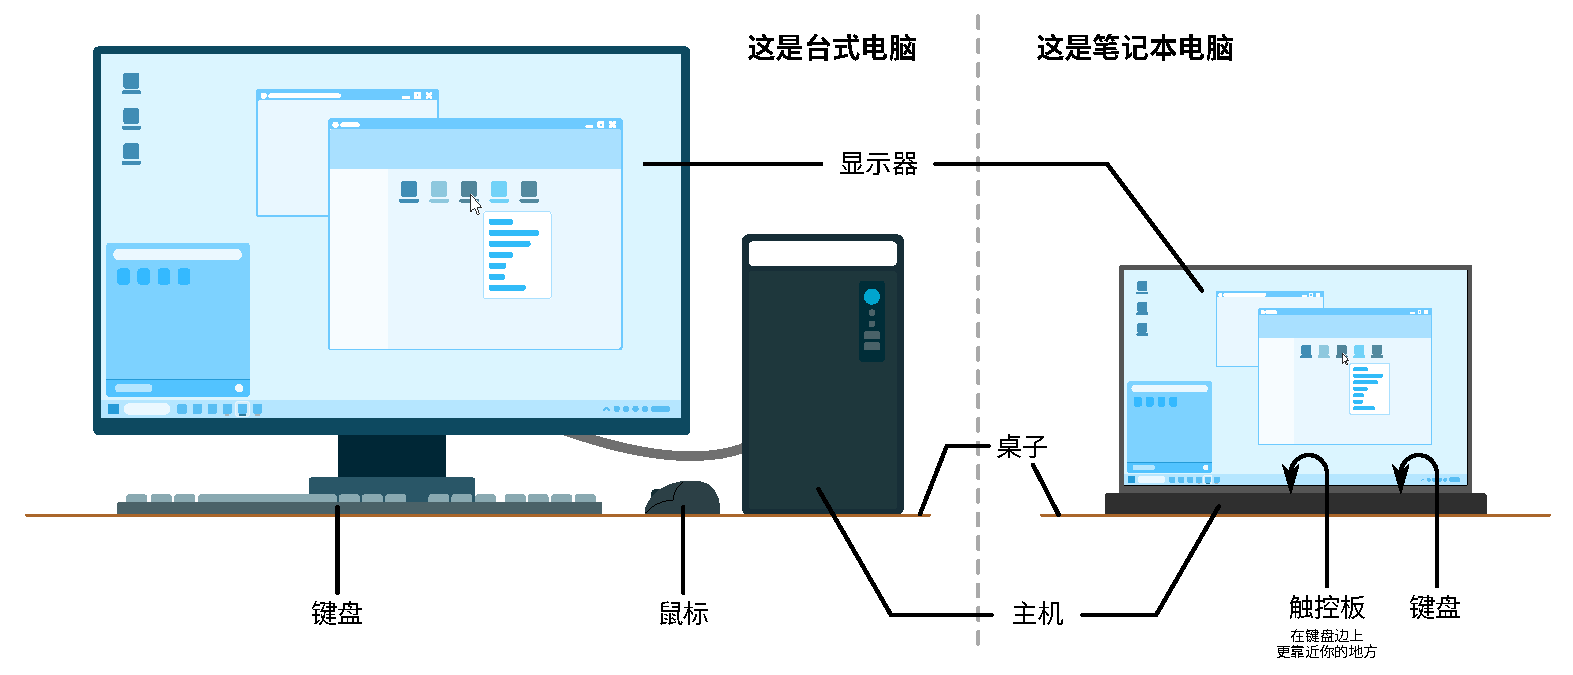
\includegraphics[width=.85\textwidth]{assets/basic/Simple_Computer.pdf}
  \caption{电脑各部分的结构}
  \label{fig:Simple_Computer}
\end{figure}

\begin{figure}[htb!]
  \centering
  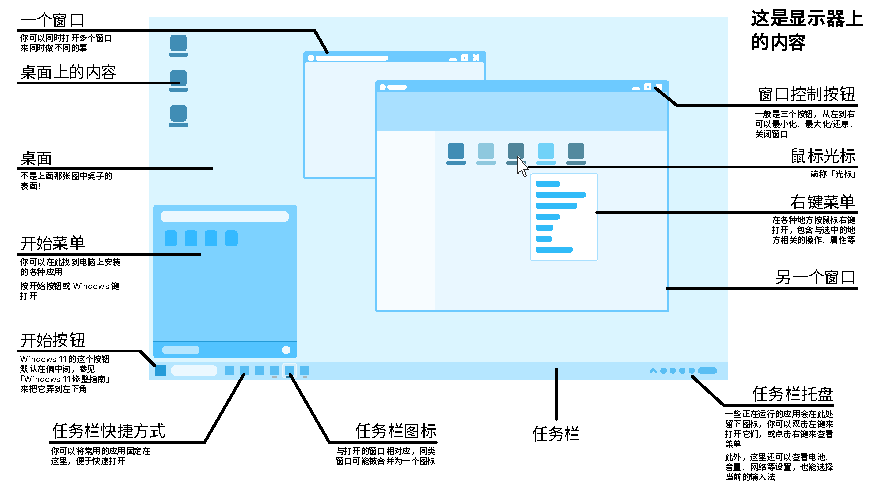
\includegraphics[width=.85\textwidth]{assets/basic/Simple_Windows.pdf}
  \caption{Windows 的基本组件}
  \label{fig:Simple_Windows}
\end{figure}

\section{快捷键的操作说明}

如果你按快捷键(组合键)后,电脑并没有行使预想的功能,可能是你的按法不对。快捷键的按法并不是「同时按下所有的键」,而是「依展示次序按下各键不松手,最后一起松开」。例如,若要按快捷键「\keys{\Windows + Shift + S}」:

\begin{itemize}
  \item 先按住 \keys{\Windows} 键(\keys{\Windows} 键上印有 Windows 徽标「\Windows」或「\WindowsTen」,一般来说这个键在 \keys{Ctrl} 和 \keys{Alt} 之间)不要松手;
  \item 再按住 \keys{Shift} 键,同样不要松手;
  \item 接着按一下 \keys{S} 键,然后松开全部按键。
\end{itemize}

\section{\keys{F1} -- \keys{F12} 功能键的使用说明}

在很久以前,人们为了增加电脑键盘的使用效率,在键盘的最顶端设计了一排按键,它们就是 \keys{F1} -- \keys{F12} 功能键。这些功能键和键盘上的 \keys{Ctrl}、\keys{Alt} 等键一样,并不能用来输入文字,而是用来组合出各种功能的。比如,\keys{Alt + F4} 可以用来关闭当前程序,\keys{F5} 可以用来刷新网页,\keys{F1} 用来查找帮助等。

随着电脑操作方式不断演进,\keys{F1} -- \keys{F12} 键使用得越来越少。这时,人们想,与其让这些键在键盘上吃灰,不如赋予它们一些新功能,比如快捷调整屏幕亮度、音量、无线网络连接等设置。于是,一些电脑键盘,尤其是笔记本电脑的键盘上,这 12 个按键在它们原本的功能之外,增加了一层「扩展功能」。

\begin{figure}[htb!]
  \centering
  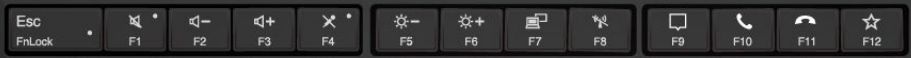
\includegraphics[width=.9\textwidth]{assets/basic/F1_to_F12_keys_with_extra_functions.png}
  \caption{带有额外功能的 F1—F12 功能键}
  \label{fig:F1_to_F12_keys_with_extra_functions}
\end{figure}

上图展示的就是 \keys{F1} -- \keys{F12} 键拥有扩展功能的键盘。这里,\keys{F1} -- \keys{F12} 这些键上被画上了一些符号。这些符号代表了这些键的扩展功能。例如,上图中 \keys{F5} 键上画有亮度降低的符号,因此 \keys{F5} 键的扩展功能就是降低屏幕亮度; \keys{F1} 键画有静音的符号,因此 \keys{F1} 键的扩展功能就是静音。

为了让 \keys{F1} -- \keys{F12} 键能够在这两种功能中自如切换,人们在键盘左下角安排了一个 \keys{Fn} 键(意思是 function,功能)。具体地,对于一台具有 \keys{Fn} 键的电脑,它的键盘情况是下列两种情况中的一种:

\begin{enumerate}
  \item 直接按 \keys{F1} -- \keys{F12} 功能键可以行使它们原本的功能,按住 \keys{Fn} 的同时再按 \keys{F1} -- \keys{F12} 则行使它们的扩展功能。例如:按 \keys{F5} 可以在浏览器中刷新页面(常见浏览器基本都可以),按 \keys{Fn + F5} 可以降低屏幕亮度。
  \item 直接按 \keys{F1} -- \keys{F12} 功能键可以行使它们的扩展功能,按住 \keys{Fn} 的同时再按 \keys{F1} -- \keys{F12} 则行使它们原本的功能。例如:按 \keys{F5} 可以降低屏幕亮度,按 \keys{Fn + F5} 可以在浏览器中刷新页面。
\end{enumerate}

\begin{figure}[htb!]
  \centering
  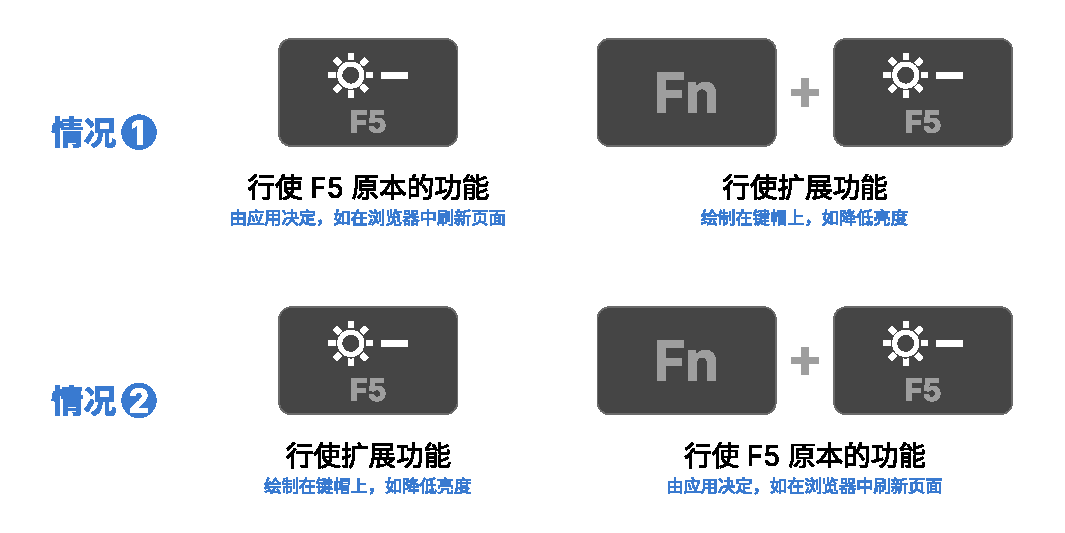
\includegraphics[width=.8\textwidth]{assets/basic/Fn_functions.pdf}
  \caption{\keys{F1} -- \keys{F12} 的两种功能情况}
  \label{fig:Fn_functions}
\end{figure}

你可以随便打开一个应用(比如浏览器),然后按 \keys{Alt + F4}。如果刚打开的应用退出了,就说明你的电脑属于上面两种情况中的第一种。如果没有反应,就属于第二种。

有些键盘提供了快捷的方法在这两种模式中切换。比如某些笔记本电脑键盘,可以通过按 \keys{Fn + Esc} 来切换这两种模式。另一些键盘可能需要使用专门的软件来进行调整,具体还请参考你的笔记本电脑或者键盘的说明书。

\begin{note}
	这意味着,对于那些包含 \keys{F1} -- \keys{F12} 功能键的快捷键,如果你按下后电脑没有反应,不妨在按住 \keys{Fn} 的同时再试一次——你的键盘有可能是上面的情况 2,\keys{F1} -- \keys{F12} 功能键只有在按住 \keys{Fn} 时才发挥原本的作用。
\end{note}

\section{「重启」不是关机再开机}

对今天大多数的电脑来说,「重启」过程并不等价于「先关机再开机」的过程。若在我们在文中提及了「重启」操作,请务必选择开始菜单中的「重启」选项重启电脑,而非将电脑关机后再手动打开。

\section{存储容量的单位}

我们对本书中使用的容量单位「TB」「GB」「MB」「KB」的关系约定如下:
\[
  1\,\mathrm{TB}=1024\,\mathrm{GB}=1024\times1024\,\mathrm{MB}=1024^3\,\mathrm{KB}=1024^4\,\text{字节}
\]
我们有时会略去这些单位最后的字母「B」,即文中可能用「1 T」来表示「1 TB」。

\begin{note}
  如果你有买过 U 盘,你会发现标称「128 GB」的 U 盘实际可用的容量只有 119 GB 左右。这是因为生产 U 盘的厂家用「1000 进位」来计算容量,而我们使用的 Windows 操作系统则用「1024 进位」来计算容量。为了避免换算带来的麻烦,本书与操作系统的用法保持一致,使用「1024 进位」。
\end{note}

\section{「设置」和「控制面板」}

在今天的大多数电脑上,「设置」app 用于对系统绝大多数的选项进行调整。我们可以在开始菜单中找到一个齿轮图标的应用,点击它就可以打开「设置」。按键盘上的 \keys{\Windows + I} 也可以打开它。文中,「打开系统设置」的说法均是指打开这个应用。

\begin{figure}[htb!]
  \centering
  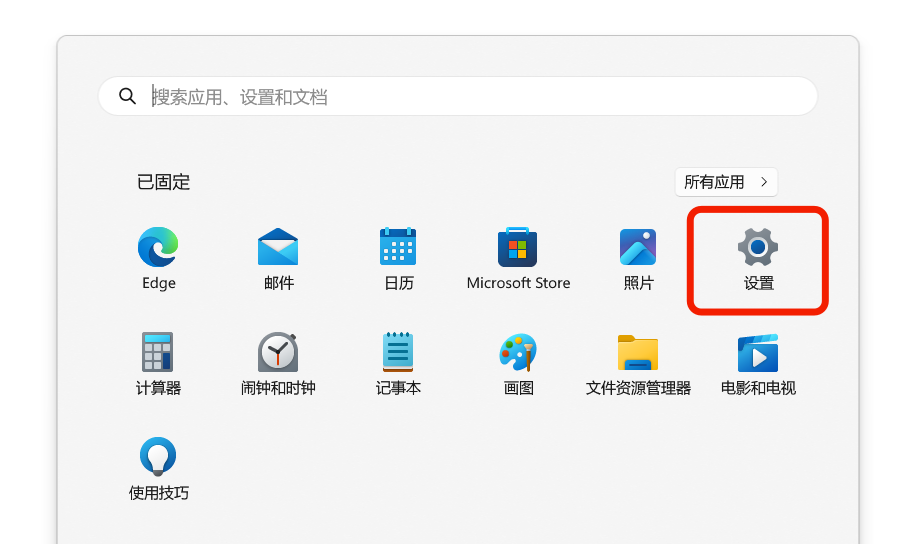
\includegraphics[width=.6\textwidth]{assets/basic/Settings.png}
  \caption{设置}
  \label{fig:Settings}
\end{figure}

你可能听说过「控制面板」这个词,它是 Windows 10 之前的 Windows 系统中用来调整系统设置的应用。在今天我们常用的 Windows 10 和 Windows 11 中,控制面板仍然存在,但它的功能已经被「设置」app 取代。只有当我们在文中明确使用「控制面板」一词时,才需要你使用它。

\practice

\begin{enumerate}
  \item 计算 1 GB 等于多少 KB?等于多少字节?假设一个汉字占两个字节,1 GB 大约可以记录多少个汉字?
  \item 尝试计算,一个按 1000 进位计算得到容量为 64 GB 的 U 盘,按 1024 进位计算得到的容量是多少?
  \item 在自己电脑上尝试这些快捷键:
    \begin{enumerate}
      \item \keys{\Windows + Shift + S} (仅限 Windows 10 / 11)
      \item \keys{Ctrl + Shift + Esc}
      \item \keys{\Windows + D}
    \end{enumerate}
  \item 如果你在用笔记本电脑,了解并体验它 \keys{F1} -- \keys{F12} 功能键的扩展功能。
\end{enumerate}
\chapter{认识你的电脑}
\label{cha:computer-and-its-components}

\begin{intro}
  或许电脑对你来说,是一个熟悉却又神秘的「黑箱」:它早已融入我们的生活,但我们却很少真正了解它的组成与结构。阅读完本章,你将找到这些问题的答案:

  \begin{itemize}
    \item 什么是「CPU」?别人说的「i5」「i7」都是什么?「双核」「四核」又是什么?
    \item 为什么说「内存」和「硬盘」不一样?存储东西的到底是内存还是硬盘?电脑特别卡,到底是内存不够还是硬盘不够?
    \item 我想玩游戏,选购电脑时应该关注什么方面?「显卡」是什么东西?
    \item 什么是「Windows」?那「Windows 11」又是什么?为什么苹果笔记本的系统界面看起来和我不一样?我用的是什么系统?
  在这一部分,我们将对「电脑」这种神奇的黑箱做一个简要的、整体的介绍。看完这一部分,你将可以找到这些问题的答案:
  \end{itemize}
\end{intro}

如今,电脑几乎「无所不能」,已经成为了我们生活和工作中不可或缺的一部分。每一台电脑内部,都充满了复杂的电子电路和元器件,它们是人类智慧的结晶,构成了电脑的「硬件」部分。而在这冷冰冰的硬件之上,「软件」赋予了电脑生命与功能——从办公、学习到娱乐,各种软件让我们的生活更加便捷。可以说,硬件如同电脑的「身体」,软件则是电脑的「思维」,它们共同构成了「电脑」这个有机体。

本章将引领你深入认识自己的电脑:从最基础的硬件开始,我们将逐一介绍它们的功能与作用,并分析这些硬件如何影响电脑的性能。接着,我们将了解运行在这些硬件之上的各种软件,介绍它们与硬件的协同和配合,让你对电脑的构成和运行有一个更加全面的了解。

\section{电脑内部的硬件} 

本节我们将介绍电脑内部的那些关键硬件。即使你并没有亲眼见过各种硬件模块的模样,但通过这一节的介绍,你也会对它们形成基本的了解。

在开始之前,我们先假设这样一个场景:某位老师收集了一个班的作业,现在需要批改它们,如下图所示。

\begin{figure}[htb!]
  \centering
  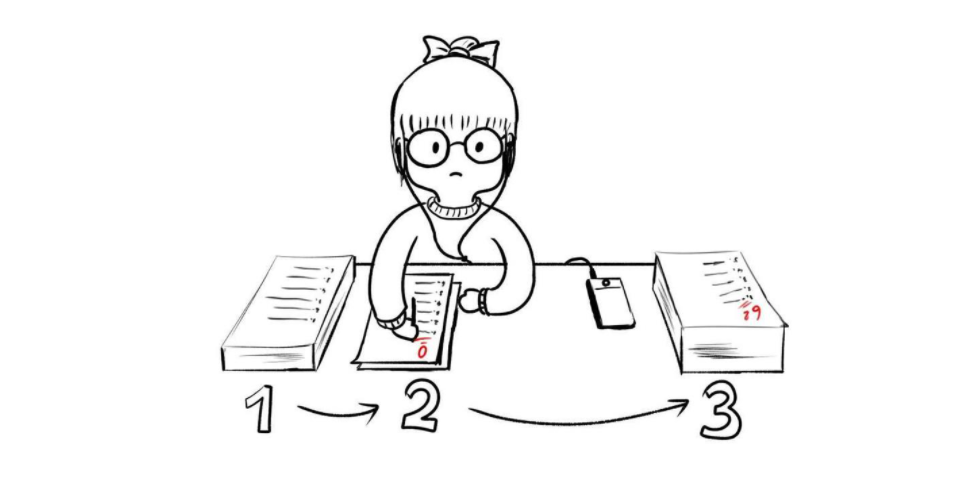
\includegraphics[width=.5\textwidth]{assets/basic/Teacher_and_homework.png}
  \caption{正在批改作业的老师}
  \label{fig:teacher-and-homework}
\end{figure}

我们可以把老师批改作业的过程分解成下面的步骤:

\begin{enumerate}
  \item 老师将这一摞作业堆在办公桌的一边,腾出办公桌的中央和另一边。
  \item 现在,老师取下这一摞作业中的一小叠,放在办公桌中央,开始伏案批改。
  \item 老师批改完了这一小叠作业,然后将它们放在办公桌的另一边,摞成新的一沓。
  \item 重复步骤 2 和步骤 3,最终老师完成了全部作业的批改,这时批改完的作业全部在办公桌的另一边。
\end{enumerate}

这个例子有什么用呢?请先记住它,它将帮助我们更好地理解电脑硬件的工作原理。

\subsection{处理器(CPU)}

中央处理器(Central Processing Unit),简称「处理器」,英文简写「CPU」,是电脑内部最重要的一枚芯片,可以想象成是电脑的「大脑」。在上面的例子中,老师就相当于电脑中的处理器:老师的作用是批改作业,从而完成教学任务;处理器的作用是进行各种运算,从而实现电脑不同的功能。

你一定注意到过,电脑会发热——热到需要用一个风扇给它降温,这热量中有很大一部分就是处理器发出来的。如果你有关注过时事和新闻,中美贸易战之中关键的一环,正是处理器芯片。下图中,左边是一枚台式机的 CPU,右边是一枚笔记本电脑的 CPU。

\begin{figure}[htb!]
  \centering
  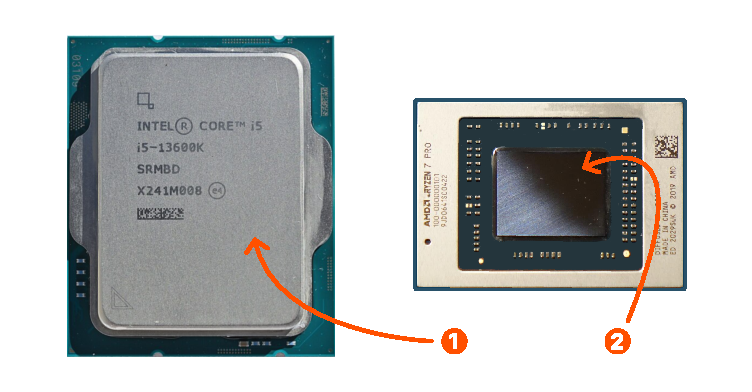
\includegraphics[width=.6\textwidth]{assets/basic/Two_CPUs.pdf}
  \caption{常见的台式机和笔记本电脑的处理器芯片}
  \label{fig:Two_CPUs}
\end{figure}

\begin{note}
  你可能会疑惑:这两个 CPU 为什么看起来很不一样?这是因为笔记本 CPU 为了节省空间,会直接将 \underline{➋「晶片」}(芯片的核心部分,由硅制成)裸露在外;而台式机 CPU 为了保护晶片,会在其外罩上一层 \underline{➊ 金属盖}。
\end{note}

处理器是电脑工作的核心,因此,\regcolor{处理器的性能就很大程度上决定了电脑的性能,决定了我们使用这台电脑流不流畅、玩游戏卡不卡、工作效率高不高}。在今天,全世界电脑芯片基本上是由两家美国公司设计\footnote{事实上,芯片的「设计」和「制造」两件事是不一样的,就像能设计出房屋的建筑师不一定会到工地上去砌墙。英特尔能够自行完成从设计到制造整条生产链,而 AMD 只能完成设计,它的处理器是由专门负责制造芯片的厂商(例如台积电)生产的。}的,其中一家叫做「英特尔」(Intel),另一家叫做「AMD」。

\begin{itemize}
  \item 英特尔公司现在主要的 CPU 产品线称作「酷睿」(Core),而「酷睿」系列又分成了三个子系列,每个子系列都有不同档次的产品。
    \begin{table}[htb!]
      \centering
      \caption{英特尔CPU产品系列}
      \label{tab:Intel-CPUs}
      \begin{tblr}{
        colspec = XX[2]X[4]X[4],
        cells = {c, m},
        cell{Z}{2-Z} = {j},
        row{1} = {fg = white, bg = missing, font = \bfseries},
        row{even} = {MissingLightBlue},
      }
        \toprule
        & 传统酷睿系列 & 酷睿 Ultra 系列 & 酷睿数字系列 \\
        \midrule
        低端 & 酷睿 i3 & 酷睿 Ultra 3 & 酷睿 3 \\
        中端 & 酷睿 i5 & 酷睿 Ultra 5 & 酷睿 5 \\
        高端 & 酷睿 i7 & 酷睿 Ultra 7 & 酷睿 7 \\
        顶尖 & 酷睿 i9 & 酷睿 Ultra 9 &  ---\footnotemark \\
        说明 & 传统的酷睿系列,自 2008 年起沿用至今 & 2023 年发布的新系列,主要应用在高端笔记本电脑产品上,增加了针对 AI 应用的优化 & 2024 年发布的新系列,针对笔记本电脑产品进行了能耗方面的优化 \\
        \bottomrule
      \end{tblr}
    \end{table}
    \footnotetext{截至 2024 年 12 月,英特尔并没有推出酷睿 9 系列的 CPU。}\\
    大多数使用英特尔 CPU 的电脑,机器表面会贴一个类似左下图的蓝色(或灰色、黑色)贴纸。对于笔记本电脑,通常贴在键盘下方或机器背面;而对于品牌台式机,则通常贴在机器正面、侧面或顶面,如右下图所示。
    \begin{figure}[htb!]
      \centering
      
\includegraphics[width=.7\textwidth]{assets/basic/Intel_sticker.png}
      \caption{英特尔的贴纸}
      \label{fig:Intel_sticker}
    \end{figure}\\
    \begin{figure}[htb!]
      \centering
      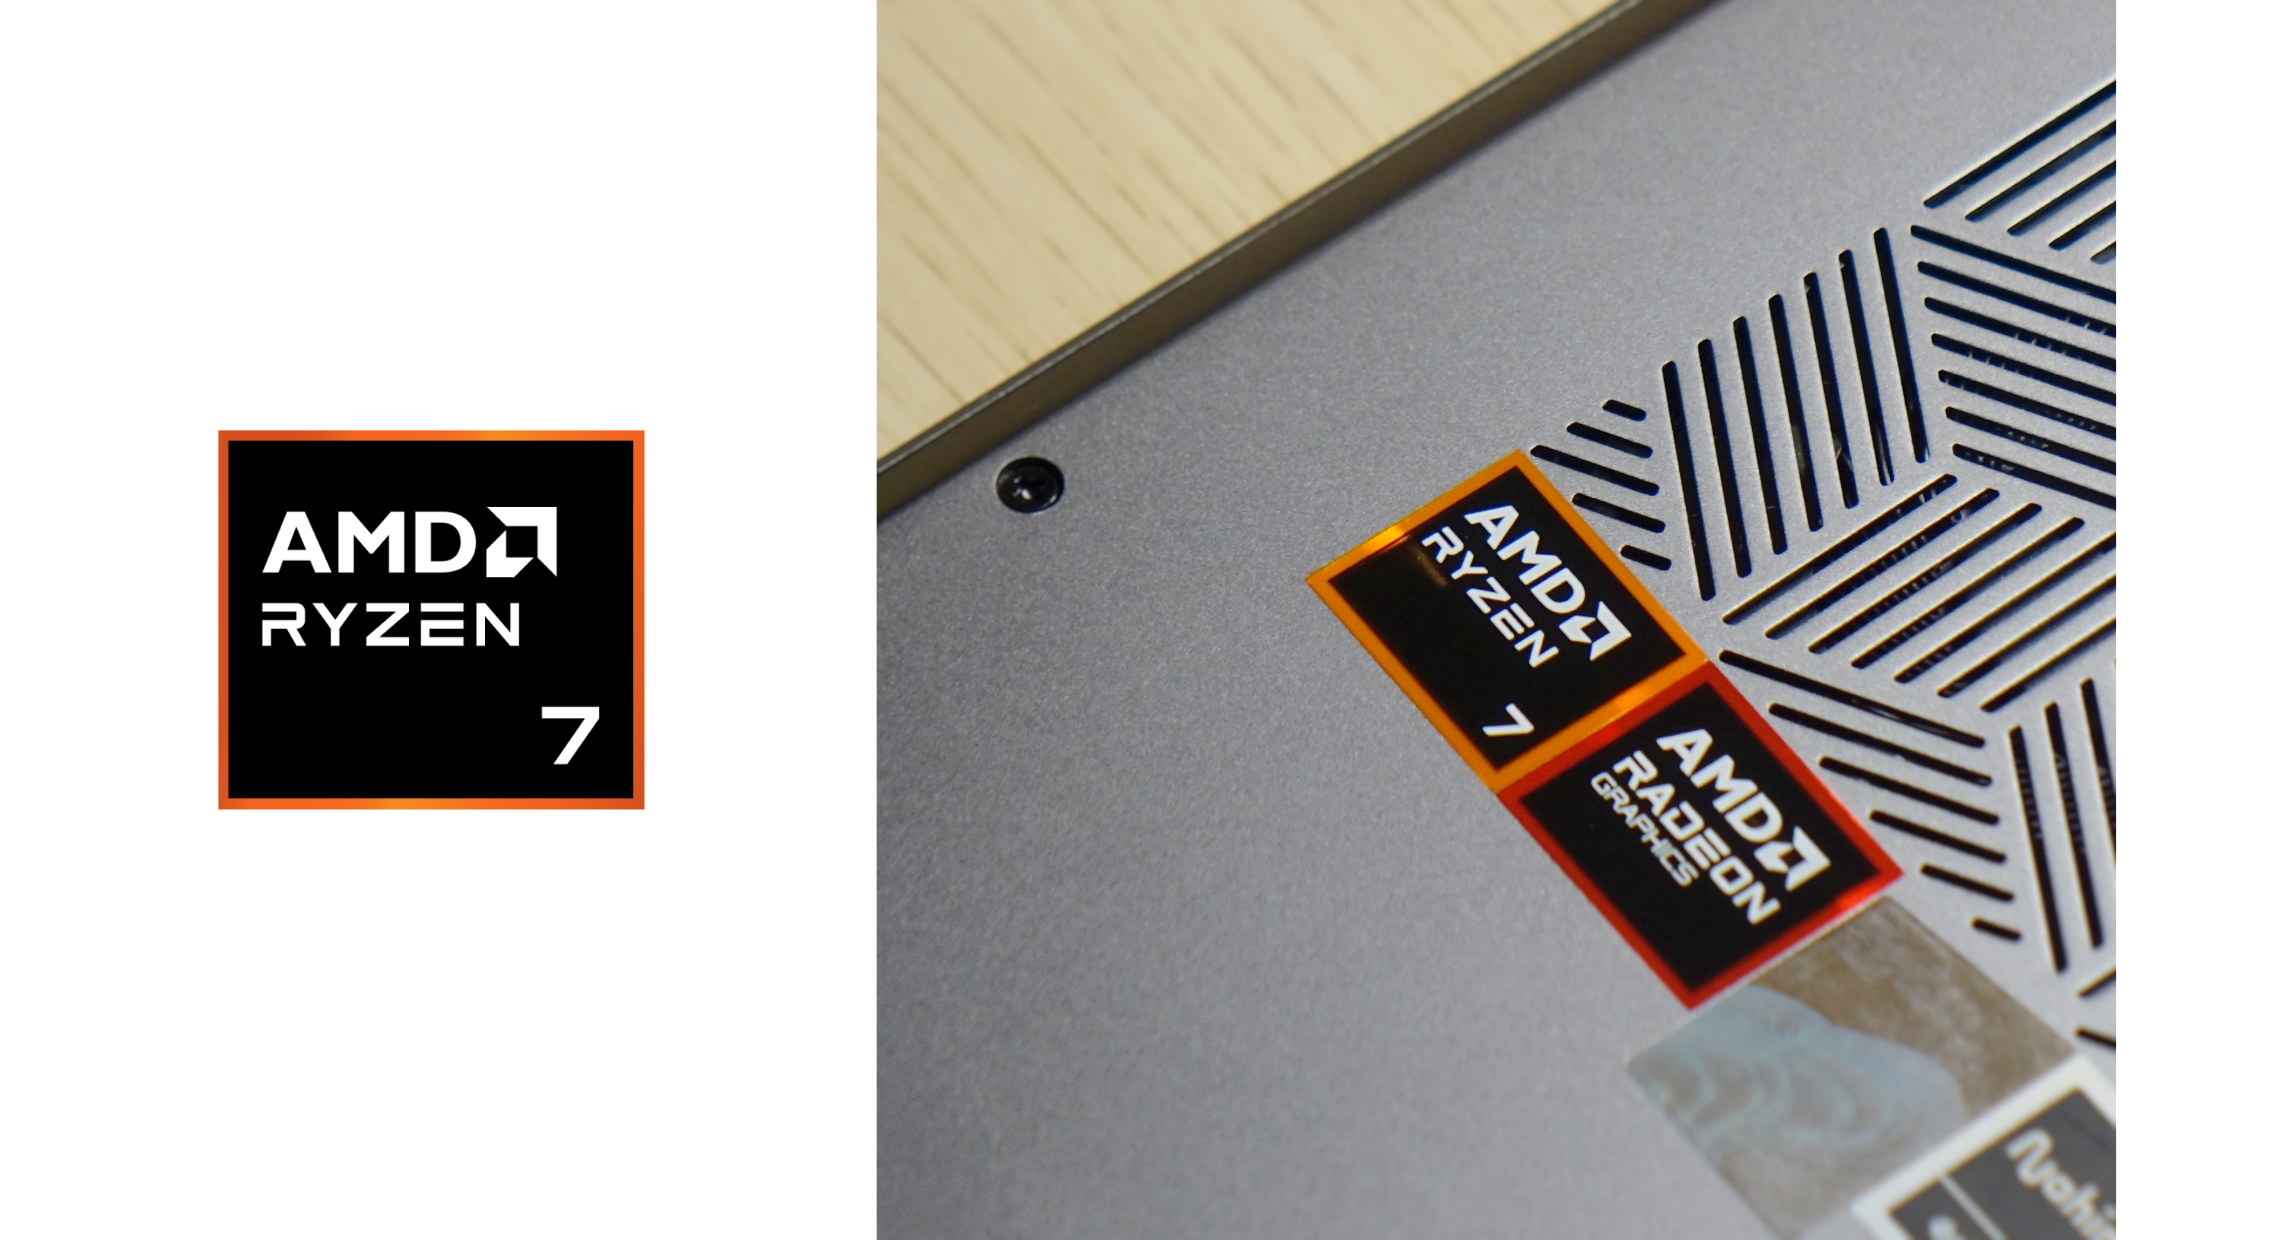
\includegraphics[width=.6\textwidth]{assets/basic/AMD_sticker.png}
      \caption{AMD的贴纸}
      \label{fig:AMD_sticker}
    \end{figure}
  \item AMD 公司现在主要的 CPU 产品线称作「锐龙」(Ryzen),而锐龙系列也分成了 3 个档次——「R5」「R7」和「R9」\footnote{其实还有 R3,但是很少在消费市场见到。}。大多数使用 AMD CPU 的电脑会粘贴类似图 \ref{fig:AMD_sticker} 的橙黑或橙灰色贴纸。
\end{itemize}

\begin{note}
  除了英特尔和 AMD 之外,亦有一些厂商能够生产电脑的 CPU,例如苹果、高通,以及国产厂商龙芯、华为等。不过,这些厂商生产的 CPU 与英特尔、AMD 的 CPU 往往并不兼容,使用这些 CPU 的电脑需要使用专用的系统和软件。想了解更多有关这些 CPU 的细节?请阅读本书超越篇的\nameref{cha:program-and-arch}。
\end{note}

我们常常说一台电脑是「双核」「四核」的,这里的「双核」「四核」就是处理器中的概念。今天,几乎所有 CPU 都在芯片中安装了多个「核心」,相当于一个个协同起来的独立的小处理器。例如,「双核」意味着在一枚处理器芯片上集成了两个核心,相当于两个大脑协同工作,当我们需要用电脑同时做很多事情的时候就有所裨益。同理,「四核」「八核」就是在一个芯片上集成了四个甚至是八个核心。现在,一些 CPU 还使用「大小核」设计,混合使用大小两种规格不同的核心,来实现性能和功耗之间的平衡。下图中,左方是一枚四核 CPU 示意图,右方则是一枚采用大小核设计的六核处理器示意图(图片非实际比例)。

\begin{figure}[htb!]
  \centering
  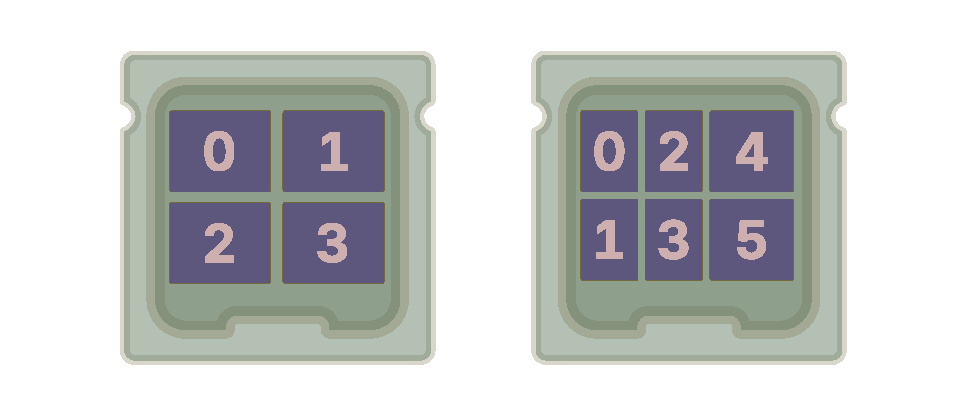
\includegraphics[width=.6\textwidth]{assets/basic/Multicore.pdf}
  \caption{多核CPU示意}
  \label{fig:Multicore}
\end{figure}

然而,核心数只能反映「脑子多不多」,但无法刻画「一个脑子有多快」。要衡量一颗 CPU 的性能,除了直观地根据厂商划定的这些低中高端系列之外,「主频」也是一个重要的参考。所谓「主频」指的是这 CPU 一秒种能够「工作」的次数,人们通常使用单位「GHz」来标注它。1 GHz 就表示「1 秒能『工作』10 亿次」。CPU 通常有一个「基准频率」和「加速频率」,前者是 CPU 正常工作时的稳定频率,后者则是在短时间内应对复杂任务时能达到的最高频率。目前,常见的台式机 CPU 的基准频率和加速频率能达到 3 GHz 和 5 GHz,而笔记本则在 2 GHz 和 4 GHz 左右。

需要强调的是,\regcolor{并不是说核心数越多、主频越高的处理器性能一定越好},更\regcolor{不是说 i7 处理器就一定比 i5 更好},也\regcolor{不是说英特尔和 AMD 有孰优孰劣之分}。我们应该综合理解这些概念:每个品牌都会随着时间推移一代代地更新,每一代都有着的不同系列,有的系列高端,有的系列低端;每个系列也都有自己的不同型号,有的型号性能强,有的型号性能弱。CPU 的性能并不与某一个因素呈线性的关系,而是多个因素叠加的结果。

按 \keys{Ctrl + Shift + Esc} 打开「任务管理器」,选择【性能】页面,就能看见 CPU 的型号、基准频率(标注为【基准速度】)和核心数(标注为【内核】)。

\begin{note}
  你也可以右击【开始按钮】,选择【任务管理器】来打开「任务管理器」。
\end{note}

\begin{figure}[htb!]
  \centering
  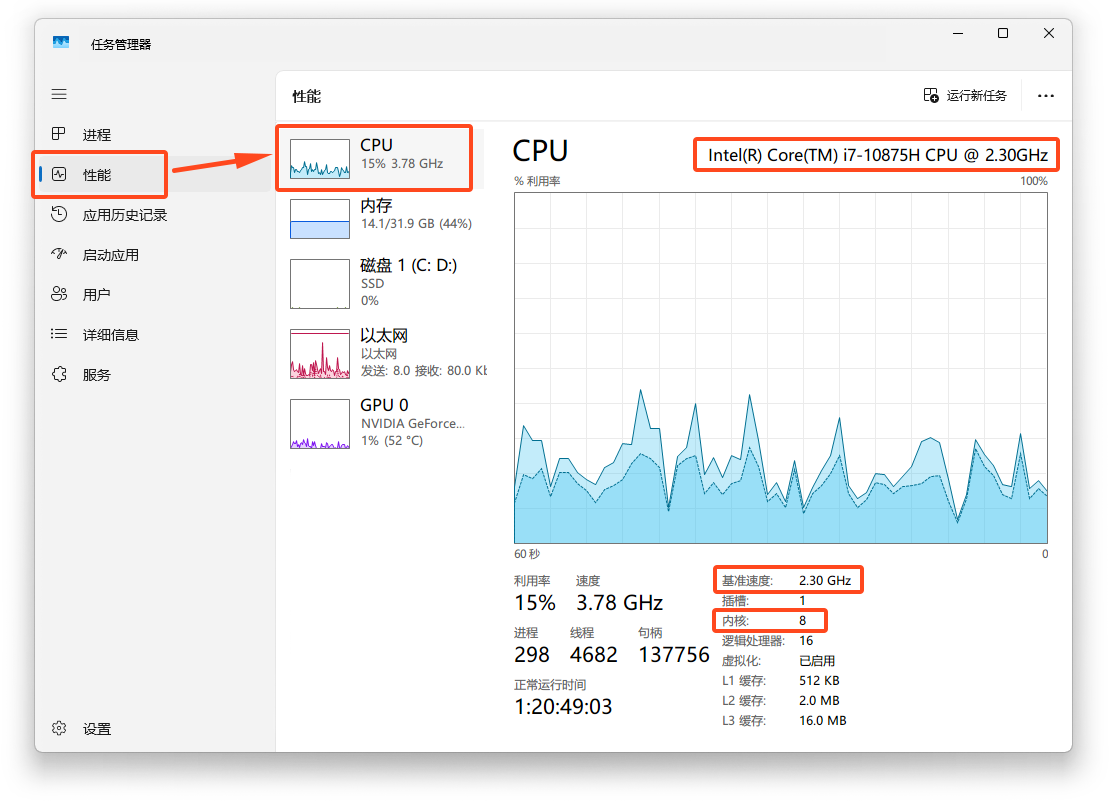
\includegraphics[width=.65\textwidth]{assets/basic/Check_CPU.png}
  \caption{在任务管理器看看CPU}
  \label{fig:Check_CPU}
\end{figure}

\subsection{内存(RAM)}

紧接着,我们介绍能直接与处理器交流的部件——内存,英文简写「RAM」。上一小节提到,处理器相当于大脑,但与大脑不同的是,处理器只能\regcolor{处理}数据,而这些待处理的数据,需要依赖外部的元件来临时存放。内存就是用来临时存放数据的。

内存的核心组件是一个个黑色的「内存芯片」。目前,内存芯片的主要生产厂商集中在韩国和中国台湾。这些芯片通常被排列在条形电路板上,形成一个模块,方便插入电脑主板进行更换或升级。这样的整体被称为「内存条」。如下图所示,左侧展示的是台式电脑使用的内存条,而右侧则是笔记本电脑使用的版本。不过,\regcolor{为了节省内部空间,很多笔记本电脑选择将内存芯片直接焊接在主板上,这种设计的内存无法更换或升级}。

\begin{figure}[htb!]
  \centering
  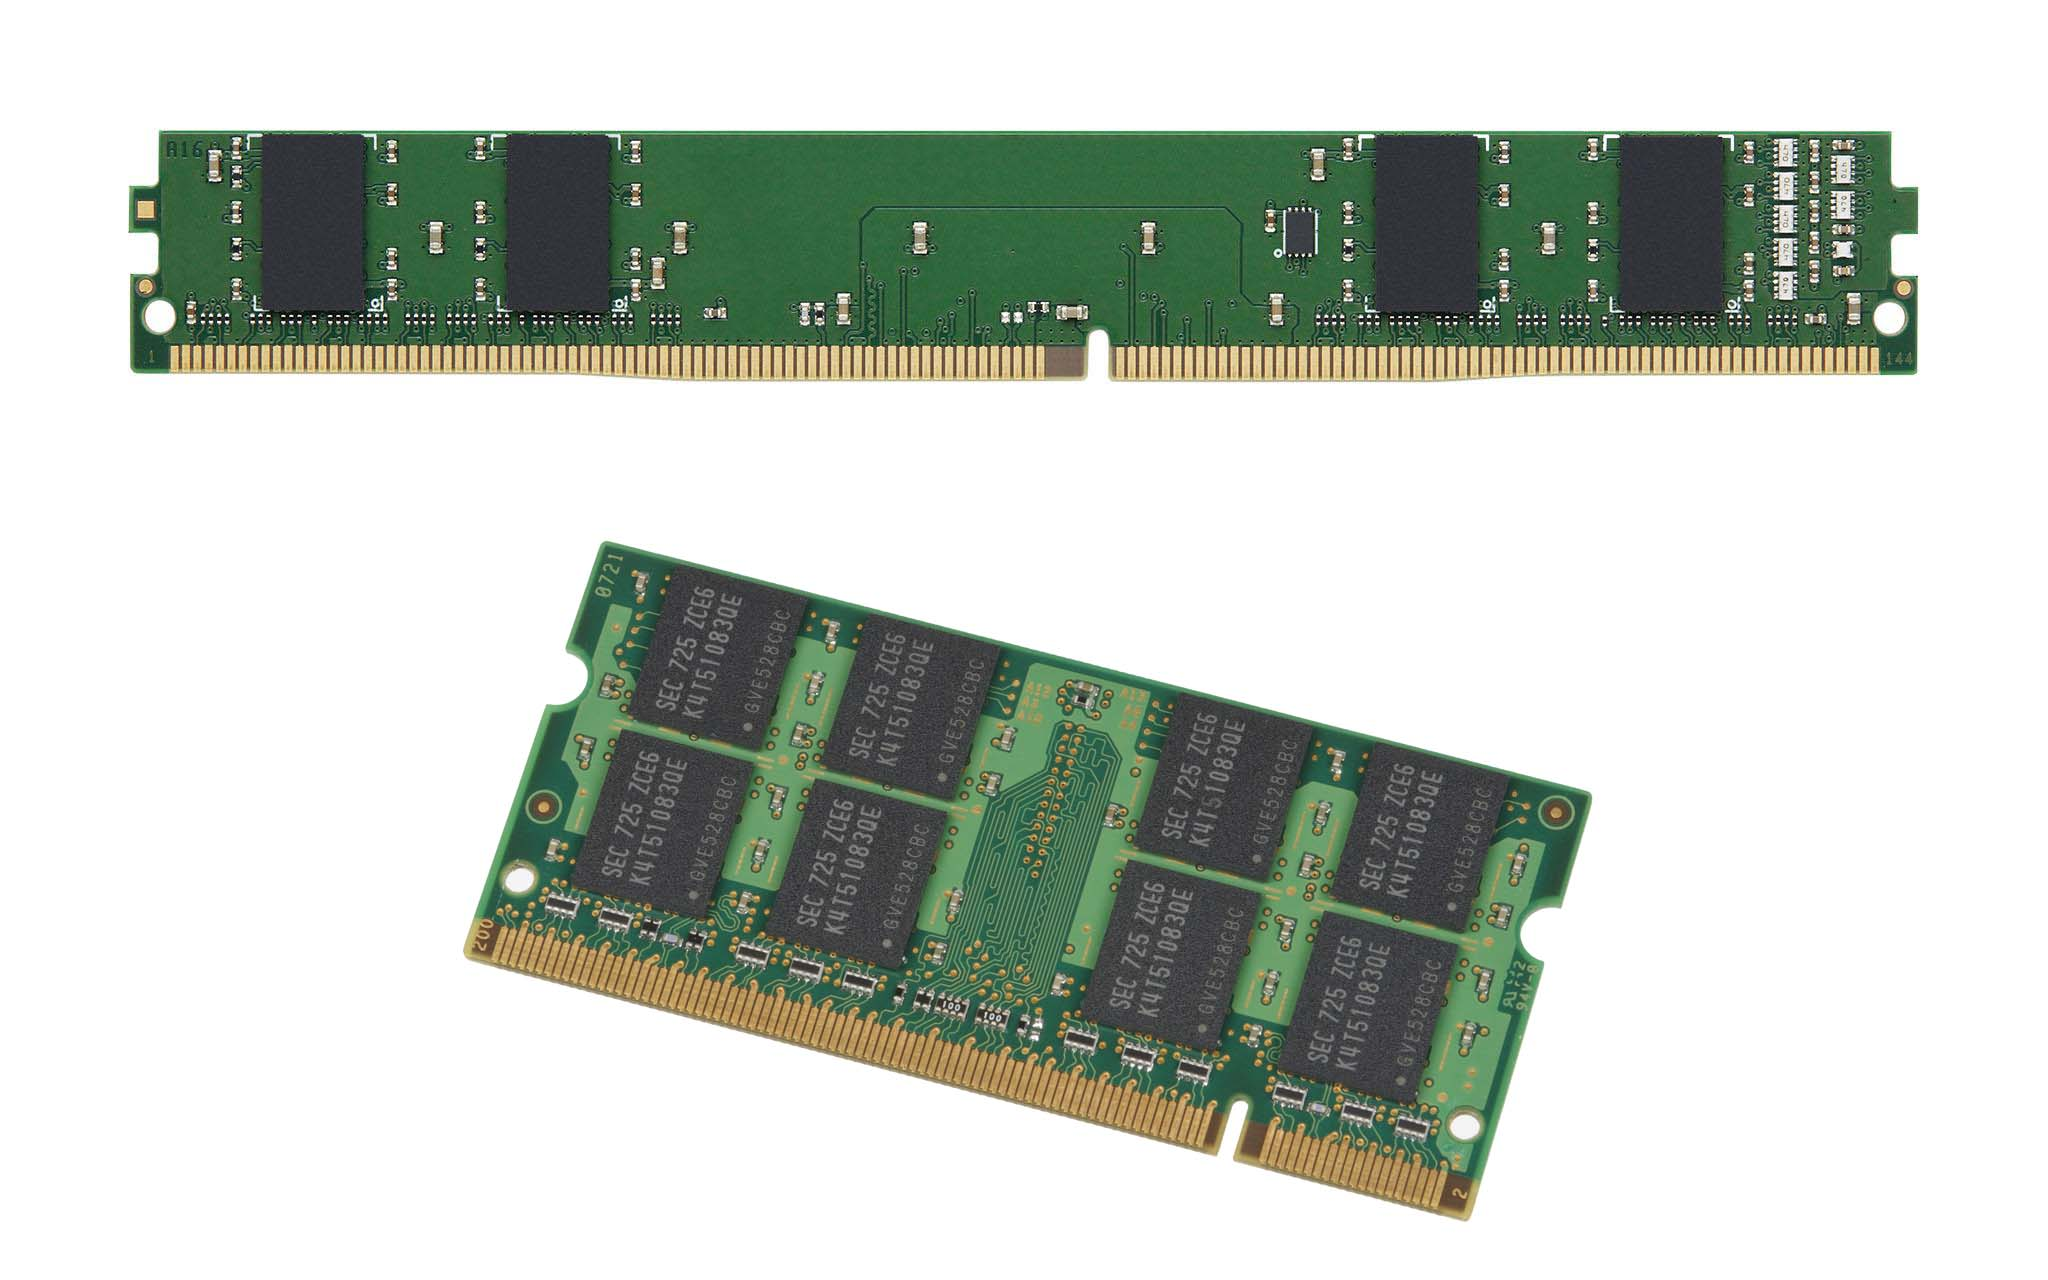
\includegraphics[width=.7\textwidth]{assets/basic/RAMs.jpg}
  \caption{不同的内存条}
  \label{fig:RAMs}
\end{figure}

前文说,内存直接与处理器进行数据交流。与处理器那极快的运算速度相匹配,内存的读取与写入速度也是极快的。但内存有一个特点——\regcolor{断电即丢失数据}。也就是说,当你电脑关机,内存中的数据便不复存在,又回到白纸一块。这种特性决定着,内存只能用来在电脑工作时临时存储信息。

回到前面老师批改作业的场景。办公桌的中央区域可以理解为「内存」:老师将作业放在办公桌中央批改,是因为这里改起来最方便;处理器将数据放在内存中处理,是因为这里读取和写入速度最快。办公桌中央不能总是放着东西,不然会弄乱、弄丢;内存中的数据一旦断电就会消失,因此总是临时的。

在 21 世纪初,电脑内存的容量不大,有 512 MB 已经不得了了。但随着科技发展,现如今,大容量内存已经司空见惯。在今天,要想让一台电脑能基本流畅运行,内存容量应当至少有 8 GB。当然这东西倒是多多益善,就像更大的桌子能摆更多东西一样,\regcolor{更多的内存意味着更多的空间来让处理器存放数据,也就意味着电脑能同时处理更多的任务,基本意味着电脑更加流畅。}据我们的经验,在目前(2024 年),16 GB 的内存对于日常使用已经够用;但如果你有大型游戏、三维建模、大型软件开发等需求,选择 32 GB 乃至更大的内存会更加合适。

\begin{note}
  对应到手机中,内存有时会被手机厂商称为「运行内存」,不过我们不推荐如此称呼。原因请参见下面「硬盘」一节。
\end{note}

在任务管理器的【性能】页的【内存】一栏,你可以看见自己电脑的内存总量等信息。

\subsection{硬盘}

内存是用来临时存储数据的,而硬盘则是用来长久保存数据的。与内存相比,硬盘的读写速度要慢得多,但存在硬盘中的数据不会因为断电而轻易消失,因此,硬盘是数据的最初的起点和最终的归宿:处理器在一开始,从硬盘中取出数据放入内存,在内存中处理数据,处理完成之后,再将新的数据放回硬盘。

\begin{note}
  所以,你电脑的所有资料都存在硬盘里。想直接拿走你的资料,应该去拿硬盘,而不是拿走显示器或别的什么东西。
\end{note}

\regcolor{除了各种各样的数据——各种文档、图片、音乐——之外,电脑上各种各样的软件本身,也是存放在硬盘里面的。}相信你在手机上有过这样的经验——手机的「存储空间」不够用,除了删掉一些不需要的照片、视频外,卸载不常用的 app 也是一个快捷的办法。在电脑上,情况是一样的:卸载软件,释放的其实就是硬盘上的空间。

\begin{figure}[htb!]
  \centering
  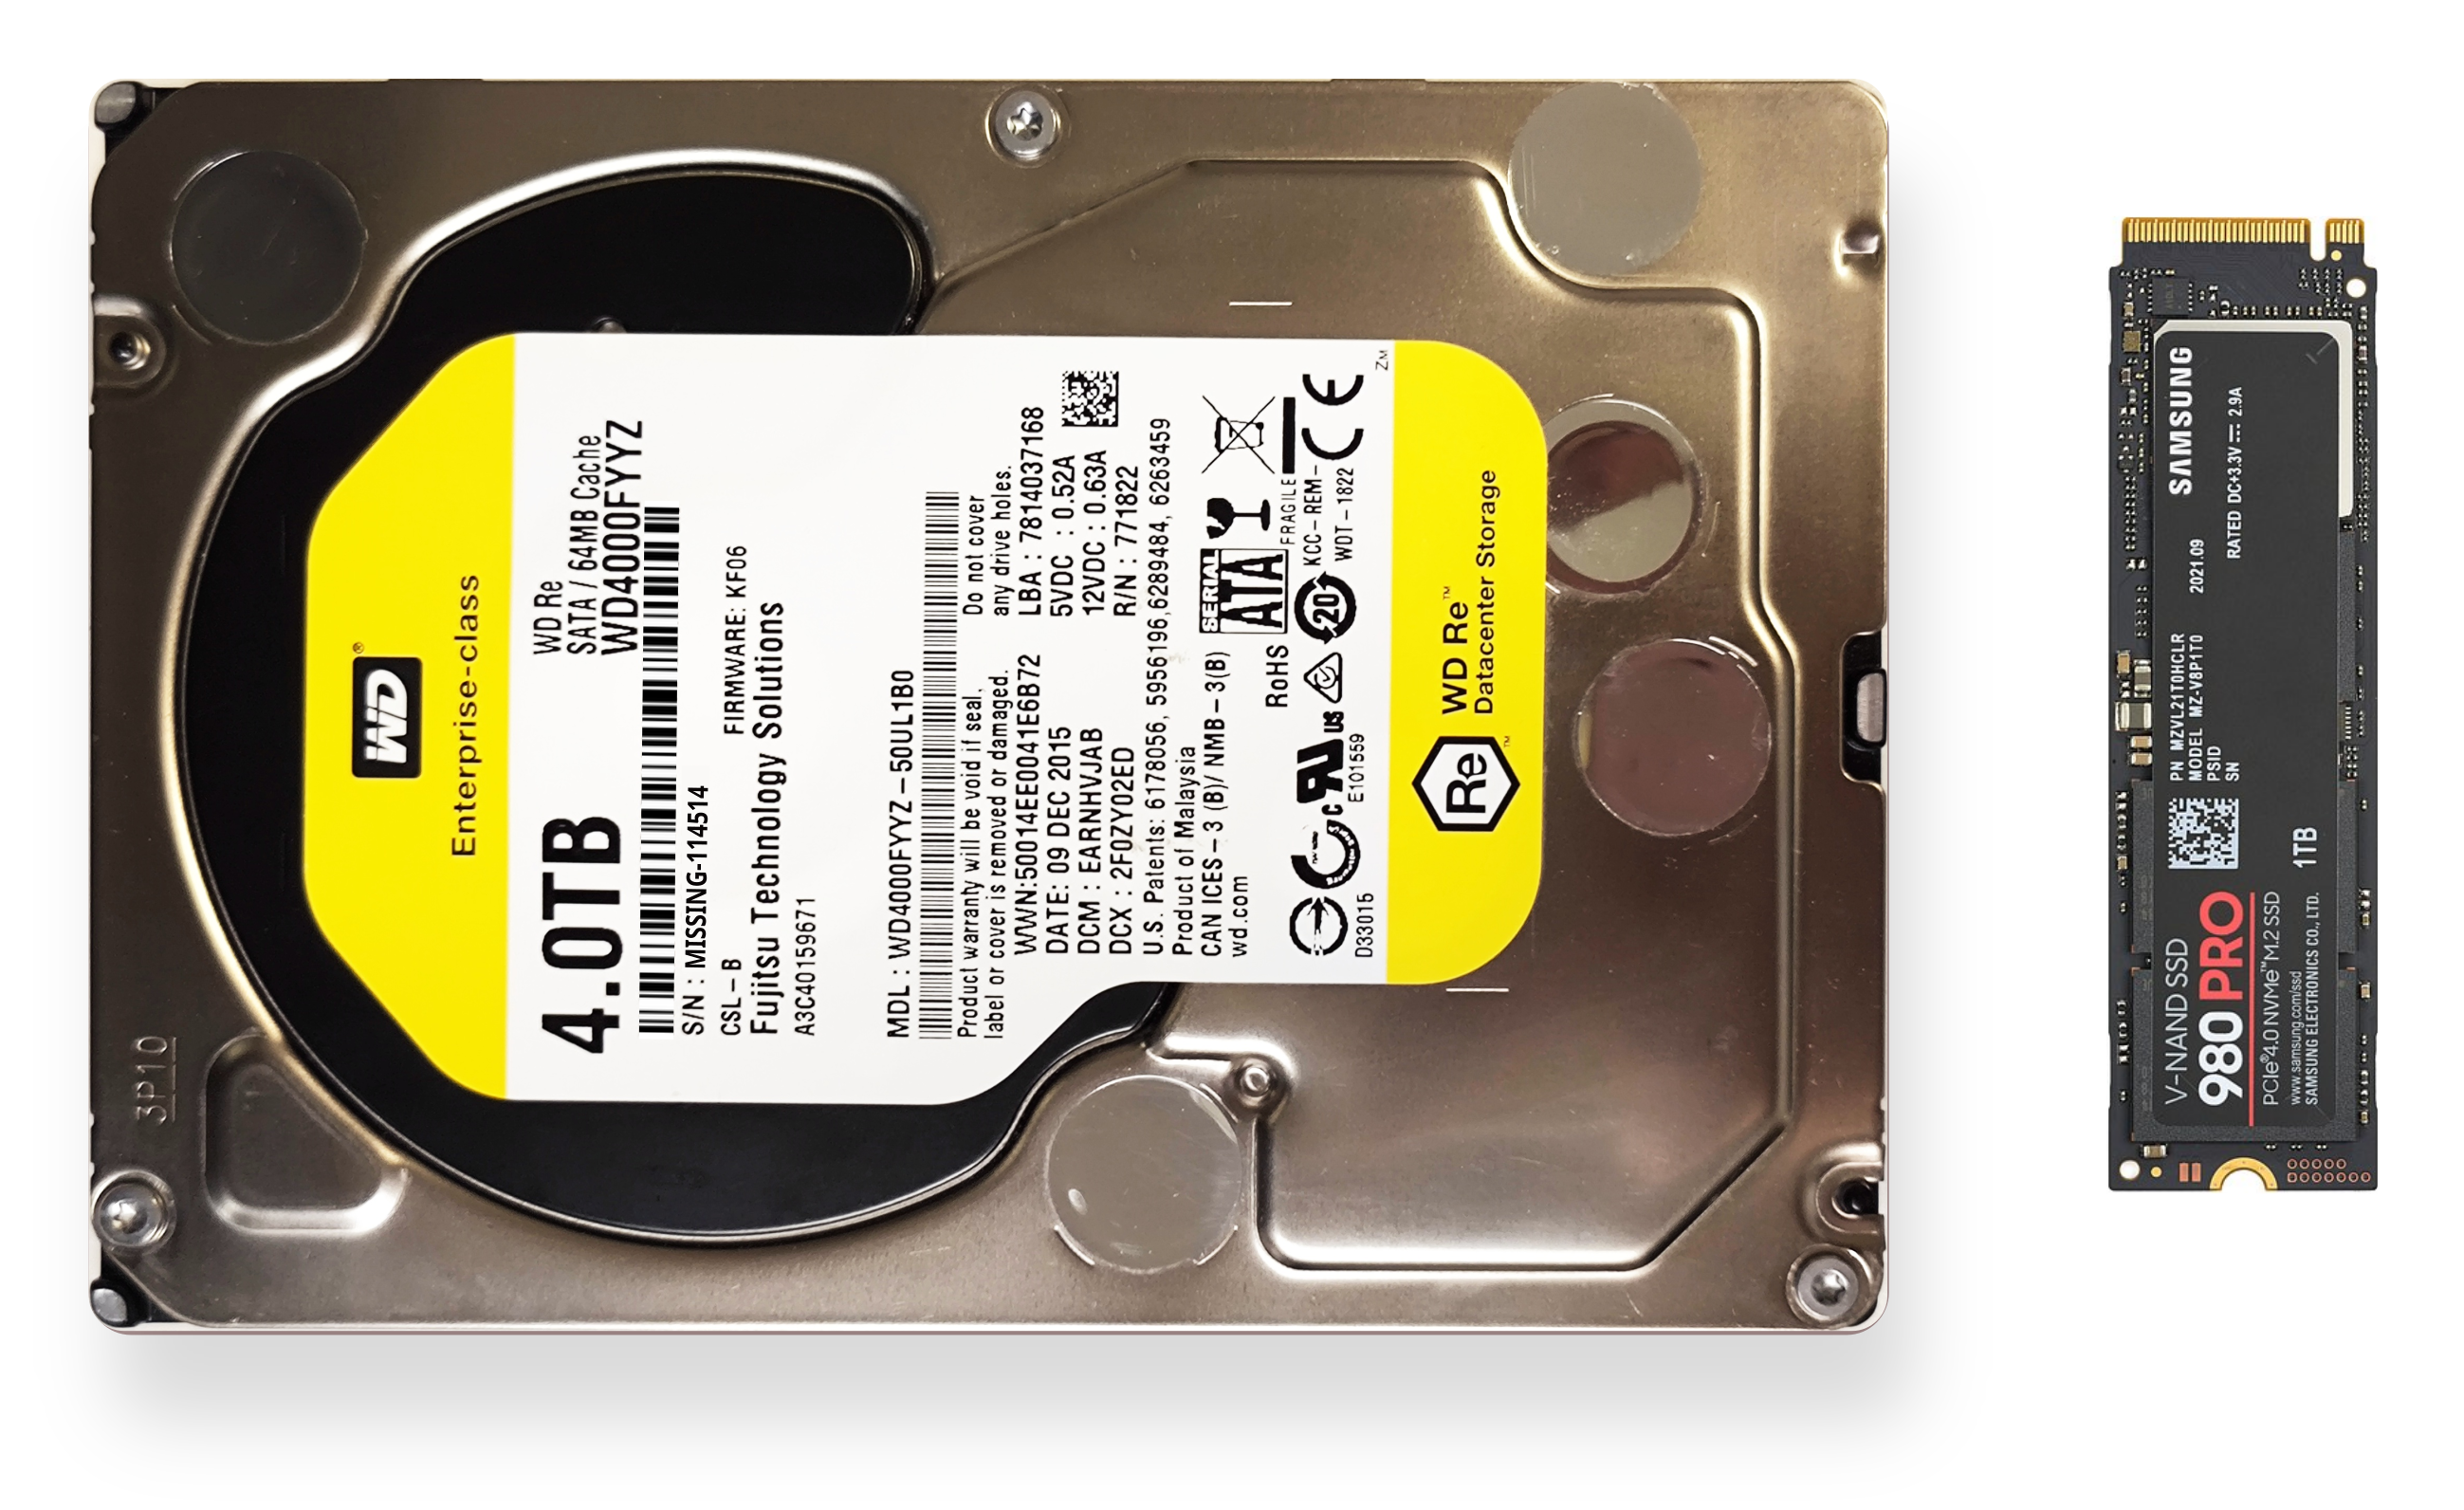
\includegraphics[width=.7\textwidth]{assets/basic/HDD_and_SSD.png}
  \caption{常见的硬盘}
  \label{fig:HDD_and_SSD}
\end{figure}

在前面老师批改作业的场景当中,办公桌两侧堆作业的地方可以理解为「硬盘」:大量的作业被堆在那里,整齐摆放,不会弄散、弄丢,但老师总是要把作业取到趁手的地方(办公桌中央)来批改;大量的数据被存在硬盘里,不会因为断电就丢失,但处理器总是要把数据放在快速的地方(内存)来处理。

简单来说,硬盘现在分为两种,一种叫「机械硬盘」(Hard Disk Drive,简称「HDD」),如图 \ref{fig:HDD_and_SSD} 左侧所示,容量大、价格低、速度更慢,利用电磁原理存储数据。另一种叫「固态硬盘」(Solid State Drive,简称「SSD」),如图 \ref{fig:HDD_and_SSD} 右侧所示,容量小、价格高、速度较快(但远远没有内存那么快)。SSD 用芯片存储数据,但这种芯片和内存的那种不同,断电还能保持数据。不过,不管是哪种硬盘,如果硬盘许久不用(不给它通电),那里面的数据也会慢慢消失,固态硬盘大约是 3 至 5 年,而机械硬盘最多 20 年——所以,对于存了东西但没有装入电脑的备用硬盘,要定期拿出来通电运转一下。

在今天(2024 年),标称容量 1 TB 的固态硬盘大约 500 元,机械硬盘大约 300 元;标称容量 2 TB 的固态硬盘大约 800 元,机械硬盘大约 400 元。因此,有些电脑会用一块小容量(512 GB 及以下)的固态硬盘,搭配一块大容量(1 TB 及以上)的机械硬盘来实现各自功能的互补。但也有一些中高端电脑会直接选用一整块大容量(比如 1 TB 甚至 2 TB)的固态硬盘而不再使用机械硬盘。

\regcolor{一块硬盘的空间可以被划分成不同的「盘」(学名叫「分区」)来更好地使用}。双击桌面上的【此电脑】来打开「文件资源管理器」,你看到的「C 盘」「D 盘」就是各个分区。在下一章\nameref{cha:file-and-file-management},我们将向你介绍如何管理好自己硬盘上的东西。 

\begin{figure}[htb!]
  \centering
  
\includegraphics[width=.8\textwidth]{assets/basic/Partitions.png}
  \caption{一些分区}
  \label{fig:partitions}
\end{figure}

\begin{note}
  如果你在桌面上没有看到【此电脑】图标,你也可以按下 \keys{\Windows + E} 组合键来打开文件资源管理器,然后在左侧的导航栏中找到【此电脑】。

  如果你想在桌面上显示【此电脑】图标,请先打开系统设置,然后选择【个性化】,找到【主题】。

  \begin{center}
    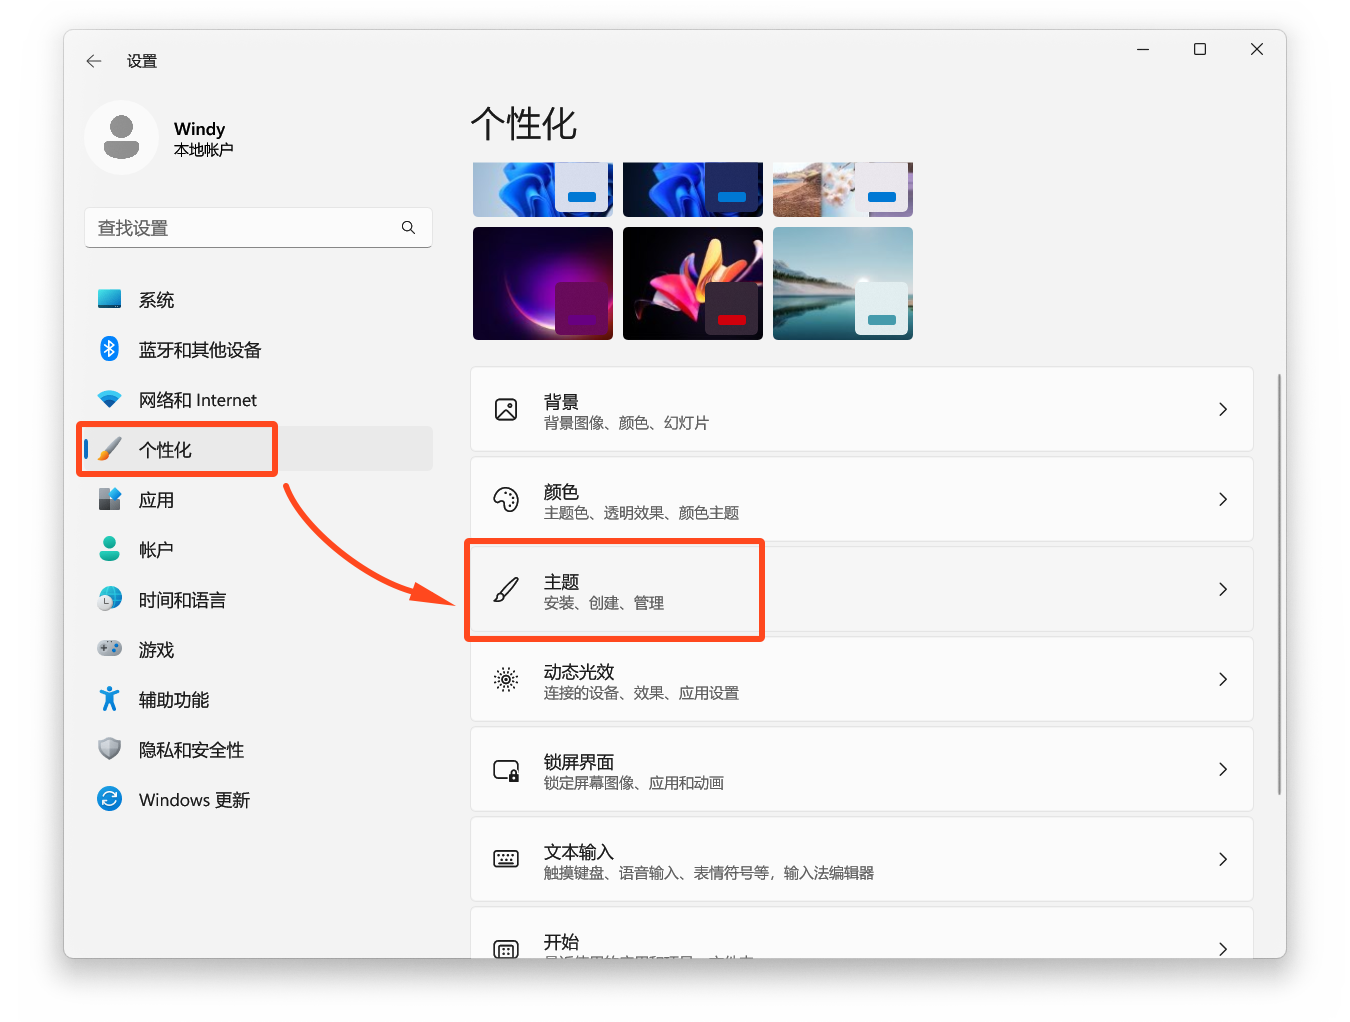
\includegraphics[width=.6\textwidth]{assets/basic/Open_personalization_in_settings.png}
    \captionof{figure}{找到【主题】设置}
    \label{fig:Open_personalization_in_settings}
  \end{center}

  然后,在界面下方找到【桌面图标设置】(Windows 10 可能显示在界面右方),勾选【计算机】(即【此电脑】),再点击【应用】。你也可以把其他几个常用的图标勾选上,比如【用户文件】、【回收站】等。

  \begin{center}
    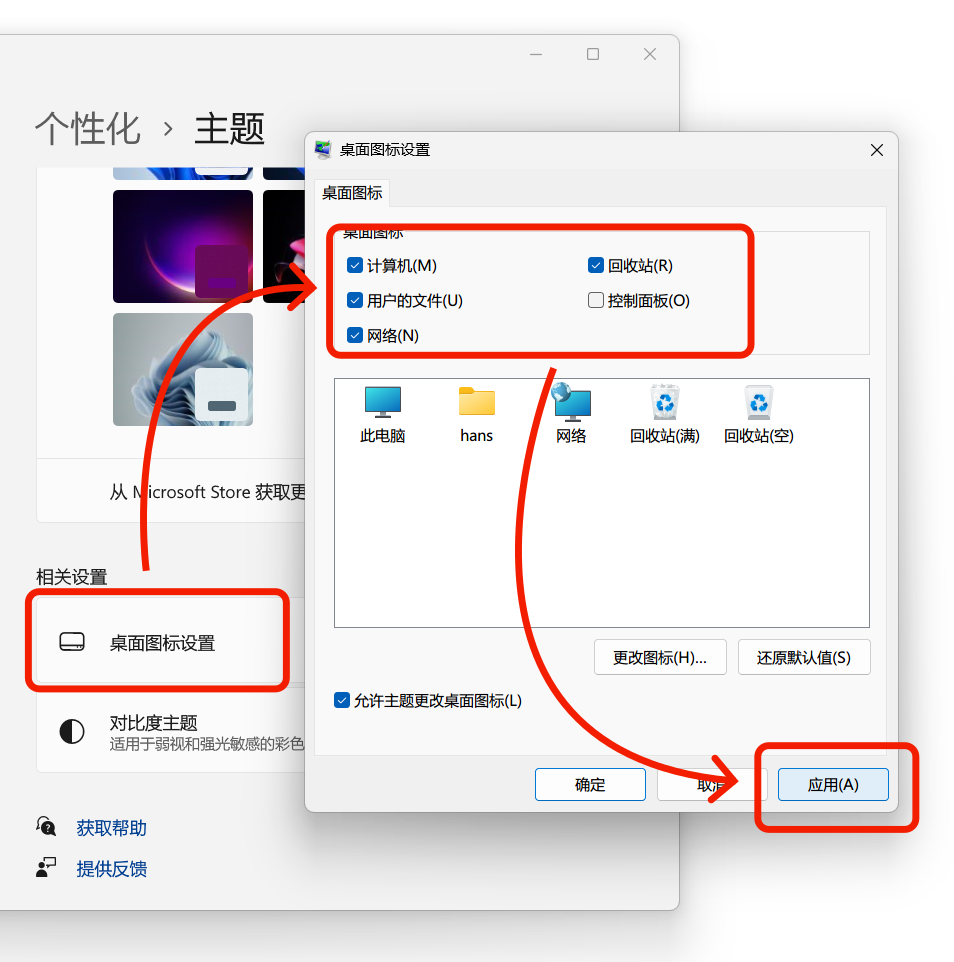
\includegraphics[width=.6\textwidth]{assets/basic/Select_This_PC.png}
    \captionof{figure}{选择要显示的图标}
    \label{fig:Select_This_PC}
  \end{center}

  这样,你的桌面上就会显示那些对应的图标了。
\end{note}

\regcolor{硬盘对电脑使用体验的影响,主要是打开软件的速度,包括开机的速度。}这是很容易理解的,因为数据和软件本身原先都是存在硬盘里的,处理器从硬盘里取数据的速度就直接影响着软件启动或者说加载的时间。

\begin{note}
  手机中用类似固态硬盘一样的芯片来存储数据,有些手机厂商和商家会称之为「内置存储」「存储内存」甚至是「内存」,但它\regcolor{完全不是}内存。这是为什么有人会弄混内存和硬盘的根源之一。人们常说的「手机内存不够」,指的往往是存储空间(可以称「手机的硬盘」)不够,而不是真正的「内存不够」。
\end{note}

\begin{figure}[htb!]
  \centering
  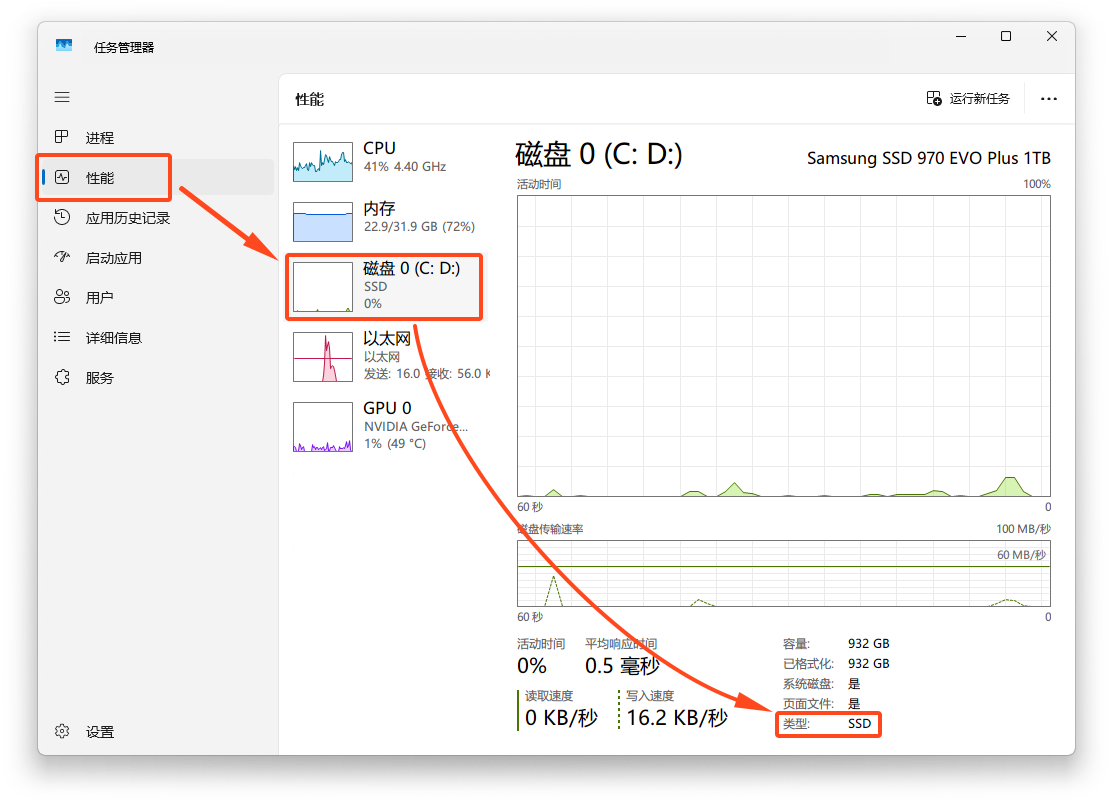
\includegraphics[width=.65\textwidth]{assets/basic/Check_disk_status.png}
  \caption{在任务管理器看看硬盘}
  \label{fig:Check_disk_status}
\end{figure}

打开「任务管理器」,切换到【性能】选项卡,其中【磁盘 0】【磁盘 1】就是一块块硬盘,其后的括号内则列出了该硬盘上的分区。点击一块硬盘,可以看到它的大小和类型(机械硬盘 HDD、固态硬盘 SSD)等信息。

\subsection{显卡(GPU)}

如果你是喜欢玩游戏的读者,「显卡」将是你在选购电脑时需要着重考虑的一个因素。

以前,「显卡」就是电脑里面的一个独立的模块,像一张卡一样插接在主板上。这个模块的功能是专门进行画面的绘制和图像的处理,因而得名「显卡」。所有显示在屏幕上的画面,都是由显卡绘制的。因而,\regcolor{显卡的好坏对游戏和图形相关的工作(比如三维制图、视频编辑)有较大影响}。下图展示了一块老旧的电脑显卡,其中 ➊ 是用于连接显示器的端口,➋ 处则是与电脑主板连接的触点。➌ 为这块显卡的散热风扇,而在其下方压着的 ➍,就是显卡的核心部分——图形处理器(Graphics Processing Unit,简称 GPU)。

\begin{figure}[htb!]
  \centering
  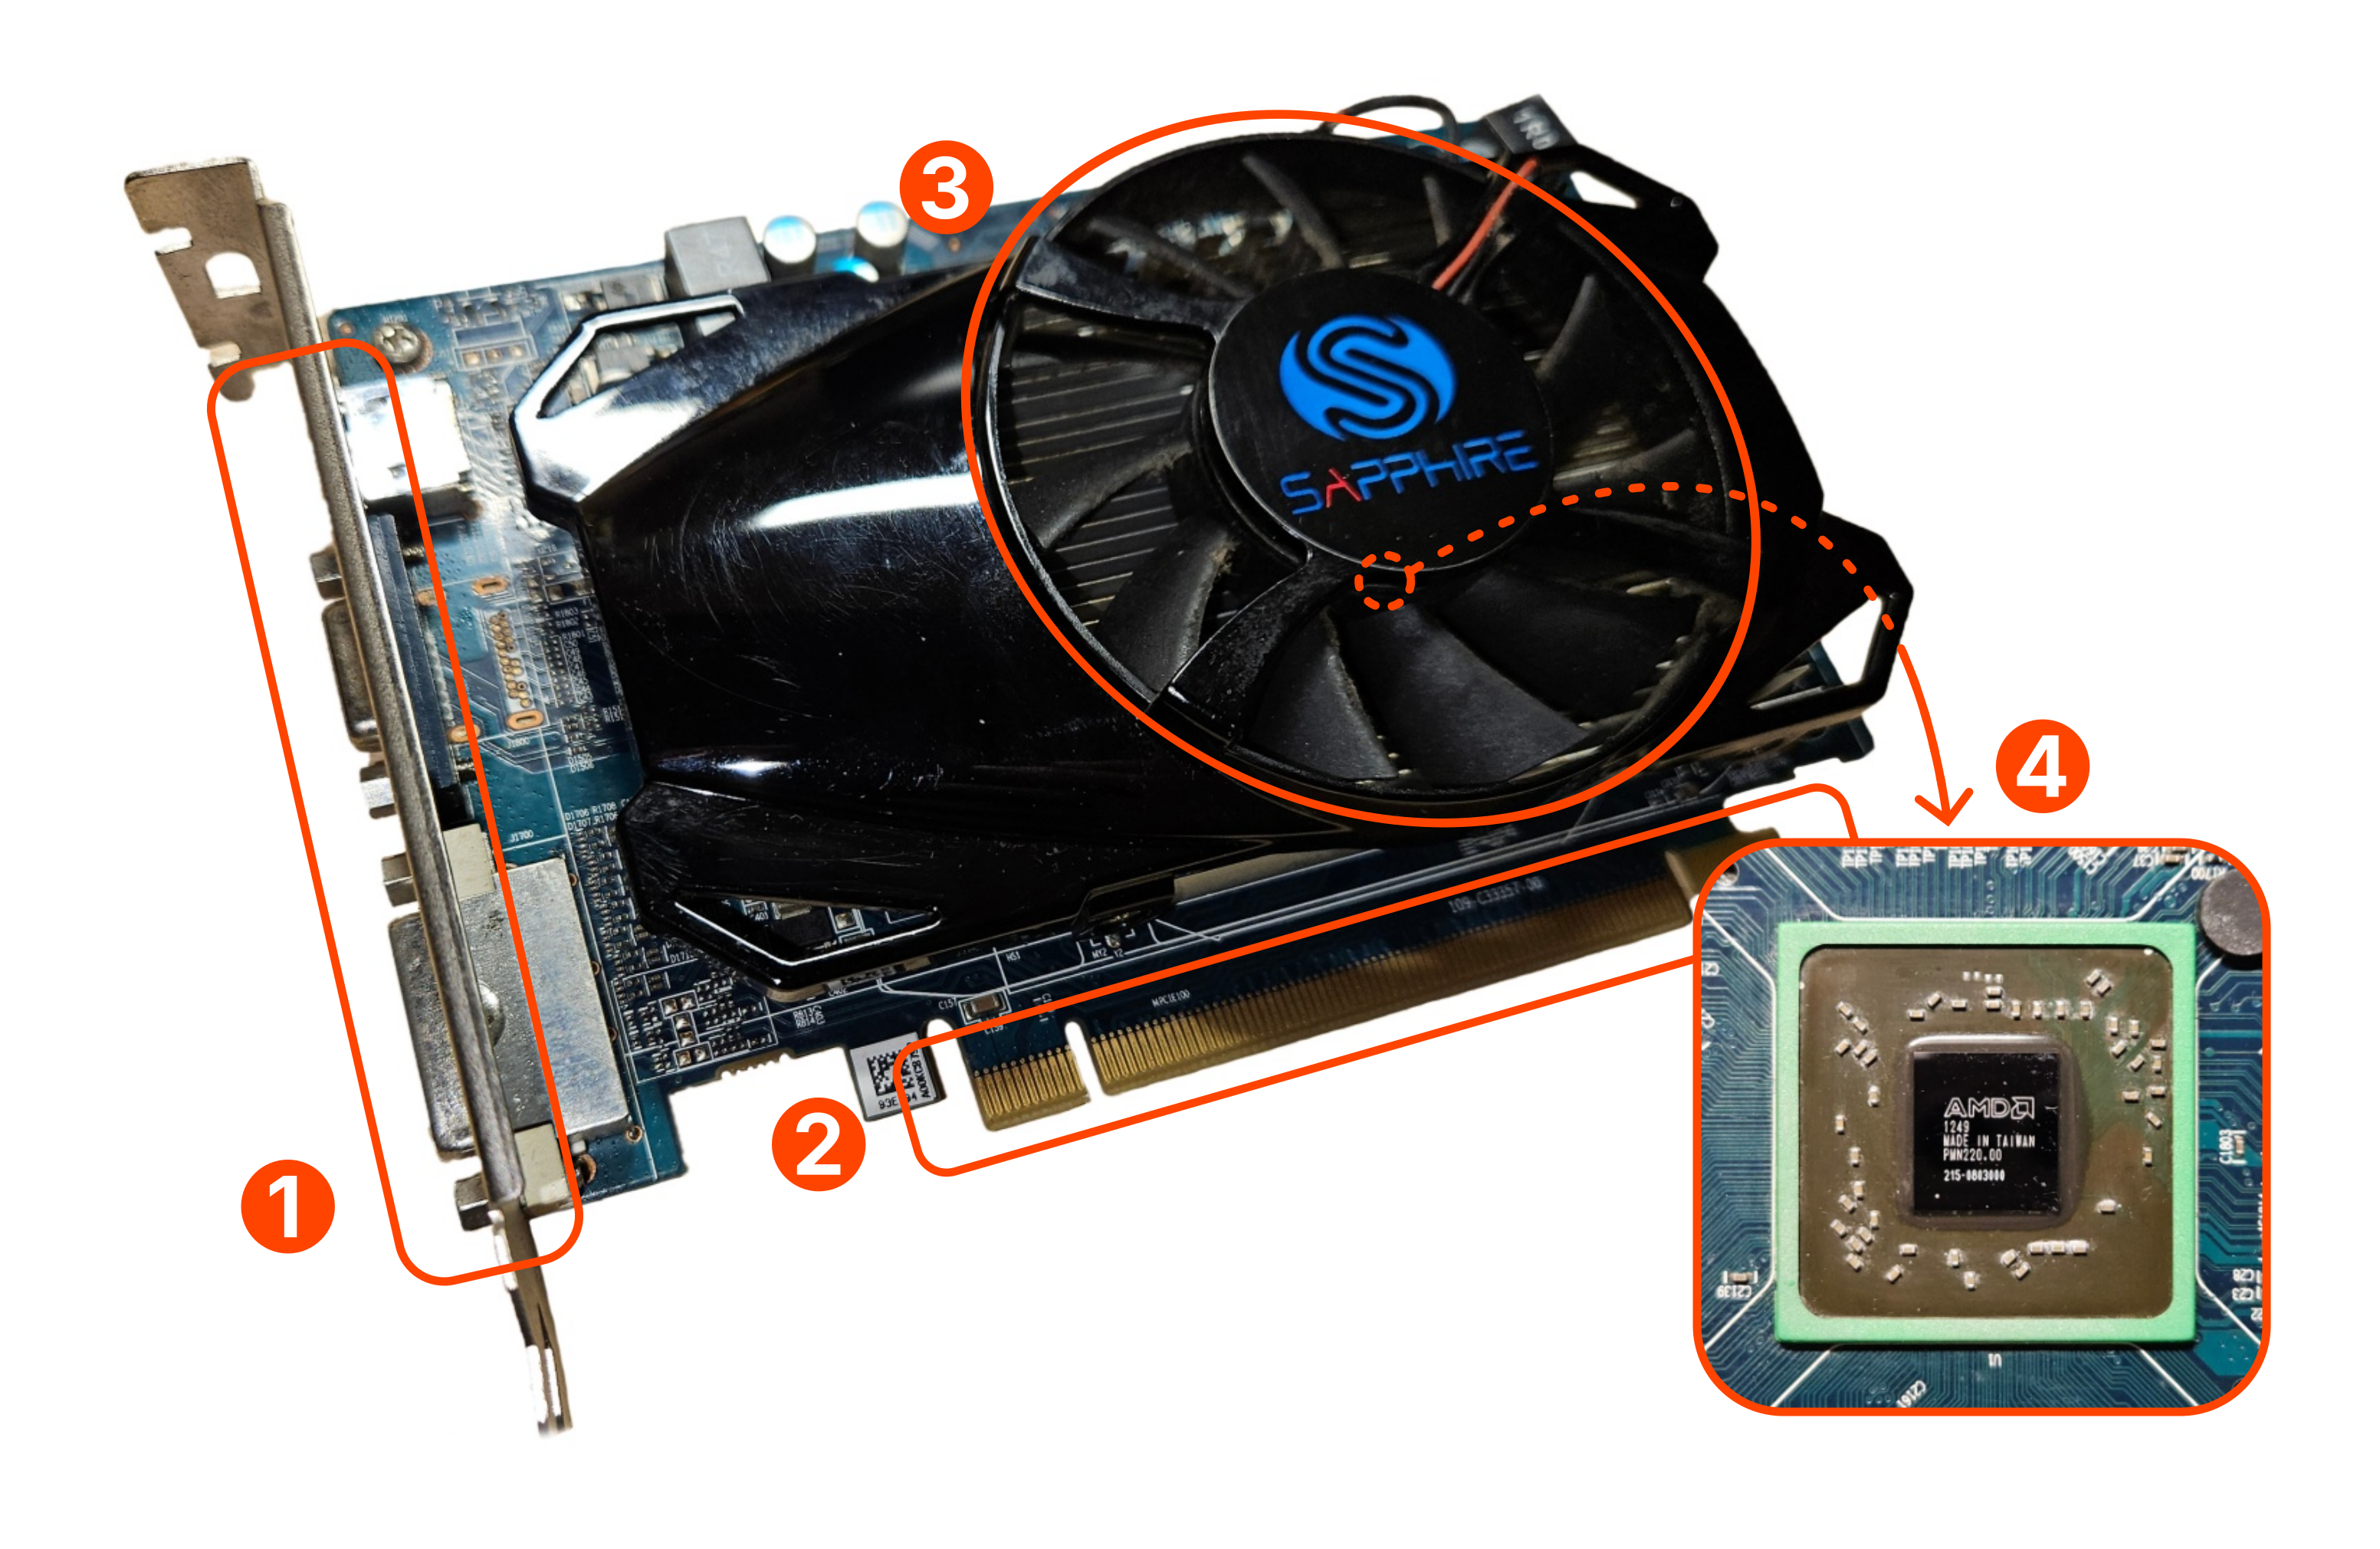
\includegraphics[width=8cm]{assets/basic/GPU_parts.png}
  \caption{老显卡(也是现在显卡)的各部分}
  \label{fig:GPU_parts}
\end{figure}

\begin{note}
  也就是说,GPU 是一枚芯片,而显卡是承载着这个芯片的模块。不过现在,人们习惯于将这两个词混用——既可以用「GPU」代指整个显卡,也可以用「显卡」或「显卡芯片」一词来特指 GPU 那枚芯片。强求区分它们显得有点古板学究气了,因此在本书中,我们也会混合使用两种称呼。
\end{note}

为什么上面那段要加上「以前」两个字呢?因为随着半导体技术的发展,人们后来发现,GPU 可以「集成」到处理器\footnote{一开始,集成显卡并不是集成到处理器中的,而是集成在主板上的一个芯片之中(称为「北桥」),后来才集成到了处理器里面。}中,换言之,就像多核处理器把几个核心放在一个芯片上一样,GPU 也可以和 CPU 做成一块芯片。容易想到,这样集成到一起之后,受限于芯片整体的大小,GPU 不能做得性能很强了:CPU 就在它边上,与它一起发热,一起分享能量。但是,通过这种方式,可以有效缩小硬件的体积,也能降低功耗。因而,发展到今天,GPU 在电脑中的形态有了以下两种:

\begin{itemize}
  \item \regcolor{集成显卡},简称「\regcolor{集显}」,又称「\regcolor{核显}」,英特尔称「核芯显卡」,AMD 则将 GPU 和 CPU 构成的整体一同称为「APU」。GPU 被安排在处理器的同一片芯片上,性能相对较差,能应付大多数工作,但游戏、制图等特定工作就不太行了。集成显卡功耗很低,而且省去了用户单独购买显卡的麻烦。
  \item \regcolor{独立显卡},简称「\regcolor{独显}」。GPU 仍然是一片独立的芯片,以显卡模块的形式安装在电脑内。这样的 GPU 性能较强,但换来的是更高的功耗、更大的体积和更多的发热等。如果你喜欢玩游戏(尤其是大型 3D 游戏),又或者从事视频编辑、三维设计等工作,那么一台装有独立显卡的电脑可能是你的刚需。
\end{itemize}

今天,全世界生产\regcolor{独立显卡}的厂商主要有两家,一家叫「英伟达」(NVIDIA),它旗下的显卡俗称「N 卡」;另一家则是前文提到过的 AMD,它推出的显卡俗称「A 卡」。如果你有涉足过游戏交流圈,玩家所说的「RTX 4090」「GTX 1080 Ti」等都是英伟达显卡的型号,而「RX 6800 XT」「RX 580」等都是 AMD 显卡的型号。下图是英伟达网站上出售的\CJKsout*{《黑神话·悟空》联名款的} RTX 4070 Super 高端显卡,可以看到显卡上有三个大尺寸的散热风扇,这从侧面说明其功耗之大、发热之多。

\begin{figure}[htb!]
  \centering
  
\includegraphics[width=.6\textwidth]{assets/basic/4070_storepage.png}
  \caption{在售的RTX 4070 Super}
  \label{fig:4070_storepage}
\end{figure}

\begin{note}
  除了英伟达和 AMD 之外,市面上也有一些其他品牌的独立显卡。或许来源于在集成显卡设计上的经验,英特尔也推出了自己的独立显卡系列。同时,我国公司「摩尔线程」也率先推出了面向民用市场的国产显卡,具有比较优秀的理论性能。然而,由于市面上的游戏、软件大都主要针对英伟达和 AMD 显卡进行设计、优化,摩尔线程显卡的实际体验目前还有许多的提升空间。
\end{note}

一般来说,对于笔记本电脑,轻薄本大都使用集成显卡,而游戏本大都装配有独立显卡。显然,这是由它们的使用场景和目标人群不同所决定的。不过,因为笔记本电脑内部空间相当有限,笔记本内即使装配了独立显卡,它们的性能也要比同级别的台式机独立显卡要差。同时,笔记本的独立显卡往往不是「插」而是「焊」在主板上的,我们几乎不可能对它们进行更换、升级,更别说给没有独立显卡的笔记本电脑加装一块独显\footnote{不过,如果你的笔记本电脑配有「雷电 3」「雷电 4」或「OCuLink」等接口,你可以通过这个接口连接外置的独立显卡来使用,但是这样做并不十分方便,受众并不多。}。

我们可以把 GPU 的任务理解成「根据 CPU 的命令,画出图形并输出到显示器上」。为了完成这个任务,\regcolor{GPU 拥有属于自己的内存,称为「显存」}。GPU 使用显存空间来暂时存放它正在绘制的画面,同时还要存放大量与图形有关的其他内容。这使得显存的大小成为了决定(独立)显卡性能和价格的一个重要因素。目前,高端的独立显卡拥有 10 GB 甚至 20 GB 以上的显存,这使得它们得以从容应对各种复杂的游戏画面。而至于集成显卡,它们则需要从电脑内存中「借」一部分空间充当显存,因此更难以应付大量的图形工作。

值得注意的是,近些年来,随着人工智能(AI)技术的发展,GPU 的功能已经不再局限于「打游戏」「制图」等图形工作——\regcolor{在 AI 模型的训练和推理过程中,GPU 的并行计算能力能提供比处理器更好的性能},同时独立显卡的显存还能提供比电脑内存更快的访问速度。如果你了解过 AI 绘画或 AI 作曲等技术,在它们的说明文档中,你一定会看到对 GPU 的需求。若你对这方面有兴趣,那么 GPU 的性能,尤其是显存的大小,就成了你选购电脑时的重要考虑因素。

\begin{note}
  想了解和 AI 有关的更多知识?没问题!请看超越篇的\nameref{cha:bring-intelligence-to-machines}。
\end{note}

在任务管理器中,我们同样可以看到有关显卡的信息:在【性能】页面左侧的列表末尾,【GPU 0】【GPU 1】等就表示着我们电脑上的一张张显卡。

\section{与我们「打交道」的软件}

\subsection{软件与操作系统}

由处理器、内存、硬盘以及各种各样的外围电子元件,共同构成了一台电脑的硬件部分。而在硬件之上,具体的工作任务是由软件来指派的。

我们可以用每天都在用的手机来理解:\regcolor{手机上,无论是我们自己安装的「QQ」「微信」「网易云音乐」,还是手机预置的「电话」「短信」,都属于「软件」}。「QQ」「微信」指挥硬件去利用网络收发信息,利用屏幕展示数据;「网易云音乐」指挥硬件去播放声音,同时在屏幕上展示评论;「电话」「短信」指挥硬件利用无线电模块发送和接收信号……同样一部手机,硬件还是那个硬件,但能通过不同的软件行使不同的具体功能。

而在「QQ」「微信」「电话」等 app 和纯粹的硬件之间,有\regcolor{一个更大,而且更「底层」的软件,称为「操作系统」}。简单地说,操作系统「夹」在各软件和硬件之间,为软件具体行使功能提供了一系列方便的「接口」。有了操作系统,网易云音乐 app 不再需要真正地去想「怎么让喇叭发声」,而只需要考虑「怎么告诉操作系统让喇叭发声」。「让喇叭发声」是一个带些复杂物理知识的过程,但「告诉操作系统让喇叭发声」则相对简单得多。

\begin{figure}[htb!]
  \centering
  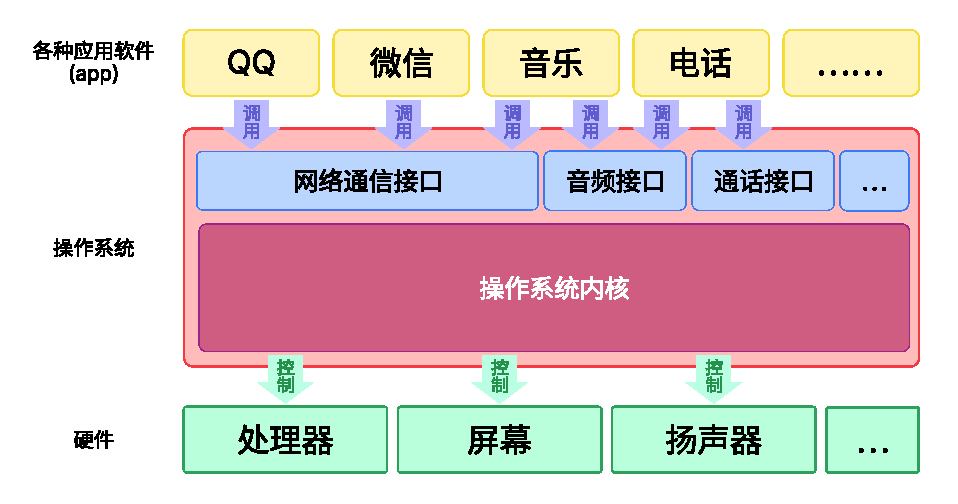
\includegraphics[width=.8\textwidth]{assets/basic/OS_structure.pdf}
  \caption{App、操作系统和硬件的关系}
  \label{fig:OS_structure}
\end{figure}

\begin{note}
  尽管操作系统是一个特殊的软件,但在日常生活中,「软件」一词通常只指微信、QQ 或是 Word、PowerPoint 等「应用软件」,即 app。在本书中,除非特别说明,「软件」和「app」是相同的含义,我们会混合使用它们。
\end{note}

由于上层的软件需要依赖操作系统来实现功能,而每个操作系统留给软件的接口细节上也有所不同,因此,\regcolor{针对不同操作系统开发的软件是不能直接通用的}。软件厂商一般会为不同的操作系统开发同一款软件,这样就能照顾到使用不同系统的用户。

今天,主流的手机操作系统有「安卓」(Android)、「iOS」以及「鸿蒙」(Harmony OS)。安卓系统是开放的,因此被各个手机厂商广泛使用,而 iOS 和鸿蒙目前则分别用在苹果和华为的设备上。如果你在网上下载过手机 app,一定会注意到厂商要根据操作系统提供不同的下载入口,这正是因为不同系统上的软件相互不兼容。

而在电脑上,「Windows」「Linux」及「macOS」是最常见的三种操作系统。\regcolor{Windows 最为普遍,几乎所有的个人电脑都运行着 Windows 系统}。Linux 是一种开源的操作系统,主要在服务器上使用,一些专业人士也会在日常使用;macOS 则是苹果推出的电脑操作系统,理论上只能用于苹果的电脑。下图中,(a) 至 (c) 依次是 Windows 11、Linux(使用 GNOME 桌面环境)和 macOS Sonoma 的界面。

\begin{figure}[htb!]
  \centering
  \includegraphics[width=.8\textwidth]{assets/basic/Three_systems.pdf}
  \caption{三大主流电脑操作系统}
  \label{fig:Three_systems}
\end{figure}

\subsection{Windows 操作系统}

我们绝大多数人都在使用 Windows 操作系统,《你缺计课》亦是一套基于 Windows 的电脑教程。所谓「Windows XP」「Windows 7」和「Windows 10」则是 Windows 操作系统的不同版本。

Windows 由美国的微软公司所开发,诞生于 1985 年。到今天(2024 年),Windows 已经经历了数个大版本的更新\footnote{关于 Windows 的一点点更新历史,可以参见“\nameref{cha:recover-from-bsod}”一章。}。今天,除了苹果以外几乎所有品牌的个人电脑都运行着 Windows 系统。目前最新的 Windows 版本是 Windows 11(发布于 2021 年 10 月 5 日),它与 Windows 10(发布于 2015 年 7 月 29 日)一同占领了大部分电脑。在有些地方,一些稍旧的计算机运行着 Windows 7,而更老的 Windows 版本(如 Windows XP)目前已经鲜有使用。不同版本 Windows 系统之间会有操作细节、使用体验上的不同,不过往往最直观的不同是它们的外观。下图中,(a) 和 (b) 分别展示了 Windows 11 和 Windows 10 的界面。

\begin{figure}[htb!]
  \centering
  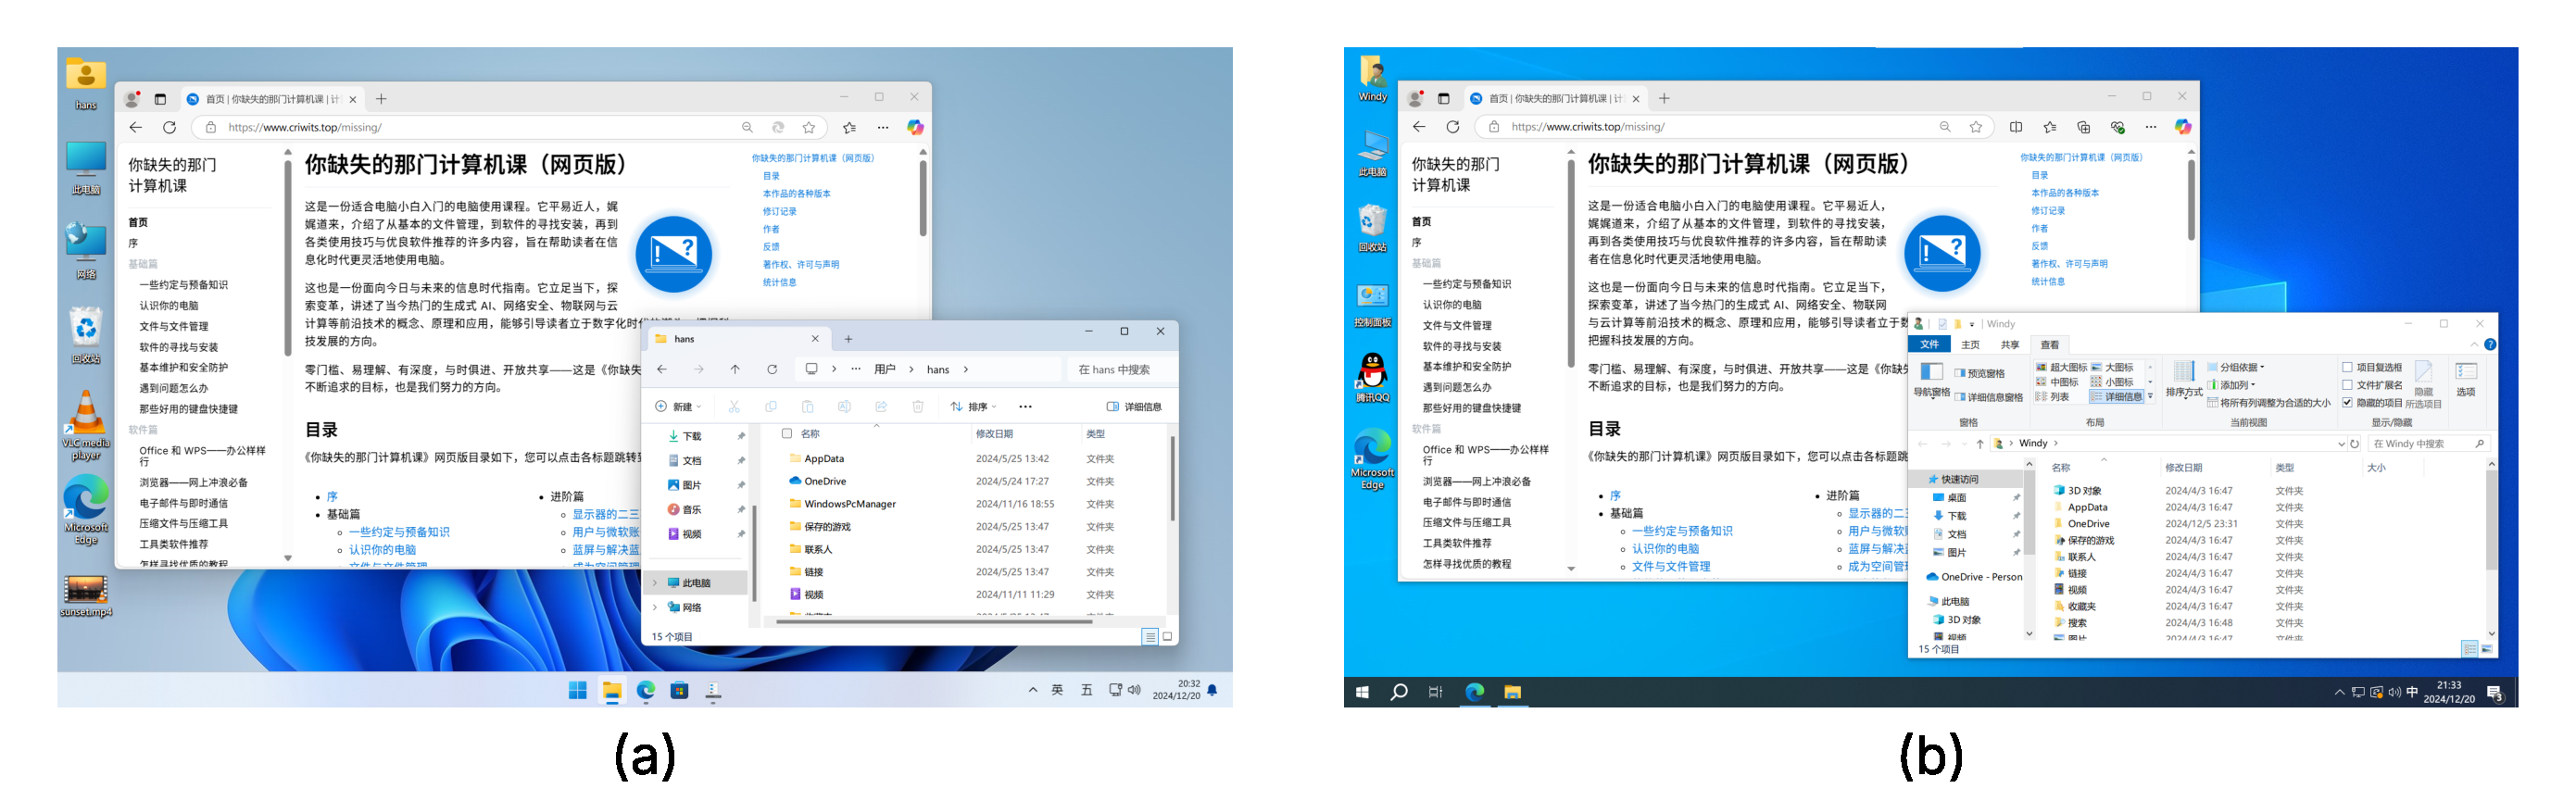
\includegraphics[width=.9\textwidth]{assets/basic/Win_11_and_10.pdf}
  \caption{如今的两大Windows}
  \label{fig:Win_11_and_10}
\end{figure}

通过右键桌面上的【此电脑】并点选【属性】,或打开系统设置,选择【系统】→【系统信息】(Windows 10 则是【关于】),你可以看到自己电脑 Windows 系统的版本。

\begin{figure}[htb!]
  \centering
  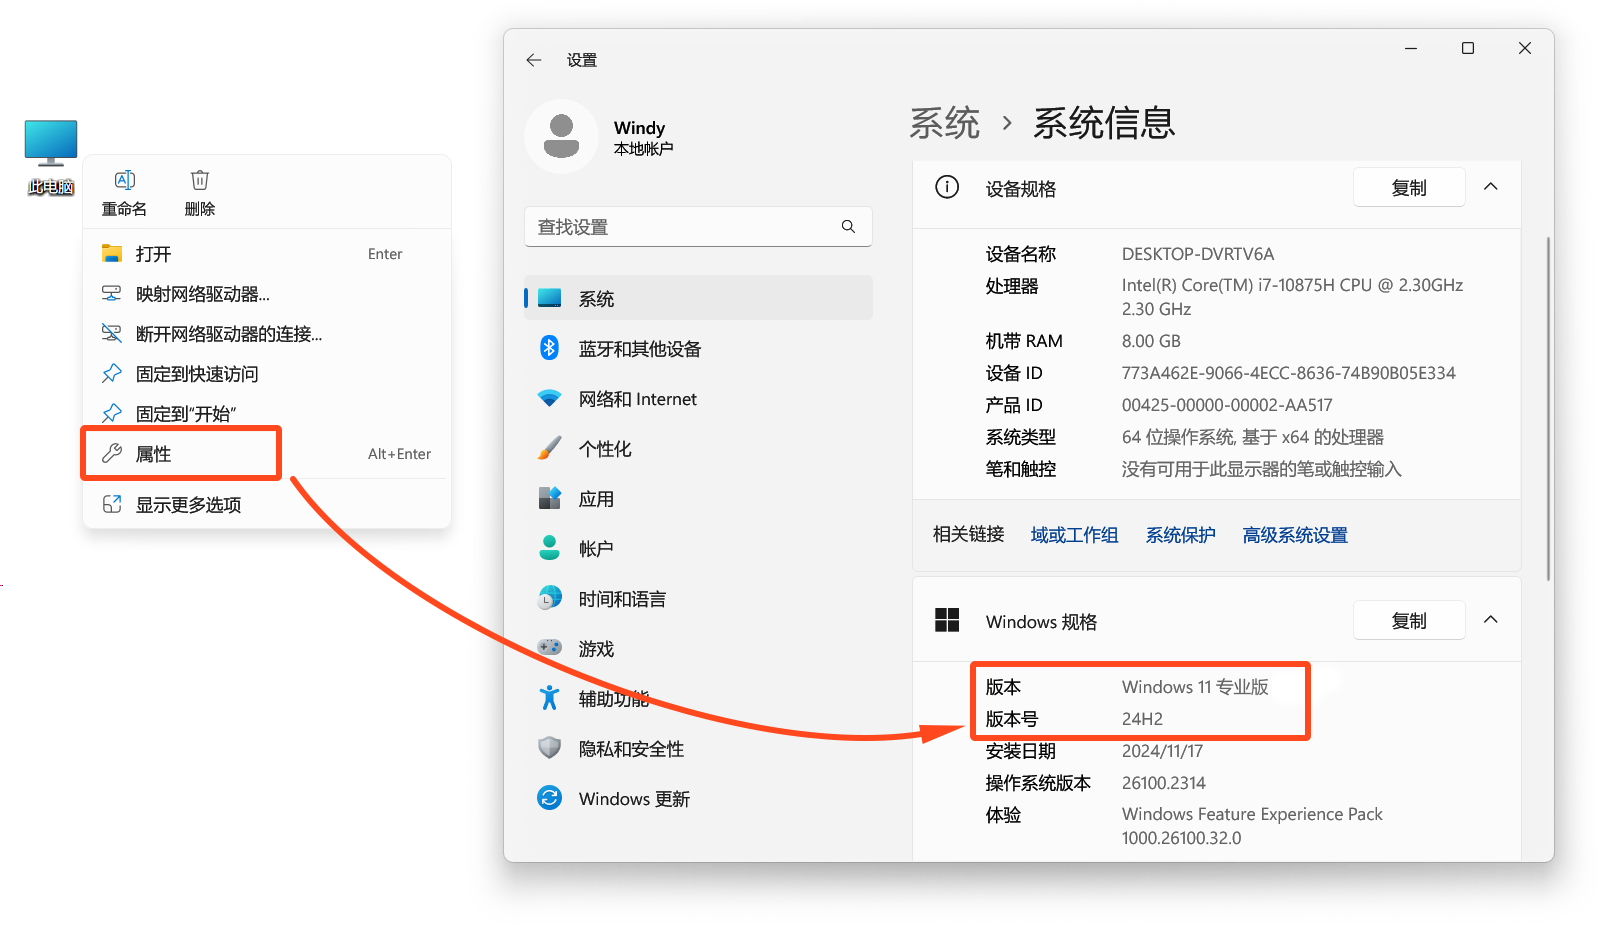
\includegraphics[width=.7\textwidth]{assets/basic/Check_Windows_version.png}
  \caption{检查 Windows 系统版本}
  \label{fig:check-windows-version}
\end{figure}

\regcolor{本书假定读者使用的系统是 Windows 11 或者 Windows 10,其中所有的操作都是基于 Windows 11 或者 Windows 10 简体中文版系统来描述的。}不过,本书所介绍的知识是通用的,如果你使用的是 Windows 7、Windows 8 或者 Windows 8.1,本书提到的多数操作你也能正常使用。一些明确仅能用于 Windows 10 和/或 Windows 11 的操作和技巧一般会特别标注。

\practice

\begin{enumerate}
  \item 通过任务管理器和【此电脑】→【属性】,查看自己电脑的 Windows 版本、CPU 型号和核心数、内存大小、硬盘大小和类型、显卡大小和类型。
  \item 你使用的是游戏本还是轻薄本?亦或是介于二者之间的所谓「全能本」?尝试翻到笔记本的底面,上网搜索它底面所写的型号,了解关于你自己机器的更多信息。
  \item 你对「电路」的认知有多少?你是否好奇 CPU 是怎么运作的?从开关、导线、电池、灯泡组成的最简单「电路」到几乎无所不能「电脑」之间到底发生了什么奇妙的变化?在本书超越篇的\nameref{cha:program-and-arch}一章中,我们会简要向你进一步介绍这些问题。但限于《你缺计课》篇幅,我们是没法完全告诉你这些的。但是,你若有兴趣,可以去学习「电路电子技术」「计算机体系结构」「计算光刻」「纳米测量技术」等相关内容。近年来,国际形势风云变幻,我国在芯片领域仍然存在许多短板。我们希望越来越多的有志青年能投身于包括但不限于体系结构、硬件组成、数字电路乃至微电子、集成电路制造、半导体材料等领域,为我国芯片行业「补上短板」贡献自己的力量。
\end{enumerate}

\chapter{文件与文件管理}
\label{files-and-file-management}

\begin{intro}
  在这一部分,我们将重新介绍你可能所不知道的「文件」以及「文件」的管理,以及一些实用的文件管理的技巧。
  看完这一部分,你将可以找到下面这些问题的答案:
  \begin{itemize}
    \item 为什么很多人说「不建议把文件放在桌面上」?
    \item C 盘总是「红了」,为什么?为什么有人建议把软件装到 D 盘里?
    \item 「扩展名」是什么?「打开方式」又是什么?为什么有时候我电脑上的 Word 文档就打不开了?
  \end{itemize}
\end{intro}

如上一章所言,硬盘是电脑中存放数据的地方,而「文件」则是数据存放的具体形式。
你所撰写的 Word 文档、制作的 PPT 幻灯片、从网上下载的图片,乃至各个 app 或者说软件本身,都以文件的形式存储在硬盘上。

这一部分,我们将具体介绍「文件」和文件的管理。
这是《Missing》需要动手实践的第一章,也是我们合理、有效地使用电脑的第一课。

\section{硬盘的分区}

打开桌面上的【此电脑】(但其实打开的东西叫「文件资源管理器」),我们往往可以看到多于一个的「盘」,例如 C 盘、D 盘等。
这样的「盘」学名叫做「分区」,顾名思义,它们是将硬盘上的空间人为地划分成了一些子空间。

\begin{figure}[htb!]
  \centering
  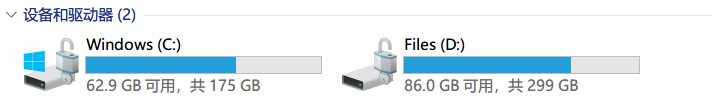
\includegraphics[width=13cm]{assets/Hans_Disks.jpg}
  \caption{Hans 电脑上的分区}
  \label{Hans_Disks}
\end{figure}

例如,上图是 Hans 的笔记本电脑「此电脑」中的分区。
可以看到,这两个分区一个大小为 175 GB,另一个大小为 299 GB,相加为 474 GB——这是这台电脑的硬盘可用总空间。

划分分区的意义,在于帮助我们更好地管理文件。
分区划分之后,各个分区之间就仿佛被「隔离」开来了,如图 \ref{Disk_Parts} 所展示的那样。
即使我们「格式化」一个分区(这样会删除这个分区中的所有文件),也不会影响另外一个分区里面的文件。

\begin{figure}[htb!]
  \centering
  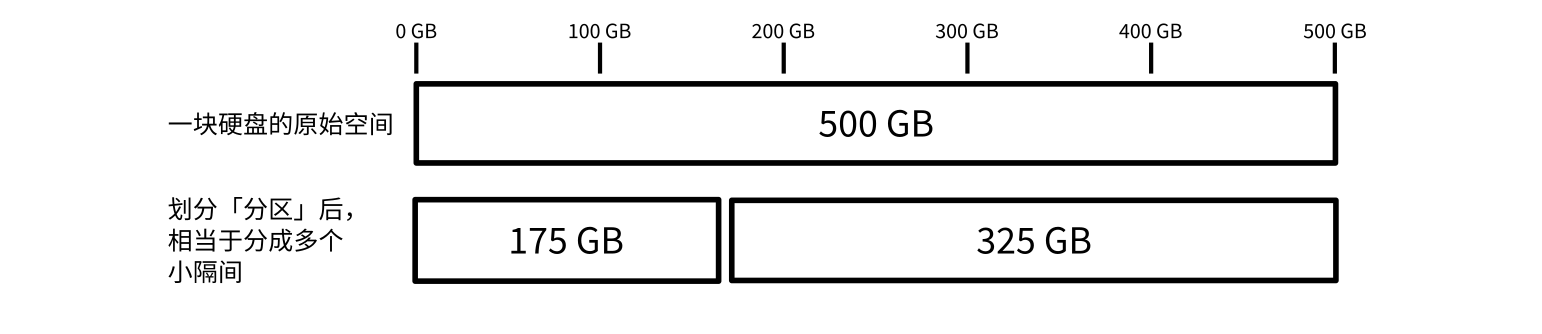
\includegraphics[width=.9\textwidth]{assets/Disk_Parts.png}
  \caption{硬盘与分区的关系}
  \label{Disk_Parts}
\end{figure}

在 Windows 系统中,分区会被给予两个标识符,或者说「名字」:

\begin{itemize}
  \item 一个是「\regcolor{盘符}」,盘符是一个英文字母加上冒号 \verb|:| 构成的。
    我们所称呼的「C 盘」「D 盘」正是指盘符中的那个字母。
    如上图,左方分区的盘符是 \verb|C:| ,右方分区的盘符是 \verb|D:| 。
    盘符一般在被指定之后就不方便更换了。在今天,Windows 系统中的盘符都是从字母 C 开始\footnote{这是因为 A 和 B 两个盘符在过去是留给「软盘」的,但软盘早就已经成为历史了,不过这个习惯却保留了下来。}的。
  \item 另一个是「\regcolor{卷标}」,这是一个可选的标识符,它是一定长度的文本。
    在上图中,C 盘的卷标是「Windows」,D 盘的卷标是「Files」。
    盘符的作用是让系统和软件识别分区,而卷标的作用是帮助我们用户更加直观地了解分区的作用,因而卷标是可以随时更换的。
    事实上,通过右键某一分区,选择【重命名】,就可以更换卷标了。如果你什么都不写,它默认叫做「本地磁盘」。
\end{itemize}

\begin{figure}[htb!]
  \centering
  
\includegraphics[width=7cm]{assets/Volume_Name_and_Letter.jpg}
  \caption{盘符与卷标}
  \label{Volume_Name_and_Letter}
\end{figure}

我们在\nameref{computer-and-its-components}中提到,操作系统本身也是一个大软件,那么这个软件放在硬盘上的哪呢?
对于 Windows 而言,整个 Windows 系统默认放在 C 盘里。
双击打开电脑 C 盘,你会看到一些你可能不熟悉的文件夹,例如 \verb|Windows| 文件夹,Windows 系统自己的许多文件就存在其中。

也许你听过「不要把软件安装到 C 盘」这样的说法。这是有根据的。
系统本身就已经很庞大,系统自身工作产生的一些文件也会被自动地放在 C 盘内,导致 C 盘本身空间就容易变得局促。
如果还将大量的软件装在 C 盘,会让 C 盘更加「不堪重负」,结果就是——红了。

在本章的后续部分,以及\nameref{software-installation}中,我们会详细介绍,怎样把我们的软件以及其他东西放在 C 盘以外的地方,以及这样做的其他好处。

\section{文件、文件名和文件类型}

「文件」是数据存储在硬盘上的形式。这么说可能有些抽象,直观地说,文件就是我们每天都打交道的东西:

\begin{figure}[htb!]
  \centering
  
\includegraphics[width=7cm]{assets/Files.jpg}
  \caption{一些文件}
  \label{Files}
\end{figure}

文件有自己的「名字」,称为「文件名」。
在 Windows 系统中,文件名可以分成三个部分:

\begin{itemize}
  \item 「主名」是指文件名中,点号 \verb|.| 之前的部分。
    这部分内容可以自定,相当于人类的姓名。
    上图中,「 \verb|如何让富婆爱上我| 」和「 \verb|一夜暴富指南| 」等都是文件的主名。
  \item 「点号」是指文件名中间的那个「 \verb|.| 」。
  \item 「扩展名」是指文件名中,点号「 \verb|.| 」之后的部分\footnote{有时候我们称呼文件的扩展名时也会把点号包含进去。下面两种说法是等价的:
      \begin{itemize}
        \item 某文件的扩展名是\texttt{txt}。
        \item 某文件的扩展名是\texttt{.txt}。
      \end{itemize}}。
    扩展名展示着文件的类型,它会告诉操作系统,这个文件应该用什么方式来打开。
    例如,上图中「 \verb|每天一个长寿秘诀.txt| 」中的「 \verb|txt| 」就是这个文件的扩展名,它说明这个文件是一个「文本文档」,应该使用「记事本」打开。
\end{itemize}

\begin{figure}[htb!]
  \centering
  \begin{minipage}{.48\textwidth}
    \centering
    
\includegraphics[width=.95\textwidth]{assets/File_Name.png}
    \caption{文件名结构}
    \label{File_Name}
  \end{minipage}
  \begin{minipage}{.48\textwidth}
    \centering
    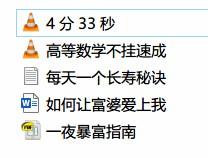
\includegraphics[width=.95\textwidth]{assets/Files_No_Ext.jpg}
    \caption{没有显示扩展名的文件}
    \label{File_No_Ext}
  \end{minipage}
\end{figure}

扩展名也是可以人为改变的,但这样往往会出问题——试想,对于上图中的 \texttt{高等数学不挂速成.mp4} ,它本来是一个 \verb|mp4| 文件,即「视频文件」,应该用看视频的软件打开。
如果你强行把它改成 \verb|txt| ,系统就会用「记事本」来打开一个「视频文件」——用错误的工具打开文件。

如果你的电脑上,文件的扩展名没有被显示(也就是说你只能看到文件的主名),如图 \ref{File_No_Ext} 所示。
在 Windows 10 中请点选文件夹窗口上方的【查看】选项卡,然后勾选【文件扩展名】,如图 \ref{Windows_10_set_full_filename} 所示;在 Windows 11 中请点选文件夹窗口上方的【查看】菜单,然后勾选【显示】→【文件扩展名】,如图 \ref{Windows_11_set_full_filename} 所示。

\begin{figure}[htb!]
  \centering
  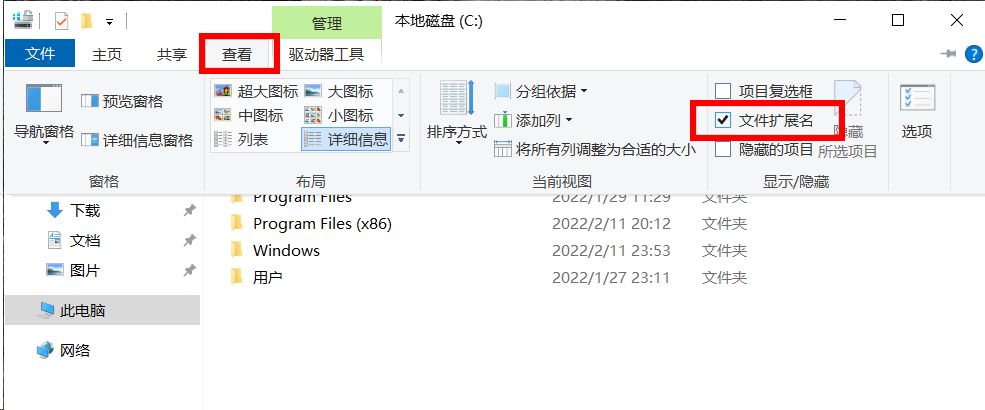
\includegraphics[width=10cm]{assets/Windows_10_set_full_filename.png}
  \caption{Windows 10 设置方法}
  \label{Windows_10_set_full_filename}
\end{figure}

\begin{figure}[htb!]
  \centering
  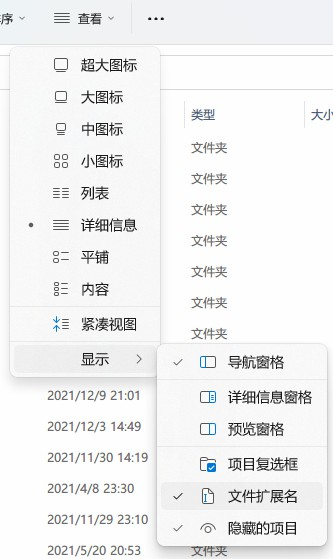
\includegraphics[width=4cm]{assets/Windows_11_set_full_filename.jpg}
  \caption{Windows 11 设置方法}
  \label{Windows_11_set_full_filename}
\end{figure}

在打开这个选项之后,文件扩展名不仅是可见的,甚至是可以改变的——但如上文所说,扩展名不能随便改,因为改了之后系统就会用错误的工具去打开它。
右键某一文件,选择【重命名】,你会看到系统会自动帮你选中文件的「主名」,而不选中「扩展名」。
如果你执意更改文件的「扩展名」,系统会发出一个提示:

\begin{figure}[htb!]
  \centering
  
\includegraphics[width=6cm]{assets/Warning_of_Changing_Ext.jpg}
  \caption{尝试更改扩展名……}
  \label{Warning_of_Changing_Ext}
\end{figure}

「那既然这样,我不想不小心突然间改掉文件的扩展名,还不如不开呢。」如果你有这样的想法,那么另一重危险正悄然降临。且看下面的两个文件:

\begin{figure}[htb!]
  \centering
  \begin{minipage}{.48\textwidth}
    \centering
    
\includegraphics[width=.95\textwidth]{assets/fake_doc.png}
    \caption{两个神奇的文件}
    \label{fake_doc}
  \end{minipage}
  \begin{minipage}{.48\textwidth}
    \centering
    
\includegraphics[width=.95\textwidth]{assets/fake_doc_revealed.png}
    \caption{揭示扩展名后}
    \label{fake_doc_revealed}
  \end{minipage}
\end{figure}

这两个「高数速成秘籍」看起来完全一样,就是两个正常的 Word 文档,但众所周知,一个目录下不可能存在两个文件名相同的文件,显然这里面必然有猫腻。
现在打开文件扩展名,这两个文件的名称变成了下面这个样子,可见,其中一个居然是可执行文件(\verb|exe|)格式,即一个应用程序(详见下文),只是图标故意被做成了 Word 文档的样子。
所以,看不到扩展名的话,指不定哪天有居心叵测的人发来一个这样伪装的病毒,那可就不好了。


\section{文件夹、路径和目录}

「文件夹」是一个用来存放其他文件的结构。
不妨想象一下现实中的「文件夹」:

\begin{figure}[htb!]
  \centering
  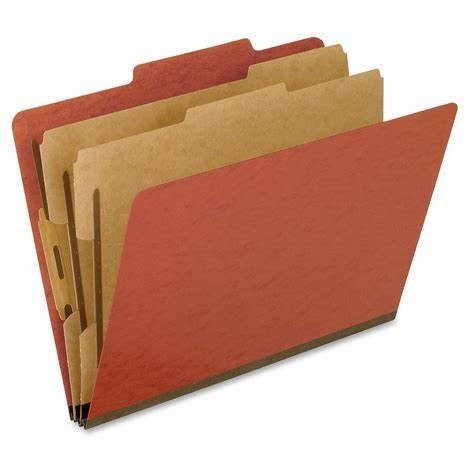
\includegraphics[width=4cm]{assets/Real_Folder.jpg}
  \caption{真实的文件夹}
  \label{Real_Folder}
\end{figure}

在这样的一个「文件夹」中,可以放很多各类「文件」。
而电脑中的文件夹除了能放文件之外,还可以放很多的「子文件夹」,即「文件夹里面的文件夹」。
这个过程可以循环重复,因而一个文件夹的内部结构可以相当错综复杂。

如果抽象地把整个电脑看成一个巨大的「文件夹」,那么不同的分区就是这个巨大「文件夹」之下的几个子文件夹,我们的某一份文件就是在这些子文件夹之下的某一个角落里。
假设在 D 盘的 \verb|missing| 文件夹之中有一个叫做 \verb|源文件| 的子文件夹,在这个子文件夹中有一个文件叫 \verb|第三章.docx| ,我们用这种方式表示这个 \verb|第三章.docx| 文件在整个电脑中的位置:

\begin{verbatim}
  D:\missing\源文件\第三章.docx
\end{verbatim}

这一长串东西表示出 \verb|第三章.docx| 这个文件在电脑中的具体位置,我们把一长串东西称为 \verb|第三章.docx| 这个文件的「路径」(严格来说叫做「绝对路径」)。
不难发现,路径是从「分区」(也就是「盘」)开始,用反斜杠 \verb|\| 作为分隔,一级一级文件夹地展开,最后到具体的文件。
类似的,不只是文件,文件夹的路径也可以用这样的方式来表示,例如

\begin{verbatim}
  D:\missing\源文件
\end{verbatim}

表示的就是 \verb|源文件| 这个文件夹在电脑中的位置。
一个文件 / 文件夹的「路径」是唯一确定的;一个「路径」也能唯一确定一个文件 / 文件夹。

也许你有听说过「目录」这个名字。其实「目录」就是文件夹。
例如这个说法「打开目录 \verb|D:\missing\public\| 」 指的就是打开 D 盘中 \verb|missing| 文件夹里的 \verb|public| 文件夹。

目录(文件夹)一层一层的结构可以像图 \ref{Catalog_Tree} 一样从上到下画出来,称作「目录树」。
在目录树这种形式中,文件夹之间是「上下级」的关系,故「文件 A 在文件夹 B 中」也可以称作「文件 A 在文件夹 B 下」或者「A 在目录 B 下」甚至是「A 在 B 下」。
也就是说,「下」这个字就是「在……里」的意思。

\begin{figure}[htb!]
  \centering
  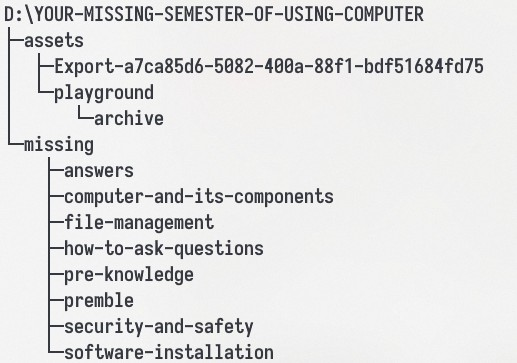
\includegraphics[width=8cm]{assets/Catalog_Tree.jpg}
  \caption{目录树}
  \label{Catalog_Tree}
\end{figure}

借助目录树这样的结构,我们就能理解「根目录」这个概念了。
一个盘的「根目录」指的是这个盘之下的第一级目录(恰好是目录「树」的「根」),例如 C 盘根目录就指的是路径 \verb|C:\| 。

\section{程序本身——可执行文件(\texttt{exe}文件)}

这一节我们介绍一种类型特殊的文件——「可执行文件」。
我们提到,数据是以文件的形式存储在硬盘上的,比如你所撰写的 Word 文档,它们都存储成了扩展名为 \verb|doc| 或者 \verb|docx| 的文件;
你所下载的图片,它们的扩展名则往往是 \verb|jpg| 、 \verb|jpg| 或者 \verb|gif| 。
而我们又提到,软件或者说 app 也是以文件的形式存储在硬盘上的。
那么,软件本身是什么格式的文件呢?

一个软件的核心是一个或多个「程序」,而程序是以「可执行文件」的形式存储的。
\regcolor{普通的文件,需要用其他的某个软件才能正常打开;而「可执行文件」双击就能运行自身,这就是「可执行」(Executable)的意思。}

可执行文件的扩展名是 \verb|exe| 。
对于这种类型的文件,系统不会想着用别的软件去打开它,而是直接运行它自身。
可执行文件有时被直接称为「程序文件」或者「程序」。

需要注意的是,电脑上的一款软件(或者说 app,在《Missing》中我们会同时使用这两种称呼)可能不仅仅只有一个程序,也就不止一个可执行文件。
下面是软件「网易云音乐」所在的文件夹中的一部分:

\begin{figure}[htb!]
  \centering
  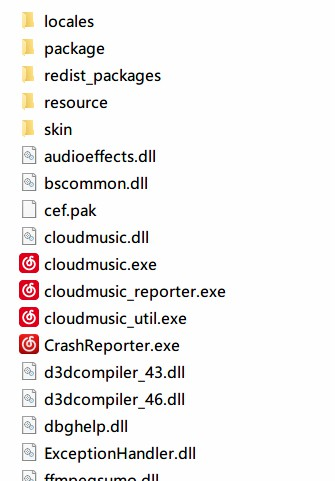
\includegraphics[width=5cm]{assets/NetEase_Music.jpg}
  \caption{网易云音乐的目录}
  \label{NetEase_Music}
\end{figure}

可以看到,「网易云音乐」这个 app 有着这些文件:

\begin{itemize}
  \item 可执行文件 \verb|cloudmusic.exe| ,这个是 app 的主体,即「网易云音乐」的主程序。
  \item 可执行文件 \verb|cloudmusic_reporter.exe| , \verb|cloudmusic_util.exe| 等。
    这些文件是 app 运行时的其他辅助程序,可以想象成乐队中主唱身边的吉他手 / 键盘手 / 鼓手 / 伴舞等。
    它们往往无法单独运行,而 \verb|cloudmusic.exe| 这个主文件脱离它们也不能运行。
  \item 一大堆的 \verb|dll| 和其他格式的文件。这些是 app 工作时不可或缺的依赖文件。
  \item 一些子文件夹,存储着 app 运行需要的另外一些东西。
\end{itemize}

每次我们启动「网易云音乐」,运行的都是 \verb|cloudmusic.exe| 这个可执行文件。
然而,这个文件的运行离不开放在它边上的那一堆辅助文件——如果你把 \verb|cloudmusic.exe| 复制到另外的一个地方,双击运行,大概率会直接报错;即使不报错,功能也必然有不正常。

在下一章我们在介绍软件的安装时会继续说明这个问题。

\section{文件的「替身」——快捷方式}

\begin{figure}[htb!]
  \centering
  
\includegraphics[width=10cm]{assets/Shortcut.png}
  \caption{快捷方式}
  \label{Shortcut}
\end{figure}

你是怎么启动「网易云音乐」的呢?

一般来说,我们会双击桌面上的「网易云音乐」或者点击开始菜单中的「网易云音乐」。
不管是桌面上的「网易云音乐」还是开始菜单里的「网易云音乐」,它们都是不是这个 app 本身——app 本身的样子我们在上面刚刚看过——而是另一种特殊类型的文件,称作「快捷方式」。

\begin{wrapfigure}[12]{r}{6cm}
  \centering
  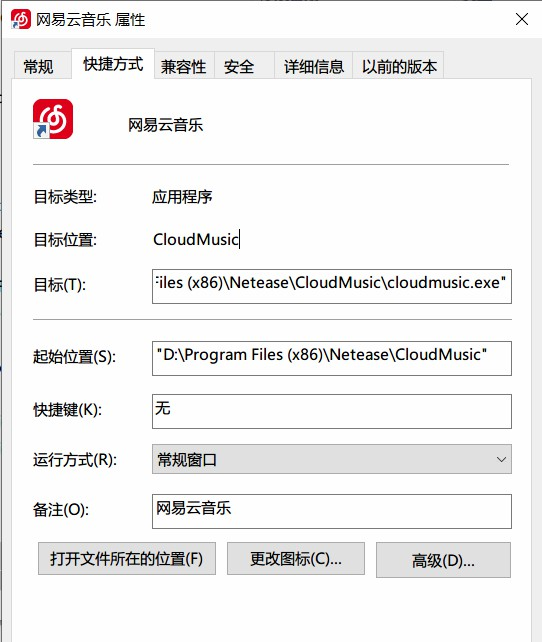
\includegraphics[width=5cm]{assets/NetEase_Music_Link.jpg}
  \caption{桌面上的「网易云音乐」}
  \label{NetEase_Music_Link}
\end{wrapfigure}

「快捷方式」可以看成某个具体文件的单向「指针」或者说「替身」,指向电脑某个角落里的某个文件。
它的扩展名是 \verb|lnk| ,但实际上不可见\footnote{千万不要手动把一个正常文件的扩展名改成\texttt{lnk},否则就很难改回来了。}。
你桌面上的「网易云音乐」,指向的正是网易云音乐软件目录下的那个 \verb|cloudmusic.exe| 文件。右击桌面上的【网易云音乐】,选择【属性】,会弹出这个快捷方式的详细信息:

其中「目标」一栏填写的正是 \verb|cloudmusic.exe| 这个可执行文件,即「网易云音乐」的主程序的路径:

\begin{verbatim}
  D:\Program Files (x86)\Netease\CloudMusic
  \cloudmusic.exe
\end{verbatim}

因此,你双击打开这个「网易云音乐」快捷方式,就会打开 \verb|cloudmusic.exe| 这个文件。
如果你\regcolor{删掉了这个快捷方式,它并不会影响 \texttt{cloudmusic.exe} 这个文件,不会影响你电脑上安装的网易云音乐本身。}

\begin{note}
  因此,卸载软件的方式可不是把桌面上的「快捷方式」删掉就完事的。
\end{note}

所有类型的文件以及文件夹都可以制作出无数个快捷方式。
如果你想给自己的某个文件 / 文件夹制作一个快捷方式,只需右键它,选择【发送到】→【桌面快捷方式】,就能在桌面生成一个指向这个文件的快捷方式了。
这个快捷方式可以挪到系统的任何地方,也可以复制粘贴出很多个副本。它们全都指向原来的那个文件本身。

一般来说,快捷方式的图标左下角会有一个「↗」符号。
这个符号标志着这个文件并非某文件本身而是一个快捷方式。

\section{合多为一,精简空间——压缩文件}

压缩文件并不是什么「特殊类型」的文件,但这里我们依然把它单独拿出来介绍。

压缩文件是利用一种特殊的软件「压缩软件」,将一批文件和文件夹「打包」而成的一种单个文件。
假设你有 8 个文件夹以及 7 个文件一共 15 个项目,你想一次性把它们分享给别人,那么把它们打包成一个压缩文件不失是一种好的选择。

\begin{figure}[htb!]
  \centering
  
\includegraphics[width=.9\textwidth]{assets/Compress.png}
  \caption{普通文件与压缩文件}
  \label{Compress}
\end{figure}

压缩文件有很多种类。最常用的是 \verb|zip| 文件和 \verb|rar| 文件,但后者的压缩软件是收费的\footnote{具体来说,大多数压缩工具都可以解压 \texttt{rar} 格式的压缩包,但只有 WinRAR 这一款压缩工具可以制作这种格式的压缩包;而这款工具是收费的。详见\nameref{archive-formats-and-tools}。}。
我们建议在与他人交换文件的时候,只使用 \verb|zip| 格式打包。

如果你电脑上已经安装有压缩软件,那么可以参照下面的方法将一批文件打包成一个压缩包:


\begin{itemize}
  \item 选中你要打包的文件。可以是一个文件 / 文件夹,也可以是一群文件 / 文件夹。
  \item 右击,选择【添加到压缩包】或者类似语义的选项。
  \item 设置参数,例如压缩格式(推荐 \verb|zip| 格式)、压缩后的文件的文件名以及压缩方式。\\
    一般来说,压缩后的文件的体积要比原来松散文件的体积小(所谓「压缩」)。
    具体而言,在压缩时可以选择「更快压缩」和「更小体积」之类的选项,前者压缩、解压都更快,但压缩时体积缩小得不明显;后者压缩、解压相对较慢,但压缩后体积可能缩小得更多。
  \item 开始压缩。压缩完成后,在原来的文件的相同目录下,就会生产一个 \verb|<文件名>.zip| 的文件。
\end{itemize}

如果收到一个压缩文件,我们一般需要将它解压。如果你电脑上已经安装有压缩软件,那么可以参照以下方法来解压缩:
右击压缩文件,选择【解压\footnote{部分压缩工具称「解压」为「提取」,是同一个词(Extract)的不同翻译。}到当前文件夹】或者【解压到 \verb|<文件名>\| 】。这两个选项的不同是:

\begin{itemize}
  \item 【解压到当前文件夹】会把压缩文件里的内容直接放在压缩文件的同一目录下。
    例如,如果一个压缩文件 \verb|archive.zip| 里面有 \verb|a.txt| 和 \verb|b.txt| 两个文件,选择此选项,解压后 \verb|a.txt| 和 \verb|b.txt| 都和 \verb|archive.zip| 在同一级目录。 
    \begin{figure}[htb!]
      \centering
      \begin{minipage}{6.2cm}
        \centering
        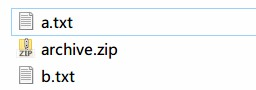
\includegraphics[width=6cm]{assets/Decompress_Current.jpg}
        \caption{【解压到当前文件夹】}
        \label{Decompress_Current}
      \end{minipage}
      \qquad
      \begin{minipage}{6.2cm}
        \centering
        
\includegraphics[width=6cm]{assets/Decompress_Sub.jpg}
        \caption{【解压到\texttt{<文件名>\textbackslash}】}
        \label{Decompress_Sub}
      \end{minipage}
    \end{figure}
  \item 【解压到 \verb|<文件名>\| 】会把压缩文件里的内容放在一个子文件夹里面。
    在上面的例子中选择这个选项,会在 \verb|archive.zip| 的同一级目录新建一个文件夹 \verb|archive| ,然后把 \verb|a.txt| 和 \verb|b.txt| 放在 \verb|archive| 文件夹下。
\end{itemize}

我们建议,为了不让自己的工作目录变得混乱,\regcolor{除非你知道自己这样做的原因,否则使用「提取到\texttt{<文件名>\textbackslash}」}。

如果我们只是想查看一个压缩文件的内容,而不把它解压,或者只提取出压缩文件中的一个文件,在系统装有压缩软件的情况下可以直接双击打开压缩文件。
直接双击打开压缩文件,压缩软件会展示出其中的内容。
双击这里面的单个文件可以临时取出这一个文件并打开它,拖拽其中的单个文件到其他地方可以只取出这一个文件而不解压整个压缩文件。

有关压缩格式和压缩软件以及它们的使用的更多细节,请参见\nameref{archive-formats-and-tools}。

\section{文件的打开方式}

在前文中说到,不同类型的文件需要用不同的 app 来打开。
对于一个特定的文件类型,打开它的 app 称为它的「打开方式」。
如果「打开方式」不对,就会出现问题。

容易想到,Word 文档 \verb|doc| 和 \verb|docx| 文件的打开方式就是 Word 软件或者 WPS 软件;图片 \verb|jpg| 、 \verb|jpg| 等的打开方式就是各种看图软件;PDF 文档 \verb|pdf| 的打开方式就是 PDF 阅读器软件,例如 Acrobat 或者 SumatraPDF……

\begin{note}
  可执行文件的打开方式是什么呢?
  这个问题这里不作回答,因为这不构成一个问题。
\end{note}

系统内部维护有一张「表」,这个「表」记录了已知的文件类型(扩展名)和对应的打开方式。
你可以把这张表想象成如表 \ref{regtable} 所示的样子。

\begin{table}[htbp]
  \centering\begin{tabular}{*{3}{>{\small}c}}
    \toprule
    扩展名 & 用什么软件打开 & 软件主程序的路径在哪 \\\midrule
     \verb|txt|   & 记事本 &  \verb|C:\Windows\system32\notepad.exe|  \\
     \verb|docx|  & Word &  \verb|C:\Program Files\Microsoft Office\root\Office16\WINWORD.EXE|  \\
     \verb|mp3|  & 网易云音乐 &  \verb|D:\Program Files (x86)\Netease\CloudMusic\cloudmusic.exe|  \\
    …… & …… & …… \\\bottomrule
  \end{tabular}
  \caption{简易的「表」}
  \label{regtable}
\end{table}

有了这张表,系统就能自动地帮我们选择文件对应的打开方式。
有时,我们不想要用这张表帮我们预置的方式来打开文件。
比如,打开 \verb|jpg| 图片的默认方式是「图片」软件,但如果我们想\regcolor{暂时}用「Photoshop」来打开它,我们可以这样做:

\begin{itemize}
  \item 右键要打开的这个 \verb|jpg| 文件,选择【打开方式】,在里面选择【Adobe Photoshop】。
    \begin{figure}[htb!]
      \centering
      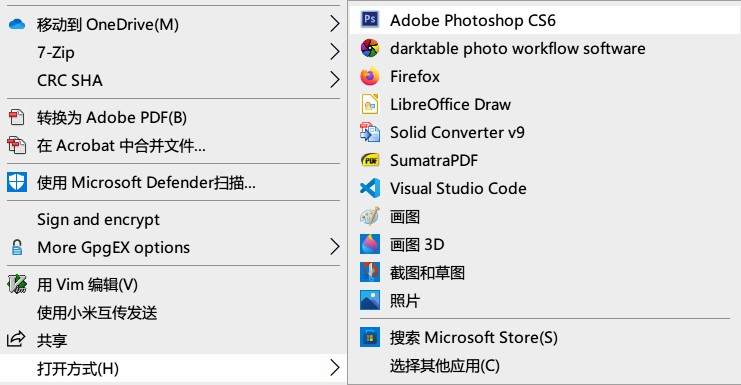
\includegraphics[width=9cm]{assets/Select_Open_with.jpg}
      \caption{更改打开方式}
      \label{Select_Open_with}
    \end{figure}
  \item 如果上一步找不到「Adobe Photoshop」,那么选择【打开方式】→【选择其他应用】。
    然后在弹出的对话框中寻找【Adobe Photoshop】,点击并选择【确定】。
    注意\regcolor{不要}勾选「始终使用此应用打开 \verb|.jpg| 文件」。
    \begin{figure}[htb!]
      \centering
      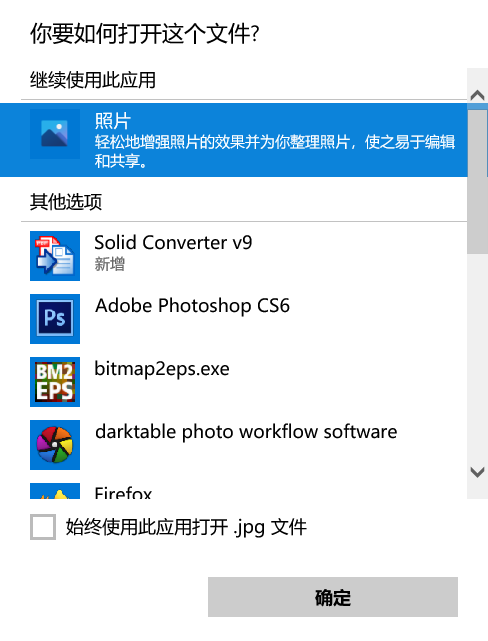
\includegraphics[width=5cm]{assets/Open_with.png}
      \caption{进一步选择}
      \label{Open_with}
    \end{figure}
  \item 如果上一步还找不到「Adobe Photoshop」,而你确实电脑上装有 Photoshop,那么可能需要手动找到 Photoshop 的那个可执行文件,也就是它的 \verb|exe| 文件。
    这个文件的路径——也就是软件的安装路径——在下一章我们会提到。
    一般来说是在 \verb|C:\Program Files| 或者 \verb|C:\Program Files (x86)| 之下的某个文件夹中。
\end{itemize}

\regcolor{如果你想永久地指派某一文件的打开方式,则可以在上面步骤的基础上,勾选【始终使用此应用打开 \texttt{xxx} 文件】。}
这样,系统内部的那张「表」就会被更改,系统以后都会用你指派的新应用来打开这种文件。

除了你手动更改之外,这张「表」还可能在这些情况被更改:

\begin{itemize}
  \item 系统安装更新,即 Windows Update 之后,这张表可能会被重置而丢失一些项目,造成某些文件突然无法打开。这往往是由于你使用的对应软件并不是原版,而是某种「精简版」所造成的。
  \item 新安装一个软件时,软件安装程序可能写入新的表项,来为即将安装的新软件的文件类型配置打开方式。
  \item Windows 的各种恶性 bug 和恶心操作。例如,Windows 会时不时用 Microsoft Edge 代替其他软件来打开网页文件和 \verb|pdf| 文件等。\CJKsout*{(微软你坏事做尽)}
\end{itemize}

如果你的文件关联某天突然失效,即某种类型的文件突然无法打开,但对应的软件工作正常,那么可以考虑是否是上面的原因。

\section{管理好你的文件}

管理好我们的文件,不外乎两个方面:

\begin{itemize}
  \item 对自己的文件进行整理归类。比起将所有文件「随手乱放」,如果我们将自己的文件按它们的性质、类别等归类存放,必然有助于提升我们的工作效率。
  \item 不把(重要)文件放在 C 盘。在前文我们说了,C 盘是 Windows 系统整个所在的地方。
    尽管发生这种情况的概率很低,但当我们的电脑因为这样或那样的原因损坏,而需要重装系统的时候,你会不得不失去 C 盘的所有文件——安装系统的第一步就是格式化 C 盘。
    让自己的文件远离 C 盘,是合理管理我们的文件的重要部分。
\end{itemize}

\subsection{为文件安家}

首先为你要放的文件选择一个合适的位置。

桌面,以及 Windows 系统预置的那些文件夹(「文档」「视频」「图片」等,打开【此电脑】就可以直接看到),除非按照后文所介绍的方法更改位置,否则全部是 C 盘内部的空间,因此在你手动更改它们的位置之前,\regcolor{不建议}将自己的文件放在这些地方。

另一方面,非 C 盘的分区,例如 D 盘甚至后续更多的磁盘分区,都是可以考虑的存放自己资料的位置。

找到一个合适的位置后,我们便可以建立一套自己的分类方法来对文件进行整理和分类。


\begin{itemize}
  \item 例如你有一些「学习资源」,你便可以在 D 盘或是什么别的盘建立一个名为「学习资源」的文件夹,再在其下——无论是按学科(例如「高数」「线代」「物理」),还是按时间(例如「大一上」「大一下」)——建立更多的子文件夹,来为它们进行更为详尽的分类。
  \item 再例如你有许多「大片」,你也可以按照地区、上映时间甚至是主演什么的为它们分类。
    不过鉴于大片不仅是名气大,占用空间也大,我们推荐腾出一个分区(甚至是一块硬盘)来存放它们。
\end{itemize}

总的来说,\regcolor{「为你的文件进行合理分类」}与\regcolor{「将你的硬盘进行合理分配」}便是这里的核心思想。

\subsection{定期打扫}

电脑里面的东西总是随着我们的日常使用而越积越多 \CJKsout*{(这里点名 QQ 的 \texttt{FileRecv} 和 \texttt{Image} 文件夹,藏得又深,又乱七八糟;还有微软的更新,一更一大堆)},所以定期检查你不需要的东西然后扔掉它们显得尤为重要。

对于系统分区 C 盘来说,你不去动它,它也会被塞入一些诸如系统临时文件、Windows 更新文件等等这些。
我们推荐新手用户们运用一些诸如「火绒安全软件」「360 电脑管家」之类的 app 中的清理功能进行文件的清理。

但是上述软件并不会把我们日常中积累的用户文件(例如你收到的课件、文档等)也清理掉,但在日常使用过程中,我们也会不可避免地产生许许多多的冗余文件,或是曾经需要而现在不再需要的文件。
这里不妨就来看看上文所讲的那个 \verb|FileRecv| 文件夹:

\begin{itemize}
  \item 这个文件夹默认位于 \verb|文档\Tencent Files\<QQ 号>\| 处,每个不同的 QQ 号都有一个属于自己的个人文件夹。
    如果你没有按照后文「更改用户文件夹的存储位置」迁移「文档」文件夹的话,这东西也在 C 盘里,因为「文档」是在 C 盘里的;
  \item 点开 \verb|FileRecv| ,你在使用 QQ 的过程中接收到的所有文件都在此处,其中通过手机发给电脑的文件存储于专属子文件夹 \verb|MobileFile| 中;
  \item 将 \verb|FileRecv| 文件夹中的所有文件检查一遍,有用的就如上文所述归类、无用的则直接删除,这就大功告成了。
\end{itemize}

事实上 QQ 为用户提供了更改用户个人文件夹位置的功能,但是似乎更改的时候并不会将你曾经接收的文件一并移走,着实不好用,这里并不推荐。

同样地,在你已经归好类的文件体系中,也要时不时进行检查,删去冗余与无用文件,这样能够保持你的文件系统简而精。
《礼记·大学》载:「苟日新,日日新,又日新。」如是而已。

\subsection{更改用户文件夹的存储位置 *}

上文提到了一个叫做 \verb|文档| 的文件夹,它是系统预置的一个用户文件夹。
在介绍这一部分之前,我们先简单提一下「用户文件夹」是什么。

\begin{figure}[htb!]
  \centering
  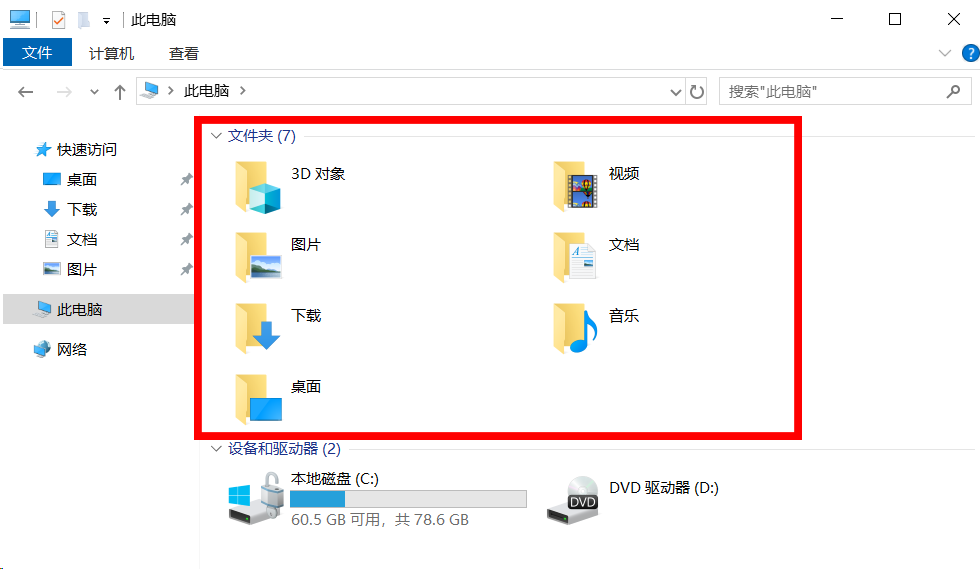
\includegraphics[width=11cm]{assets/User_directories.png}
  \caption{用户文件夹}
  \label{User_directories}
\end{figure}

如前所言,Windows 系统默认为用户准备了几个文件夹来进行文件的分类。
通过双击桌面上的【此电脑】,展开【文件夹】折叠项,这些文件夹就如图 \ref{User_directories} 所示。

Windows 系统的本意,是希望用户可以借助这些文件夹来辅助进行文件的整理。
可是,这些文件夹默认情况下全部位于 C 盘(路径是 \verb|C:\用户\<你的用户名>\| ),而把大量的个人文件放在 C 盘是我们所不建议的。
那这些系统「好心」准备给我们的文件夹就都不能使用了吗?
答案是否定的——通过迁移这些文件夹到 D 盘,我们可以在利用好这些用户文件夹的同时,保证自己的数据安全和系统稳定。

\begin{note}
  看到这几个文件夹中的「桌面」,你是否会有点奇怪?桌面为什么也是这里的一部分呢?
  事实上,桌面的本质也是一个用户文件夹。桌面上你放的文件、各个 app 的快捷方式都在这个文件夹中。
\end{note}

我们打开 \verb|C:\用户\<你的用户名>\| 可以看到全部的用户文件夹。
这些文件夹涵盖了「桌面」「文档」「图片」「音乐」「视频」等多种类别,并且都配有形象的图标,如图:

\begin{figure}[htb!]
  \centering
  
\includegraphics[width=4cm]{assets/All_User_Directories.jpg}
  \caption{更多用户文件夹}
  \label{All_User_Directories}
\end{figure}

我们的目的是把这些文件夹「迁移」到 D 盘(或者其他的某个磁盘,这里以 D 盘为例)。
这样,我们就可以充分地利用系统预置的这一批用户文件夹了。

右击某个我们想要迁移的文件夹(比如【桌面】),选择【属性】,然后切换到【位置】选项卡,如图:

\begin{figure}[htb!]
  \centering
  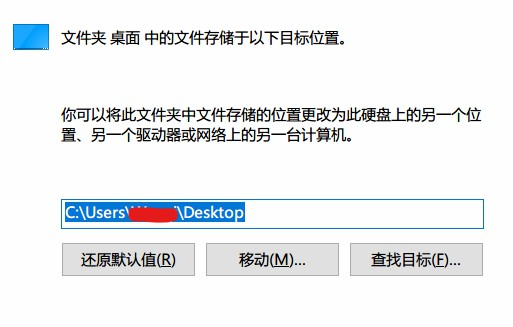
\includegraphics[width=8cm]{assets/Change_Directories.jpg}
  \caption{更改用户文件夹位置}
  \label{Change_Directories}
\end{figure}

我们将这里文本框中

\begin{verbatim}
  C:\Users\<你的用户名>\
\end{verbatim}

这一部分\regcolor{(注意:最后一个\texttt{Desktop}、\texttt{Documents}之类的名字不要动!)}\footnote{如果你不小心把一个用户文件夹的位置设置成了某个磁盘的根目录(比如说\texttt{D:\textbackslash}),会触发 Windows 系统的一个 bug,导致很难再改回来。\CJKsout*{(辣鸡 Windows)}}改成

\begin{verbatim}
  D:\
\end{verbatim}

\regcolor{也就是说,对于「桌面」而言,改完之后的完整路径是}

\begin{verbatim}
  D:\Desktop
\end{verbatim}

例如:

\begin{figure}[htb!]
  \centering
  \includegraphics[width=8cm]{assets/Destination.jpg}
  \caption{填入目标位置}
  \label{Destination}
\end{figure}

点击【应用】,提示「文件夹 ‘D:\textbackslash{}Desktop’ 不存在,是否新建该文件夹」,选择【是】。

紧接着提示「是否要将所有文件从原位置移动到新位置」,选择【是】。

一般来说移动操作很快就会完成。完成后,点击【确定】。
这样「桌面」文件夹就被成功地迁移到了 D 盘。
你可以打开 \verb|D:\桌面| 来查看其中的内容,与你桌面上真正看到的东西应该大同小异。

\begin{note}
  对于桌面而言,现在你放在桌面上的文件本质上就存在 D 盘里了。
  但我们依然不建议你在桌面上放太多文件——因为这样不方便你自己寻找。
\end{note}

\regcolor{强烈建议进行迁移的用户文件夹有:}\regcolor{「文档」「桌面」「下载」。}

\regcolor{建议进行迁移的用户文件夹有:}\regcolor{「视频」「图片」「音乐」。}

迁移完成之后,你可以在迁移之后的位置(比如 D 盘)看到这些文件夹。
它们现在不在原来的 \verb|C:\用户\<你的用户名>\| 那里了。

\begin{figure}[htb!]
  \centering
  \includegraphics[width=12cm]{assets/Moved_user_directories.jpg}
  \caption{新的用户文件夹位置}
  \label{Moved_user_directories}
\end{figure}

\practice

\begin{enumerate}
  \item 查看自己电脑的几个分区的「卷标」,并依照自己的文件分类习惯修改成自己所喜欢的名字。例如,叫「资料」或者「Files」就比「新加卷」或者没有卷标(会显示「本地磁盘」)要直观得多。
  \item 尝试把一个图片文件的扩展名改成 \verb|txt| ,然后用「记事本」打开它。你看到了什么?\textit{记得改回来哦!}
  \item 试着迁移用户文件夹到 D 盘或者其他非 C 盘的分区,然后利用这些用户文件夹帮助自己整理文件。\\
    注意迁移的时候千万看清楚目标路径是完整的 \verb|D:\Documents| 、 \verb|D:\Desktop| 这样的路径,而不是光秃秃的一个 \verb|D:\| 。
  \item 整理你的 QQ 文件接收文件夹 \verb|FileRecv| 。
  \item 选择你自己的几个文件和文件夹,把它们打包成一个压缩文件 \verb|MyArchive.zip| ,复制到其他的某个地方,尝试两种不同的解压方式「提取到当前位置」「提取到 MyArchive\textbackslash{}」。
  \item 创建一个文档(可以是纯文本文件 \verb|txt| 或者 Word 文档 \verb|docx| 等)并写入一些内容,然后制作它的两个快捷方式,并把这两个快捷方式放在两个与源文件都不一样的地方。试着双击打开那两个快捷方式,你发现了什么?删掉两个快捷方式中的一个,源文件被删除了吗?
    另一个快捷方式还在吗?
\end{enumerate}
\chapter{软件的寻找与安装}
\label{software-installation}

\begin{intro}
  软件的下载安装一直以来是困扰许多「电脑小白」的大问题——从哪里下?怎么下?下完怎么装?装完怎么办?什么,软件要收费?破解是什么?……这一章将对国内互联网环境下 Windows 软件的下载、安装和配置做一个简单的介绍。看完这一部分,你或许可以找到下面这些问题的答案,并慢慢对「怎么寻找软件」有一个初步的了解。
  \begin{itemize}
    \item 我想下载 xxx 软件,我应该去哪里找这软件?
    \item 网上全是病毒和垃圾软件,我应该怎么样最大程度保证自己电脑的安全?
    \item 为什么软件下到手还要安装?有的还要破解?为什么这么麻烦?
    \item 电脑里不是有个「Microsoft Store」吗?为什么那里面大多数软件都找不到?
  \end{itemize}
\end{intro}

直到今天,Windows 系统下依然没有一个广泛使用的集中化「应用商店」。与我们使用手机不同,在电脑上,我们若想安装某个软件,多数情况下需要到互联网上寻找软件的「安装包」,再自行将软件「安装」到电脑上来使用。

这部分,我们将具体介绍软件为什么要「安装」,如何从网上的万千垃圾软件中下载我们需要的软件,以及软件安装和配置的一些技巧和注意事项。

\section{安装与安装包}

在 Windows 系统上,应用是通过「安装包」来安装到系统上的。如果把 app 比作是一株植物,那安装包就是这棵植物生长之前的「种子」。我们要安装某个 app,就需要获取这个 app 的安装包,然后通过安装包将 app「安装」在电脑上。

为什么需要「安装包」而不直接分发应用本身呢?我们有必要稍微了解一下 app 在我们的电脑上「安装」的过程。

在\nameref{files-and-file-management}中我们看到,一款 app 除了主程序(一个 \verb|exe| 文件)外,还包含一大堆不可或缺的依赖文件和子文件夹,如图 \ref{ncm-files} 所示。

\begin{figure}[htb!]
  \centering
  \includegraphics[width=5cm]{assets/Netease_cloud_music_files.jpg}
  \caption{「网易云音乐」的目录结构}
  \label{ncm-files}
\end{figure}

安装包的作用之一,便是把上面这一大堆文件按照它们能够工作的结构「释放」到我们的电脑中的指定位置。而除了「释放 app 的文件」之外,安装包还会做一些其他事情,例如设置一些文件的打开方式(上一章中提到的那张「表」)、调整一些系统内部的参数等。可以说,软件安装的过程,不仅仅是将一大堆文件「释放」或者说「提取」到系统中的某一个位置的过程,它还会对系统进行或多或少的调教与更改。这就是「安装包」存在的意义——它帮助我们完成了这复杂的「安装」过程。

\section{如何上网寻找软件的安装包}

下面我们来探讨如何上网寻找我们需要的软件的安装包。

\subsection{优先考虑:官方网站}

当要获取一款 app 时,我们首先应该考虑的是 app 开发者的官方网站,即「官网」。比起在其他地方下载软件,从官网下载软件能最大限度地保证你所下载的东西是干净的。

然而,\regcolor{对于百度这样的搜索引擎,官网常常不是搜索结果中的第一个——百度搜索出来的前 3 条结果一般是广告}。例如,我们想要下载「WPS」,直接在百度中搜索「WPS 下载」,我们会得到图 \ref{baidu-wps-result} 那样的搜索结果。

\begin{figure}[htb!]
  \centering
  \includegraphics[width=10cm]{assets/Baidu_result.jpg}
  \caption{百度搜索「WPS 下载」的搜索结果}
  \label{baidu-wps-result}
\end{figure}

在图 \ref{baidu-wps-result} 中,我们搜索「WPS 下载」,然而在结果中:

\begin{itemize}
  \item {\color{Brown1} 第一条是「重庆天极网络有限公司」提供的广告。}
  \item {\color{Brown1} 第二条是「腾讯电脑管家」提供的广告,进去之后八成你会下载到「腾讯电脑管家」而不是「WPS」。}
  \item {\color{Brown1} 第三条是「马鞍山超聪网络科技」提供的广告。}
  \item {\color{Brown1} 第四条是「北京奥蓝德信息科技」提供的广告。}
\end{itemize}

\regcolor{上面这四条全部是广告}。这意味着进入这些页面,你八成下载不到干净的「WPS」,而只能下载到一堆垃圾。

\begin{itemize}
  \item {\color{Chartreuse3} 第五条是 WPS 官网。注意看它的网址是 \texttt{www.wps.cn},这是 WPS 的官方网站。}
  \item {\color{Chartreuse3} 第六条也是官网。}
  \item {\color{Brown1} 第七条又是「腾讯电脑管家」的广告。}
  \item {\color{DarkGoldenrod2} 第八条是第三方下载站「华军软件园」的链接。我们在后面会提到,当官网不可用的时候,怎么从这种第三方下载站下载软件。}
\end{itemize}

鉴别一个网站到底是不是官网,我们主要可以观察这么几个地方:

\begin{itemize}
  \item 看网址。一般官网的网址都是企业或者软件的名字。例如:
  \begin{itemize}
    \item WPS 的官网是 \verb|www.wps.cn|。
    \item QQ 的官网是 \verb|im.qq.com|。微信的则是 \verb|weixin.qq.com|。(腾讯首页:\verb|qq.com|)
    \item 网易云音乐的官网是 \verb|music.163.com|。(网易官网:\verb|163.com|)
    \item ……
  \end{itemize}
  \item 排除法。没有哪个软件厂商的名字是叫做「xx 软件站」「xx 下载站」「xx 软件园」的。带有这些名字的全部是第三方下载站。
  \item 语义判断。一般广告网站的标题都与搜索关键词没有任何实质上的联系。我们不妨再看上面的搜索结果中的前四条广告:
  \begin{itemize}
    \item 第一条:「办公软件下载客户端 2021 年正版免费下载」,只字不提「WPS」或者「金山办公」。(WPS 是金山公司开发的办公软件)
    \item 第二条:「wsp 办公软件下载-2021 官方版-电脑管家软件中心」,挂羊头卖狗肉而且挂错了。
    \item 第三条、第四条类似第一条。
  \end{itemize}
\end{itemize}

进入软件的官方网站之后,我们搜索「全部产品」「软件下载」之类的选项,就可以找到我们所需要的软件的安装包。例如从 WPS 的官网上下载 WPS 软件:

\begin{figure}[htb!]
  \centering
  \includegraphics[width=10cm]{assets/Download_WPS.jpg}
  \caption{从官网下载 WPS}
  \label{download-wps}
\end{figure}

\subsection{直面深渊:第三方软件站}

在某些时候,我们确实找不到一个软件的官网,或者因为这样那样的原因不能去官网下载某个软件。这时,我们将不得不直面深渊,进入「xx 软件园」「xx 软件站」「xx 下载站」这样的网站下载软件。

这种网站一般是可以下载到我们想要的东西的——前提是,你足够小心,不点到那些所谓「高速下载器」「P2P 下载器」的虚假链接。下面我们会手把手实操这个过程。

假设我们要下载「SecureCRT」这款软件。我们在百度上搜索「SecureCRT 下载」,并主动避开那些明显骗人的广告,点击了这个看似还能接受的「华军软件园」网站:

\begin{figure}[H]
  \centering
  \includegraphics[width=8cm]{assets/Huajun_1.jpg}
  \caption{「华军软件园」上的「SecureCRT」}
  \label{huajun-1}
\end{figure}

重点来了:\regcolor{进入这个网站,请主动避开所有「高速下载」「极速下载」「P2P 极速下载」这样的按钮,选择「普通下载」「本地下载」这样的按钮}:

\begin{figure}[H]
  \centering
  \includegraphics[width=10cm]{assets/Huajun_2.jpg}
  \caption{不要选择【高速下载】,选择【本地下载】}
  \label{huajun-2}
\end{figure}

点击之后我们会跳转到这样一个「下载地址」的页面。同样地,我们\regcolor{不要点击「需优先下载高速下载器」之下的所有连接,而要点击「普通下载地址」下方的「通用网络下载」或者「电信网络下载」}:

\begin{figure}[H]
  \centering
  \includegraphics[width=8cm]{assets/Huajun_3.jpg}
  \caption{不要点击「需优先下载高速下载器」之下的所有链接,选择「普通下载地址」下方的链接}
  \label{huajun-3}
\end{figure}

使用下方两个链接下载到的文件如图 \ref{real-securecrt},体积约 50 MB,符合这个软件的体量;它是一个压缩包,一般解压缩之后就能得到软件的安装包。而使用上方所谓「高速下载」下载到的文件是 \ref{fake-securecrt},体积只有 1 MB,而且是一个不明的「可执行文件」(exe 文件),这是不正常的。在本章的最后,我们会使用一台虚拟机来演示这「高速下载器」会干什么。

\begin{figure}[htb!]
  \centering
  \begin{minipage}{6cm}
    \centering
    \includegraphics[width=5cm]{assets/Real_SecureCRT.png}
    \caption{点击「普通下载」得到的真正的软件安装包}
    \label{real-securecrt}
  \end{minipage}
  \qquad
  \begin{minipage}{6cm}
    \centering
    \includegraphics[width=5cm]{assets/Fake_SecureCRT.png}
    \caption{点击「高速下载」得到的假的软件安装包}
    \label{fake-securecrt}
  \end{minipage} 
\end{figure}

\subsection{另辟蹊径:软件公众号及其他小众渠道}

另一种「另辟蹊径」的方法,是通过一些「小众渠道」,例如一些分享软件的微信公众号来下载软件。这不失为一种好方法——那些人们口口相传的优质公众号一般会把常用软件的「干净」安装包分门别类地整理分享,与「xx 下载站」相比,免去了「高速下载器」的烦恼。

但是,这种公众号一般软件不是特别多——你总有一天没法从它们那里找到想要的软件。此外,这些公众号一般使用百度网盘来分享文件,而众所周知百度网盘是对非会员限速的,这必然对使用体验有一定影响。不过总的来说,这依然是一种值得推荐的方法。

\begin{note}
  对于这类公众号,我们并没有做太多的收集,因此无法在此推荐。大家可以在 B 站、贴吧、微博等地方自行寻路。
\end{note}

\subsection{他山之石:第三方的「软件管家」}

除了手动在网上——无论是在官网,从第三方下载站,还是从那些整理网站的公众号上——下载软件的安装包之外,有一些第三方的「软件管家」也能帮助我们找到所需要的软件。这些软件管家有的是电脑厂商所维护的,例如「联想软件管家」「华为软件管家」;有的是一些公司所维护的,比如「360 软件管家」「腾讯软件管家」等(名字不一定是这样,可以类比)。

一般来说,那些由电脑厂商所维护的「软件管家」,往往相对干净、不带「全家桶」式的捆绑;而那些第三方企业维护的「软件管家」,一般都会或多或少地提示用户安装它们的「全家桶」。比如,如果你使用「360 软件管家」,那它一定会用某些手段提示用户去安装「360 安全卫士」以及一系列其他软件。因此,你可以根据自身机器的实际情况,按需选择这样的「软件管家」类 app。

\section{安装软件}

假设经过与流氓网站的「斗智斗勇」,你成功地下载到了某款软件的安装包。取决于软件,你下载到的可能是下面三种文件中的某一种:

\begin{itemize}
  \item 一个光秃秃的 \verb|exe| 文件。
  \item 一个压缩包,例如 \verb|zip| 或 \verb|rar| 文件。
  \item 一个扩展名是 \verb|iso| 的文件。
\end{itemize}

对于第一种情况,我们直接双击这个 \verb|exe| 文件就能启动安装进程。对于第二种情况,我们需要解压缩这个压缩包到某处,然后在解压出来的文件中找到名字类似「\verb|setup.exe|」或「\verb|install.exe|」的程序双击打开。对于第三种情况,我们右击这个 \verb|iso| 文件,选择【打开方式】→【文件资源管理器】,然后在弹出的新窗口中找到名字类似「\verb|setup.exe|」或「\verb|install.exe|」的程序双击打开\footnote{当你这样打开 \texttt{iso} 文件后,这个文件会临时被「映射」成电脑里的一个新「分区」,打开【此电脑】就能发现它。在你安装完成后,可以打开【此电脑】,右键这个分区选择【弹出】来让这个分区消失。}。

启动安装器后,我们一般按提示【下一步】操作即可完成安装。

\begin{note}
  此过程中也要留心!跨过了「高速下载器」的坎,可不要又掉进了捆绑软件的坑。有一些软件在安装程序中也会像「高速下载器」一样勾选了一些捆绑软件、浏览器主页劫持什么的,这些选项可能出现在安装过程中的任何阶段,一定要注意取消勾选再进行下一步。
\end{note}

在安装过程中需要特别注意的一件事,便是「软件安装位置」,即安装包把软件自身的各种文件「释放」的位置。

在上一章中我们提到过,不要把大量的软件安装在 C 盘——安装到 D 盘或其他磁盘分区是更好的选择。一般来说,软件默认会把自己「释放」在以下两个路径之一:

\begin{verbatim}
  C:\Program Files\<厂商名字>\<软件名字>\
  C:\Program Files (x86)\<厂商名字>\<软件名字>\
\end{verbatim}

在上一章中我们提到了「快捷方式」,在你的电脑桌面上就有许多软件可执行文件的快捷方式。右键它们选择【属性】,你就能看到这些已经安装的软件的位置。看看它们中的一些是不是在 \verb|C:\Program Files\| 或者 \verb|C:\Program Files (x86)\| 下?

\verb|Program Files| 和 \verb|Program Files (x86)| 这两个文件夹,即系统预置的两个用来安装 app 的文件夹,都位于 C 盘根目录下。然而,我们希望把软件安装到 D 盘。这里推荐一个简单好用的方法:直接将默认路径中的 \verb|C:| 改成 \verb|D:|。例如:

\begin{verbatim}
  D:\Program Files (x86)\Tencent\QQ\
\end{verbatim}

这就是在 D 盘安装 QQ 软件的一个很合适的路径。这样做能保持一个比较干净的目录结构。你的 D 盘下会因此多出 \verb|Program Files| 和 \verb|Program Files (x86)| 这样的两个文件夹,用来专门在 D 盘安装软件。

\begin{figure}[htb!]
  \centering
  \includegraphics[width=8cm]{assets/Change_C_to_D.jpg}
  \caption{一般把这个 \texttt{C:} 改成 \texttt{D:} ,就能得到一个不错的 D 盘安装软件的路径}
  \label{change-c-to-d}
\end{figure}

如图 \ref{sogou-install} 所示,有一些软件的安装包不是「下一步」型的,而只有一个「立即安装」的按钮。一般这种情况,可以展开「自定义安装」之类的选项,然后更改软件的安装位置。

\begin{figure}[htb!]
  \centering
  \includegraphics[width=8cm]{assets/Sogou_change_directory.jpg}
  \caption{对于只有一个「立即安装」按钮的安装包,一般找到「自定义安装」的选项展开后即可更改安装位置}
  \label{sogou-install}
\end{figure}

\section{软件收费、破解和自由软件}

很多软件是需要购买的,包括 Windows 系统本身(一般你购买电脑时,电脑厂商已经帮你出了买 Windows 这部分钱)。常见的专业软件,从平面设计领域的 Adobe 家族的 Photoshop、Premiere Pro,工程领域的 Autodesk 家族的 AutoCAD、3ds MAX,到开发领域的 JetBrains 家族的 IDEA、PyCharm,甚至于我们每天都在用的 Word 和 PowerPoint,这些软件全部都需要付费购买。图 \ref{buy-adobe} 是购买正版 Photoshop(俗称的 PS)软件的页面——定价 888 元一年。

\begin{figure}[htb!]
  \centering
  \includegraphics[width=6cm]{assets/Adobe.jpg}
  \caption{Adobe 的「Creative Cloud 中国摄影计划」套装,包含 Photoshop 和 Lightroom Classic 两款软件,定价 888 元一年。}
  \label{buy-adobe}
\end{figure}

而由于这样或那样的原因,我们在实际生活中,或多或少都在「没有付费而白嫖这些软件」。这是因为我们使用的这些软件被「破解」了。破解之后,软件的计费功能失效,原本收费的软件通过某种方式变成了可以免费永久使用的软件。大体上,网上流传的破解软件一般有这么两种形式:

\begin{itemize}
  \item 一种是已经完全破解了的收费软件。这种软件已经经过修改,安装包往往也是民间自行制作的,可以直接走正常流程安装,安装后打开就可以无限制地使用。例如一些 Adobe 软件破解版套装。
  \item 另一种是使用收费软件的试用版本安装软件,再外加「破解补丁」。这种软件的安装包依然是使用官方原版的安装包,安装完成之后,通过某种「打补丁」的方式来外挂「欺骗」这官方原版的软件,让原版软件以为用户已经购买,从而解锁全部的功能并让用户无限制使用。常见的 Office 软件的破解、Autodesk 软件的破解都属于此类。
\end{itemize}

使用破解软件终究是一件「上不得台面」的事情。一般来说,如果你使用破解软件作为私下的个人使用、学习,软件厂商大多是不会进行追究的。但是,如果你将破解软件(或者说,盗版软件)用于商业用途,那必然迟早会受到追究。尽管实际生活中软件厂商维权的积极程度各有差异,尽管大家会因为各种各样的原因不得不去使用盗版和破解,但我们仍然呼吁大家支持正版软件,万不得已使用盗版、破解软件时,仅作为非商业的个人和学习用途。

与那些用来盈利的商业软件不同,「自由软件」(free software)不仅是「免费」(Free as in `free beer')的,而且是「自由」(Free as in `free speech')的。对于自由软件,人们不仅可以无偿使用,还能自由地复制、分发,甚至是在一定条款之下修改它们。自由软件的原始代码是公开的,下载使用是免费的,开发者是多元包容的。近些年来,自由软件作为一种新浪潮在互联网上的发展不断壮大,自由软件在越来越多的领域开始出现。

在今天,一些自由软件已经开始动摇过去一些不可或缺的商业软件的地位。我们鼓励大家在实际使用电脑的过程中,多多尝试、使用一些优质自由软件。在《Missing》的后续章节中,我们会推荐一批各个领域的优质软件,其中就有许多自由软件的身影。

\section{UWP 应用和 Microsoft Store *}

作为 Windows 亲爹的微软早在数年前就意识到,Windows 系统下一直缺少一个官方维护的、像 Apple 的 App Store 那样的「集中化」的软件中心,用户下载软件只能像上文那样上网去苦苦找寻。彼时的微软公司正打算进军手机行业,想要和安卓与 iOS 形成「三足鼎立」之势,微软于是心想:不如弄一种新的 app 格式,这种新的 app 不仅能在我们的 Windows 电脑上运行,还可以在手机上运行;然后我们再顺带弄一个全是这种新格式 app 的应用商店,可谓一举两得。于是微软就这么干了:这种新的 app 格式叫做「通用 Windows 平台应用」(Universal Windows Platform,简称「UWP 应用」),这个应用商店就是我们电脑里的「Microsoft Store」:

\begin{figure}[H]
  \centering
  \includegraphics[width=5cm]{assets/MS_Store_1.jpg}
  \caption{Windows 10 中的 Microsoft Store}
  \label{ms-store-in-windows-10}
\end{figure}

可是,时过境迁:微软终究没有能在手机市场打下一片江山,微软做的手机系统最终在近两年宣布「谢幕」。可是微软心想,这「UWP 应用」的先进构想和 Microsoft Store 不能开了头就没了尾,因此它们直到今天依然被保留在 Windows 系统之中。

如果你有打开过「Microsoft Store」,如图 \ref{ms-store},你会发现,其中有一些应用是我们日常生活中的常用应用,而另外的大多数应用,我们都从来没有听说过。而事实上,如果你去仔细查看那里面的常用应用,会发现它们往往更新得没有官网勤快,有些甚至已经停止了更新。

\begin{figure}[htb!]
  \centering
  \includegraphics[width=10cm]{assets/MS_Store_2.jpg}
  \caption{Microsoft Store 的界面}
  \label{ms-store}
\end{figure}

事实上,这就是 Microsoft Store 的现状:作为推广「UWP 应用」的第一线,它没有什么很拿得出手的「杀手锏」;作为一个「xxx 软件中心」的替代品,它的应用相当不全。微软在 Microsoft Store 和 UWP 应用上充满了雄心壮志,却最终落得今天的结局。

\section{演示:「高速下载器」到底会干什么}

\begin{warning}
  \textbf{请不要在自己电脑上尝试打开这种「高速下载器」!}
\end{warning}

在上文中我们演示下载「SecureCRT」时,如果点选了「高速下载」,会得到如图 \ref{gao-su-downloader-1} 的一个只有 1 MB 的可执行文件:

\begin{figure}[H]
  \centering
  \includegraphics[width=5cm]{assets/Gao_su_1.jpg}
  \caption{下载到的「高速下载器」,一般来说体积在 1 MB 左右}
  \label{gao-su-downloader-1}
\end{figure}

双击这个「高速下载器」,弹出的窗口如图 \ref{gao-su-downloader-2}。可以看到,右方有四个捆绑软件的复选框被默认勾选:「360 安全浏览器」「QQ 游戏大厅」「U 号租」「百度网盘」,右下方还有一个「六间房直播」。假设我们足够理智,取消勾选了这里的所有的勾,然后点击「快速安装」。等待进度条跑完之后,则会来到图 \ref{gao-su-downloader-3} 的界面。这个界面上又有两个软件捆绑「绝地求生」和「傲视霸主」,以及一个「使用 360 安全导航」的复选框。

\begin{figure}[htb!]
  \centering
  \begin{minipage}{6cm}
    \centering
    \includegraphics[width=5cm]{assets/Gao_su_2.jpg}
    \caption{「高速下载器」打开后的界面}
    \label{gao-su-downloader-2}
  \end{minipage}
  \qquad
  \begin{minipage}{6cm}
    \centering
    \includegraphics[width=5cm]{assets/Gao_su_3.jpg}
    \caption{「高速下载器」完成下载后的界面}
    \label{gao-su-downloader-3}
  \end{minipage} 
\end{figure}

全部取消这些复选框,我们点击「打开文件」,终于打开了我们想要的 SecureCRT 的安装包——一个名为 \verb|SecureCRT.rar| 的,体积约 50 MB 的压缩包。而这就是我们直接点选「普通下载」直接就能下载到的东西。

如果我们没有取消上面的这些勾选,那会是什么结局呢?

\begin{warning}
  请勿模仿!
\end{warning}

\begin{figure}[H]
  \centering
  \begin{minipage}{8cm}
    \centering
    \includegraphics[width=7cm]{assets/Gao_su_4.jpg}
    \caption{被乱七八糟的软件「占领」的电脑桌面}
    \label{gao-su-downloader-4}
  \end{minipage}
  \qquad
  \begin{minipage}{4cm}
    \centering
    \includegraphics[width=3cm]{assets/Gao_su_5.jpg}
    \caption{充满各种乱七八糟的软件的「开始」菜单}
    \label{gao-su-downloader-5}
  \end{minipage} 
\end{figure}

我们得到的结论是:

所谓「高速下载器」最后下载到的就是你点击「普通下载」得到的东西,纯属脱裤子放屁。

而「高速下载器」在整个过程中带有许多的捆绑勾选,一旦不留神你的电脑就会被各种垃圾软件充斥。

\begin{note}
  这种流氓的「高速下载器」一般被戏称为「高速下崽器」。
\end{note}

\practice

\begin{enumerate}
  \item 在图 \ref{how-to-download-it-1} 至图 \ref{how-to-download-it-3} 中,怎样操作最不可能下载到垃圾?
  \begin{figure}[htb!]
    \centering
    \begin{minipage}{8cm}
      \centering
      \includegraphics[width=7cm]{assets/How_to_1.jpg}
      \caption{下载软件「谷歌浏览器」}
      \label{how-to-download-it-1}
    \end{minipage}
    \qquad
    \begin{minipage}{4cm}
      \centering
      \includegraphics[width=3cm]{assets/How_to_2.jpg}
      \caption{下载软件「QQ」}
      \label{how-to-download-it-2}
    \end{minipage}    
    \\
    \vspace{1ex}
    \begin{minipage}{12cm}
      \centering
      \includegraphics[width=10cm]{assets/How_to_3.jpg}
      \caption{下载软件「WPS」}
      \label{how-to-download-it-3}
    \end{minipage}
  \end{figure}
  \item 图 \ref{how-to-download-it-4} 的界面中有几个捆绑勾选?
  \begin{figure}[htbp]
    \centering
    \includegraphics[width=8cm]{assets/How_to_4.jpg}
    \caption{下载「微信电脑版」时不慎下载到的「高速下载器」}
    \label{how-to-download-it-4}
  \end{figure}
  \item 下载「微信电脑版」,下面三个文件体积中哪一个最可能不是垃圾软件?
  \begin{enumerate}
    \item 640 KB 
    \item 1.1 MB
    \item 150 MB  
  \end{enumerate}
  \item 下面四个软件安装路径,谁最合适?其他的不合适在哪里?
  \begin{enumerate}
    \item 安装 Steam:\verb|C:\Program Files\steam|
    \item 安装微信电脑版:\verb|D:\Program Files (x86)\Tencent\Wechat|
    \item 安装 Vivado:\verb|D:\软件\Xilinx\Vivado|
    \item 安装网易云音乐:\verb|桌面\我的软件\Cloudmusic|
  \end{enumerate}
  \item 假设某个软件已经被安装在了一个地方,我现在想把这个软件放到另一个地方,可以直接剪切移动整个软件的目录到另一个地方吗?
  \item 查看自己电脑上 5 个不同软件的安装位置,并打开它们的安装目录,看一看里面的结构。
\end{enumerate}
\chapter{基本维护和安全防护}
\label{cha:basic-maintenance}

\begin{intro}
  上一章我们认识到了「网络世界的险恶」——恶意软件层出不穷、安装捆绑无处不在。在这样的环境之下,掌握电脑的简单维护方法、学习如何保护自己的安全,就显得尤为重要了。阅读完这章的内容,你将找到下面这些问题的答案:
  \begin{itemize}
    \item 不小心安装了不想要的软件,怎么卸载它们?
    \item 为什么打开有些软件时,系统总是提示「是否运行此应用对你的电脑进行更改」?
    \item 杀毒软件?安全中心?电脑管家?到底用什么?
    \item 为什么电脑天天都在「更新」?
    \item 网络上不干净的东西这么多,我要怎么才能「洁身自好」?
  \end{itemize}
\end{intro}

掌握一定的电脑维护的方法,例如软件的卸载、恶意软件的排查,以及了解一些电脑的安全维护的策略和措施,是保障我们「网上冲浪」安全的重要一环。在这一章,我们将了解一些常用的电脑维护技巧,以及一些电脑安全方面的常识。

\section{软件的卸载}

上一章我们介绍了软件的寻找与安装,这里我们就来介绍软件的卸载。软件的安装需要通过安装包来进行,而软件的卸载则是安装的逆过程,除了删除软件自身的文件之外,还会撤销一些写入系统的修改,解除一些文件关联等。因此,软件的卸载也需要通过软件自身提供的卸载工具进行,不是找到安装目录把所有文件全部删除了事,更不是直接删除桌面上的图标(快捷方式)。

在 Windows 11 系统上,一般的软件卸载可以按下面的步骤进行:

\begin{itemize}
  \item 打开系统设置。
  \item 在界面左侧点击【应用】,然后在右侧选择【安装的应用】(部分版本称【应用和功能】),如\autoref{fig:Applications_11}。
  \item 等待右侧下方的列表加载完成。这个列表就是你的电脑上安装的所有软件。找到你不想要的软件,点击这一行右侧的【\makebox[.8em]{⁝}】,再点击【卸载】,如\autoref{fig:Uninstall_an_app_11}。
    \begin{figure}[htb!]
      \centering
      \begin{minipage}{.49\textwidth}
        \centering
        \includegraphics[width=\textwidth]{assets/basic/Applications_11.png}
        \caption{打开 Windows 11 中的应用列表}
        \label{fig:Applications_11}
      \end{minipage}
        \begin{minipage}{.49\textwidth}
        \centering
        \includegraphics[width=\textwidth]{assets/basic/Uninstall_an_app_11.png}
        \caption{在 Windows 11 中卸载应用}
        \label{fig:Uninstall_an_app_11}
    \end{minipage}
    \end{figure}
  \item 之后根据提示卸载即可。
\end{itemize}

而在 Windows 10 上则是这样:

\begin{itemize}
  \item 打开系统设置。
  \item 选择【应用】,如\autoref{fig:Applications_10}。
  \item 稍等片刻以使得列表完全加载。在这个界面上,会列出电脑中安装的所有软件。找到我们不想要的软件,然后点击两次【卸载】,如\autoref{fig:Uninstalling_an_app_10}。
  \begin{figure}[htb!]
    \centering
    \begin{minipage}{.44\textwidth}
      \centering
      \includegraphics[width=.8\textwidth]{assets/basic/Applications_10.png}
      \caption{打开 Windows 10 中的应用列表}
      \label{fig:Applications_10}
    \end{minipage}
    \begin{minipage}{.55\textwidth}
      \centering
      \includegraphics[width=.9\textwidth]{assets/basic/Uninstalling_an_app_10.png}
      \caption{在 Windows 10 中卸载应用}
      \label{fig:Uninstalling_an_app_10}
    \end{minipage}
  \end{figure}
  \item 根据提示进行卸载操作即可。
\end{itemize}

一般来说,卸载很快就能完成。但需要特别注意的是,一些软件的卸载界面错综复杂,\regcolor{充斥有大量的无关选项}(例如【再想想】【我要重装】),因此在点选时务必十分小心。\regcolor{甚至有些软件在卸载完成后会诱导用户装一个新的其他软件,请千万注意。}例如:

\begin{figure}[htb!]
  \centering
  \includegraphics[width=.6\textwidth]{assets/basic/WDP_software_manager.pdf}
  \caption{诱导安装}
  \label{Confusing_Uninstall}
\end{figure}

有的软件可能会在卸载完成后,提示你需要重启电脑来进行一些最后的清理工作。通常,我们可以选择立即重启;如果你手头还正需要使用电脑,也可以在合适的时候手动重启。

\section{应用的权限与 UAC 弹窗}

这一节我们简单介绍 Windows 系统中的权限机制\footnote{如果你在使用中压根没见过\autoref{fig:UAC_popup} 这样的窗口(即 UAC 弹窗),那么这一节的内容对你可能不适用。你可以去\chapref{cha:user-and-ms-account}一章了解更多信息。}。在 Windows 系统中,一个程序在一开始启动时仅被赋予了有限的权限——它不能更改系统的一些关键设置,不能在系统中安装新的软件,不可以动一些关键数据。对于大多数程序来说,这些权限就够用了:一般的程序也不会去动那些系统级的设置或者给你装一个什么新软件。它们只需要安分守己地读写自己的文件,帮助用户完成工作就可以了。

但是,在一些特殊的情况下,这种有限的权限对程序来说会变得不够用。例如:

\begin{itemize}
  \item 对于\regcolor{安装包}来说,安装包本身的工作就是安装新的软件,而有限的权限禁止了这种行为。
  \item 对于一些\regcolor{专业软件}来说,它需要连接到一些系统级的部件才能工作,而有限的权限禁止了这种行为。
  \item 对于一些\regcolor{「系统优化」类的软件}来说,它本身就是需要更改系统设置的,而有限的权限禁止了这种行为。
\end{itemize}

\begin{wrapfigure}[12]{r}{6.5cm}
  \centering
  % \vspace*{-.5cm}
  \includegraphics[width=6cm]{assets/basic/UAC_popup.png}
  \caption{一个 UAC 弹窗}
  \label{fig:UAC_popup}
\end{wrapfigure}

此时,程序需要提升自己的权限来完成自己的工作,这个过程称为「提权」。而右图展示的这种弹窗(「你要允许此应用对你的设备进行更改吗」,称为「UAC 弹窗」),则是程序在向系统申请提权时,系统对用户的提示。这样就能解释,为什么在大多数安装或者卸载软件的时候,系统都会弹出这个窗口询问我们;而只有我们点击【是】,安装或者卸载才能正常继续了。

那么这种 UAC 弹窗的意义是什么呢?想象一下这个场景:你电脑上的某个垃圾软件留下的「种子」正在蠢蠢欲动,想要给你电脑安装一套恶意软件。然而,默认情况下,这枚「种子」没有足够的权限,因此它邪恶的计划就这样直接被粉碎了——没有提升的权限,它就没有办法进行软件安装。这也告诉了我们一个重要的事实:\regcolor{如果电脑弹出了不明的 UAC 弹窗,请一律拒绝}

一般来说,「提权」这件事是软件自行向系统申请的。但是有一些软件设计时考虑不周全,它不会自行向系统申请提权,但它正常工作又必须有提升的权限。对于这样的软件,我们可以在启动它时点击右键,选择【以管理员身份运行】,在 UAC 弹窗中选择【是】,就可以手动赋予这个软件提升的权限了。或许你会在使用中发现,一些老旧的软件在安装时就常常需要这么做。

当然,这一套权限系统是有很多空子的。提升的权限具有从属关系——如果某个程序被提权,那么由它打开的其他程序也默认具有特权。因而,如果你为一个不怀好意的程序赋予了特权,那它就可以为所欲为了,因为它能够不动声色地给其他程序特权,然后做一些不好的事情。所以,最终我们还是需要控制住自己电脑上软件的来源,不要让「不干净」的软件来到我们的电脑上。因此,\regcolor{不运行来源不明的可执行文件},是保证安全的根本。

\section{合理使用杀毒软件和安全软件}

合理使用各种杀毒软件、安全软件(后文统称「安全软件」)可以保护你的电脑安全,然而若运用得不合理,也会极大影响我们使用电脑的体验。今天,市面上有大量优秀的国内外安全软件供我们选择——例如,国产的「360 安全卫士」「火绒安全软件」「瑞星杀毒软件」,以及国外的「卡巴斯基」「诺顿」等。同时,Windows 操作系统亦内置了一款「Windows 安全中心」(旧称「Windows Defender」),它也提供了强大的病毒防护和安全保护等功能,如下图所示。这里,我们不具体地推荐某一款安全软件,而是会向你介绍一些相对合理地使用这类软件的方法。

\begin{figure}[htb!]
  \centering
  \includegraphics[width=.64\textwidth]{assets/basic/Windows_Security.png}
  \caption{Windows 安全中心}
  \label{fig:Windows_Security}
\end{figure}

首先,\regcolor{永远不要在电脑上同时安装多于一个杀毒软件}。例如,安装了「360 安全卫士」或者「360 杀毒」,就不要再安装「火绒安全软件」或者「腾讯电脑管家」。如果你同时安装多个安全软件,不仅没有必要,它们之间还会因权限冲突而互相「攻击」\CJKsout*{(这就是养蛊)}。

\regcolor{当心「全家桶」。}大型软件厂商都会希望用户能选择自己的整套产品系列。以「腾讯电脑管家」为例,它会以各种方式推荐用户安装包括但不限于「QQ 浏览器」「QQ 游戏」「腾讯桌面整理」等一整套腾讯产品。但事实上,很多时候,我们只是希望安装一款安全软件或杀毒软件来保护我们的电脑罢了。稍不留神,这些软件就会因为某个隐秘的角落的勾勾没有去掉,而来到我们的电脑上。

\begin{figure}[htb!]
  \centering
  \includegraphics[width=.64\textwidth]{assets/basic/Disable_360_ads.png}
  \caption{360 安全卫士的一些设置项}
  \label{fig:Disable_360_ads}
\end{figure}

我们安装安全软件是为了保障电脑安全,而不是希望这些软件来拖慢我们电脑的运行速度。因此,它们需要经受一些「调教」,才能更好地为我们服务。具体地说,我们可以\regcolor{关闭那些无用的功能和提示},例如每次开机时的启动时间提示、桌面上碍事的「一键加速」加速球、各种「资讯」弹窗广告和「猜你喜欢」搜索框等。这些东西与安全毫不相关,反而有些喧宾夺主。将它们关闭,可以让我们的电脑更加清爽,也不会影响到安全软件的正常工作。以「360 安全卫士」为例,我们可以在软件设置的【开机小助手】【推广设置】【广告资讯设置】等页面中,关闭我们不需要的功能,如\autoref{fig:Disable_360_ads} 所示。

\section{Windows 更新——让人又爱又恨的「更新」}

Windows 一直在不断的更新之中——这里的「更新」指的不是诸如「Windows 7」「Windows 10」这样的大版本的更新,而是那时不时阻碍我们关机睡觉的「Windows 更新」。打开系统设置,Windows 10 选择【更新与安全】(下左图)、Windows 11 选择【Windows 更新】(下右图),你就能看到现在可用的一些 Windows 更新以及它们的状态。

\begin{figure}[htb!]
  \centering
  \includegraphics[width=.85\textwidth]{assets/basic/Update.png}
  \caption{Windows 10 (左)与 Windows 11(右)的「Windows 更新」界面}
  \label{Windows_Update}
\end{figure}

在今天的 Windows 系统中,Windows 更新主要会包括以下这些内容:

\begin{itemize}
  \item Windows 系统本身的补丁。其中包括一些对系统高危安全漏洞的「修补」,是微软给 Windows 中存在的安全问题的补丁。
  \item 电脑驱动程序的更新。这保证了你电脑上运行的驱动程序是最新的,(理论上)能更好地发挥电脑的性能。
  \item 电脑的「体验更新」。这是一些最直观的更新,主要包括系统外观与体验的优化。相比上面两项,这些更新更加容易被我们感知。
\end{itemize}

这样看来,Windows 更新应该是一件人见人爱的美事,但事实并非如此。除了阻碍我们关机睡觉之外,Windows 更新还存在一定风险——那些第一晚跑 Windows 更新,然后第二早电脑就无法启动的「翻车」事件已是屡见不鲜。事实上,Windows 更新和我们手机的「系统更新」本质一样,都会触碰系统最核心的部分。如果这个过程中出了一些差错,就可能让系统损坏,轻则功能不正常,重则完全无法启动。

但我们不至于因噎废食,而且还是基本上噎不着的情况下。事实上,那些因为 Windows 更新导致系统损坏的情况,大都是因为用户在电脑更新时手动打断,而非 Windows 更新自身的问题。Windows 更新提供了大量的系统安全补丁和更新,它们对保护系统安全的意义相当重大。所以,仅仅为了可能因不当操作损坏电脑就禁用 Windows 更新并不是理智的做法,况且,现在完全关闭 Windows 更新的步骤也挺复杂。

因此,我们所需要做的,就是正确对待 Windows 更新。保证 Windows 更新的安全的最重要前提,就是\regcolor{不要打断 Windows 更新}。事实上,在系统更新的过程中,屏幕上就会一直提示你「请不要断开电源」。在 Windows 更新进行的过程中,我们强烈建议将电脑(包括笔记本电脑,即使它内部装有电池,即使电池是充满电的)始终连接到交流电源,同时也不要盖上笔记本的盖子,为的是让系统「不受打扰」地完成整个更新流程。

\section{远离恶意软件}

所谓恶意软件,就是指那些诱导用户下载、安装其他软件,传染性强,且难以卸载的软件,大家都叫它们「流氓软件」。在上一章最后,我们亲眼见证了在恶意软件横行的年代,一个不干净的「高速下载器」捆绑安装的一大群软件。这个「高速下载器」就是典型的恶意软件,它所安装的这些软件中有不少更是恶意软件。恶意软件具有传染性,即一个恶意软件可能捆绑安装 5 个恶意软件,而这 5 个则可以捆绑更多同类(真是「一生二,二生三,三生万物」啊)。最后落得的,就是一台被「玩坏了」的电脑(实验过程中,并没有任何真实电脑遭受伤害):

\begin{figure}[htb!]
  \centering
  \includegraphics[width=.8\textwidth]{assets/basic/Computer_with_unwanted_software.png}
  \caption{被「玩坏了」的电脑}
  \label{fig:Computer_with_unwanted_software2}
\end{figure}

\begin{dangerbox}
  \centering
  远离恶意软件!\par
  \large 远离恶意软件!\par
  \LARGE 远离恶意软件!\par
\end{dangerbox}

如果你在电脑上发现了莫名其妙出现的软件,请卸载它们。一般情况下,对这些软件使用正常的卸载流程就能完成卸载。但\regcolor{特别注意卸载时的捆绑勾选}。然而有些时候,部分恶意软件会出现「卸载后卷土重来」的情况,这是因为它的安装被一个上级软件控制着,使得你的电脑在联网时会自动安装恶意软件。此时,不妨想想最近是否为一些奇怪的软件赋予了特殊权限,然后找出上级软件,优先卸载,再去卸载其他恶意软件。

下面列出了一些软件。在多次实验中,我们发现它们很容易被恶意软件捆绑安装。如果你在不知情的情况下,发现电脑上突然被安装这些软件,就要开始警惕了——建议卸载它们并对电脑上所有安装的软件进行排查。

\begin{itemize}
  \item 「2345」家族,包括「2345 浏览器」「2345 好压」「2345 电脑管家」「2345 看图王」等一系列软件。
  \item 「快压」「巧压」「微压」「布丁压缩」「52 好压」等一批压缩工具。
  \item 「飞速 PDF」「小树 PDF」「熊猫 PDF」「极光 PDF」等一批 PDF 查看器。
  \item 「新速头条」等资讯类弹窗软件。
  \item 「小黑记事本」等小工具类软件。
  \item 「布丁桌面」「海螺桌面」「火萤视频桌面」等「桌面」类软件。
  \item 「手机模拟大师」「Steam 游戏助手」「Steam 管家」「傲视霸主」等游戏类软件。
\end{itemize}

清单总是有限的,但互联网上的软件是无穷多的。一言以蔽之,一旦你电脑上突然冒出来非你主动安装的软件,请立即卸载并检查电脑上安装的软件清单。\CJKsout*{(不会吧不会吧,不会有人自己去装恶意软件吧。)}

\section{警惕「电信诈骗」}

众所周知,现在勒索病毒横行,染上之后任谁都束手无策。如果你没安装什么危险软件,但某天在上网时,电脑突然弹出了这样的「对话框」,你的第一反应是什么呢?

\begin{figure}[htb!]
  \centering
  \includegraphics[width=.5\textwidth]{assets/basic/Fake_anti_virus_notification.png}
  \caption{可疑的「对话框」}
  \label{fig:Fake_anti_virus_notification}
\end{figure}

尽管这个「对话框」看起来像是系统弹出的警报,但它实际上是 Chrome 浏览器发出的一个\regcolor{网页通知}。就像手机上的许多应用可以在屏幕顶部弹出通知一样,浏览器中打开的网页也可以在电脑上发送通知。仔细观察这个通知,我们会发现,它包含了一张伪造成弹窗的图片,以及一个伪造成系统警告的图标。通过巧妙利用 Windows 通知的展示方式,这个通知成功以假乱真,让人误以为它来自系统本身。

\begin{figure}[htb!]
  \centering
  \includegraphics[width=.7\textwidth]{assets/basic/Fake_notification_components.png}
  \caption{「对话框」的真实组成}
  \label{fig:Fake_notification_components}
\end{figure}

这种通知称为「\regcolor{恶意浏览器通知}」,本质是一种「\regcolor{电信诈骗}」。\regcolor{如果我们点击了这个通知的任何位置,就会打开一个含有恶意软件或代码的网站},直接进了对方的圈套。除了这个例子中展示的「你的电脑含有病毒」外,类似的电信诈骗还包括「你的支付账户已经泄露」「你涉嫌违法已被起诉」等等。由于这样的「对话框」往往能伪造得以假乱真,我们很容易就被它欺骗,从而造成严重的后果。

如何鉴别这种电信诈骗通知呢?首先,几乎所有浏览器在网站要求发送通知时,都会明确询问用户是否接收该网站的通知,如下图所示。显然,除了那些包含邮件、聊天功能的动态网站外,我们不应该随意允许其他网站发送通知。这样就能从根本上减少遭遇这种电信诈骗的可能性。

\begin{figure}[htb!]
  \centering
  \includegraphics[width=.6\textwidth]{assets/basic/Website_ask_for_notification_permission.png}
  \caption{浏览器正在请求通知}
  \label{fig:Website_ask_for_notification_permission}
\end{figure}

其次,当电脑上弹出任何可疑的窗口时,我们都要保持警惕——在点击它们之前,先想一想:这个窗口是由什么软件产生的?为什么它会弹出?仔细观察,我们可以找到一些蛛丝马迹:在上述例子中,我们可以看到窗口中有「Google Chrome」字样。作为一个浏览器,Chrome 本身绝不会弹出类似「电脑中存在病毒」这样的警告信息。同时,当我们遇到「你的支付账户泄露」甚至是「你涉嫌违法」时,都应当仔细思考一下——银行或警方真的会用这样的方式来通告我们吗?相信在思考之后,我们就能很容易地得出结论——选择将弹出通知的网站关闭。

实际上,除了这种「恶意浏览器通知」式的电信诈骗,还有一些恶意网站通过强制网页全屏显示伪造的窗口,同样通过「电脑病毒」「账户泄露」「你有违法行为」等恐吓性信息,来让用户乖乖交钱。我们只需要学会\regcolor{保持冷静,理性分析,识别出嫌疑网站并将之关闭},就能有效防止自己遭受真正的损失。

\begin{note}
  有些恶意网站会采用「推送服务」机制,能让你即使没有打开对应的网站,也能接收来自它们的通知。如果要关闭这种通知,你可以在网上搜索「\texttt{<浏览器名字>} 关闭网站通知」。
\end{note}

\practice

\begin{enumerate}
  \item 在\autoref{fig:Uninstalling_1} 所示的界面中,按哪个按钮可以卸载?
  \item 在\autoref{fig:Uninstalling_2} 所示的界面中,按哪个按钮可以卸载?
  \item 在\autoref{fig:Uninstalling_3} 所示的界面中,按哪个按钮可以卸载?
  \item 在\autoref{fig:Uninstalling_4} 所示的界面中,如何操作可以卸载?
    \begin{figure}[htb!]
      \centering
      \begin{minipage}{.44\textwidth}
        \centering
        \includegraphics[width=.8\textwidth]{assets/basic/Uninstalling_1.png}
        \caption{第1题图}
        \label{fig:Uninstalling_1}
      \end{minipage}
      \begin{minipage}{.55\textwidth}
        \centering
        \includegraphics[width=.75\textwidth]{assets/basic/Uninstalling_2.png}
        \caption{第2题图}
        \label{fig:Uninstalling_2}
        \includegraphics[width=.85\textwidth]{assets/basic/Uninstalling_3.png}
        \caption{第3题图}
        \label{fig:Uninstalling_3}
      \end{minipage}
      \\
      \begin{minipage}{.6\textwidth}
        \centering
        \includegraphics[width=.9\textwidth]{assets/basic/Uninstalling_4.png}
        \caption{第4题图}
        \label{fig:Uninstalling_4}
      \end{minipage}
    \end{figure}
  \item 清理电脑上的杀毒软件 / 安全软件,保留一个你用得最熟悉的。
\end{enumerate}
\chapter{遇到问题怎么办}
\label{how-to-find-solutions}

\begin{intro}
  在日常使用电脑的过程中,我们会遇到各种各样的问题。
  这里的「问题」,指的是电脑并没有按照我们的想法工作,有时还伴随着意料之外的提示语句。
  学会借助互联网等工具解决问题,是帮助我们更好地使用电脑的重要一环。
  看完这一部分,你将能找到下面这些问题的答案:
  \begin{itemize}
    \item 问题是怎么产生的?
    \item 遇到问题想找别人帮助,怎么样有效地向别人提问?
    \item 找不到人提问,怎样有效地上网查找解决方案?
  \end{itemize}
\end{intro}

软件的 bug、运行环境和方式不对、操作的不当等都会导致「问题」,都可能让我们无法正常地使用软件来完成我们的需求。
在这一部分,我们介绍「问题」和「提问」。

\section{为什么会遇到问题}

所谓遇到问题,就是指软件(包括 Windows 系统本身和系统之上的 app)没有按我们所设想的方式工作
——例如,打不开、闪退、功能不正常、特定功能无法使用、电脑蓝屏等。
遇到问题的原因是十分多样的,大体来说,可以分成以下三种:

\subsection{软件自己的问题}

不是我们的问题,而是「软件的问题」,也就是所谓的 bug。
具体来说,由于软件设计者考虑不周全,而这些考虑不周全的地方被我们给碰上了,从而产生未定义的行为,造成各种问题。

在\nameref{files-and-file-management}中我们介绍「更改用户文件夹的位置」时,我们特别强调了「千万不要把一个用户文件夹的路径设置成某个盘的根目录」。
如果不小心你这么做了,会变得非常难改回去,并且会造成一系列奇怪的后果。
这某种程度上就是 Windows 系统的问题——Windows 系统在设计的时候没有考虑到这种特殊情况,但这种情况被我们误打误撞给触发了,从而造成了一系列不可预知的结果。

\subsection{运行环境的问题}

这种情况下,软件没有问题,我们也没有问题,问题出在「在不合适的环境里运行」。
例如,某个软件 A 可能需要系统版本至少是 B 但不能太新(不能高过 C),而且需要电脑上安装了 D 和 E。
一旦这一串条件中有一个不满足,软件 A 可能就不能正常工作。

特别地,在电脑中存在一种特殊的软件,我们称它为「运行库」。
这种软件自身并没有任何实际功能,但许多别的软件需要依赖「运行库」的辅助才能工作。
如果电脑缺少运行库,很多软件就不能正常打开,而会在运行时报错。

运行库是一种「你平常感知不到,但它们非常重要」的存在。
不妨现在查看一下你电脑的应用列表(方法请参见\nameref{basic-maintenance}一章),你或许能找到名为「Microsoft Visual C++」的一个或一群软件:

\begin{figure}[htb!]
  \centering
  \includegraphics[width=10cm]{assets/VCpp_Distribution.png}
  \caption{Microsoft Visual C++ 运行库}
  \label{VCpp_Distribution}
\end{figure}

这就是「VC++」运行库。你也许会纳闷自己从来没有手动安装过它们,这是因为它们可能是在一些其他软件安装时被「顺带」安装上的。

在本章的练习中,有一题的错误产生的原因就是缺少某个运行库。

\subsection{操作不当}

这种情况下,软件没有问题,而我们操作不当。
例如,我们在进行软件设置的时候遗漏了某些关键的步骤,从而造成了问题的产生。

问题本身是多样的,产生问题的原因是复杂的,解决问题的方法也是不唯一的。
受限于篇幅和我们的精力,《Missing》是不可能在一章之中总结完所有在电脑使用过程中可能遇到的问题的。
相反,我们在这一章介绍「提问」的方法——在今天的互联网时代,我们应当动用自己的人脉和互联网,充分利用这些资源来帮助我们解决问题。而「提问」正是我们利用这些资源的手段。

\section{向他人提问的艺术}

如果我们决定就自己遇到的问题向他人提问,如何提问就成了一个值得思考的问题。
「提问」至少要让对方知道下面几件事:

\begin{itemize}
  \item 「我」遇到了什么?
  \item 「我」是如何让这种状况产生的?
  \item 「我」想要什么?
\end{itemize}

具体地:

\begin{itemize}
  \item \regcolor{反映现场}。
    例如,通过截屏截取问题对应的提示。
    如果不能截屏(例如蓝屏或死机),就使用手机拍屏幕上的提示。
    截屏应该范围足够大且足够清晰,这样对方才能一次性从一张图上获取尽量多的信息——问题发生时你在做什么、软件在做什么、系统是什么情况……等。
  \item \regcolor{复现操作}。
    复述问题产生的过程——「我」在哪几个操作之后导致这样的问题产生。
    问题是突然产生的,还是在「我」操作之后立即产生的?
    在问题发生之前的一段时间有没有什么值得注意的现象?
    「我」在问题发生之前干了什么?
  \item \regcolor{表达需求}。
    表达自己的需求——「我」使用这个软件是要干什么?
    考虑到有些问题是软件的 bug 造成而并非我们自身的问题,通过告知被提问者我们的目的,对方可以针对性地给我们提出建议——是去解决这个问题,还是仅仅不予理会。
    毕竟很多问题并不阻碍我们工作。
\end{itemize}

当然,在请求他人帮助时应该遵循基本的社交礼仪。
这些东西我们不再赘述。

\section{上网查找问题的解决方案}

在生活中,我们自己上网搜索答案的情况远远多于向他人提问的情况。
因而,掌握如何有效地上网查找问题的解决方案,比上文讲述的提问技巧或许更加实用。

搜索引擎与提问不同,我们不能直接在百度搜索框中粘贴图片,也不能在搜索框写太多东西。
使用搜索引擎查找答案,我们需要使用「关键词」代替成段的语句来表征自己遇到的问题。
对于我们常常见到的软件出错,一般都会有一个「错误代码」以及相应的错误文本。
这个 \regcolor{错误代码和错误文本就是最最重要的关键词之一}。

它可能是像图 \ref{Blue_screen_windows_10} 一样的「\verb|KERNEL_MODE_HEAP_CORRUPTION|」,
也可能是像图 \ref{Green_err_code} 一样的「\verb|0x80070490|」,
还可能是像图 \ref{3Ds_Max_err_code} 一样的「\verb|126 - 找不到指定的模块|」。

\begin{figure}[htb!]
  \centering
  \begin{minipage}{10cm}
    \centering
    \includegraphics[width=8cm]{assets/Blue_screen_windows_10.png}
    \caption{Windows 10 蓝屏}
    \label{Blue_screen_windows_10}
  \end{minipage}
  \\\vspace*{1ex}
  \begin{minipage}{6.2cm}
    \centering
    \includegraphics[width=6cm]{assets/Green_err_code.png}
    \caption{错误代码}
    \label{Green_err_code}
  \end{minipage}
  \quad
  \begin{minipage}{7.2cm}
    \centering
    \includegraphics[width=7cm]{assets/3Ds_Max_err_code.png}
    \caption{3ds MAX 错误窗口}
    \label{3Ds_Max_err_code}
  \end{minipage}
\end{figure}

\regcolor{另一个重要的关键词是发生问题的软件}。
仅凭一个错误代码,你可能会找到有同一个错误代码的来自不同软件的不同问题。
因此,搜索时我们务必需要带上「什么软件发生的这个错误」。
对于蓝屏错误,软件就是「Windows 10」之类的具体版本;
对于其他软件错误,尽量用简短的语句表示具体的软件,比如「CAD 2022」「Word 2019」等。

一般来说,通过上面两个关键词一起搜索,我们已经能够通过搜索引擎定位到问题和相对应的答案了,就如图 \ref{Find_Solutions} 一样。

\begin{figure}[htb!]
  \centering
  \includegraphics[width=11cm]{assets/Find_Solutions.png}
  \caption{搜寻解决方案}
  \label{Find_Solutions}
\end{figure}

在这些教程类的文章中细细寻找,一般我们都可以解决遇到的问题。
但在多如牛毛的搜索结果中筛选我们所需要的东西,也并非一件很容易的事情。
一般来说,在搜索结果的时候我们可以注意下面几个方面:

\begin{itemize}
  \item \regcolor{关注「更新时间」。}
    很多网站都会显示一篇文章是于什么时候发布的。
    当我们搜索解决问题的教程的时候,遵循「越新越好」的原则。
    例如,对于同样一类错误,一篇 2016 年的文章和一篇 2021 年的文章都给出了解决方法,那我们就优先选择 2021 年的那篇文章。
  \item \regcolor{警惕洗稿文。}
    譬如「百度知道」「百度经验」以及「CSDN」这样的网站,有大量洗稿、抄袭而来的教程文章。
    这些文章最大的问题是东拼西凑,内容不完整,有些还混有不少机翻的内容。
    在寻找教程的时候,尽量不要选择这样的文章。
\end{itemize}

\practice

\begin{enumerate}
  \item 如果你准备使用「Premiere」软件制作一个视频,但在导出时弹出了下面的窗口,你应该用什么样的搜索语句上网检索?
    \begin{figure}[htb!]
      \centering
      \includegraphics[width=7cm]{assets/Q_5_1.png}
      \caption{第1题图}
      \label{Q_5_1}
    \end{figure}
  \item 如果你准备打开一个小工具程序时,弹出了这样的窗口,你应该怎么办?
    \begin{figure}[htb!]
      \centering
      \includegraphics[width=10cm]{assets/Q_5_2.png}
      \caption{第2题图}
      \label{Q_5_2}
    \end{figure}
  \item 如果你准备打开一个应用时,弹出了这样的窗口,你应该怎么办?
    \begin{figure}[H]
      \centering
      \includegraphics[width=7cm]{assets/Q_5_3.png}
      \caption{第3题图}
      \label{Q_5_3}
    \end{figure}
\end{enumerate}

\part{软件篇}

\chapter{Office 和 WPS——办公样样行}
\label{office-and-wps}

\begin{note}
  欢迎来到《Missing》软件篇!在基础篇我们介绍了最最基本的电脑操作,例如文件管理和软件安装。
  而在软件篇中,我们会「介绍」一些软件。
  这里的「介绍」并不是教你怎么用这个软件,而是简要说明这个软件是干什么的、有什么特点,以及为什么我们会介绍它。
  请注意,《Missing》从来不是任何软件使用教程的替代品。
\end{note}

\begin{intro}
  让我们从最常见的办公软件——Office,和它的相似物 WPS,来开始我们的软件篇旅程。
  在阅读完这一部分后,你能找到下面这些问题的答案:
  \begin{itemize}
    \item 下面五个名词之间的关系:Word、PowerPoint (简称 PPT)、Excel、Office、WPS。
    \item Office 版本好多,我该选哪个?2003?2007?2019?
    \item 为什么我电脑上自带的 Office 点开之后却打开了一个网页 / 购买链接?
    \item Office 怎么装?
    \item WPS 跟 Office 有什么区别?既然前者免费,那为什么还要后者?
  \end{itemize}
\end{intro}

我们绝大多数人使用电脑,都逃不开「文档写作」「幻灯片制作」「表格处理」这么三件事。
也许你早已会用 WPS,或者 Word、PPT 以及 Excel 这些再熟悉不过的软件来做这三件事,但这些软件背后的故事或许并不为你所知晓。

仍然首先强调,这部分并不是一份 Office 软件教程。

\section{Microsoft Office}

Microsoft Office 是由微软(也就是 Windows 系统它爹)开发的办公软件套装。
称它「软件套装」,是因为 Microsoft Office 是一系列软件的组合,而非一个单个的软件。
Microsoft Office 一般被人们直接简称为「Office」。
Office 包含了一系列面向办公领域的软件。
下面列出 Office 中的一些子软件:

\begin{itemize}
  \item \regcolor{Word,用于制作文稿。}
  \item \regcolor{PowerPoint(往往简称「PPT」),用于制作幻灯片。}
  \item \regcolor{Excel,用于制作表格和进行数据处理。}
  \item OneNote,用于记笔记。
  \item Access,用于制作和管理数据库。
  \item Publisher,用于编辑出版物(例如,成册的书籍排版)。
  \item Visio,用于绘制各种图案。
  \item ……
\end{itemize}

上面列表中的前三者,即 Word、PPT 和 Excel,是 Office 套装中人们耳熟能详的三个子应用,民间俗称「Office 三件套」。
它们三个能满足几乎所有的基本办公需求,而其他的 Office 子应用有些专业而复杂,使用的人相对不多,因而很多时候都没什么人安装。

最新版本的 Office 三件套的软件图标如下图所示。

\begin{figure}[htb!]
  \centering
  \includegraphics[width=6cm]{assets/Office_Icons.jpg}
  \caption{如今的 Office 图标}
  \label{Office_Icons}
\end{figure}

\subsection{Office 的历史与版本}

Office 是一款历史悠久的软件套装,它诞生于二十世纪八九十年代。
近 20 年,Office 都使用年份作为版本名称。

Office 2003 是十分经典的一代 Office。
与现在的 Office 软件界面有很大不同,Office 2003 的功能按钮是一排排地「罗列」在软件界面上方的。
下图是 Word 2003 的软件界面。

\begin{figure}[htb!]
  \centering
  \includegraphics[width=11cm]{assets/Word_2003.jpg}
  \caption{Word 2003 的界面}
  \label{Word_2003}
\end{figure}

经典归经典,由于年代实在太过久远,在今天(2023 年),除了部分中小学的「信息技术」课堂外,我们几乎很少再见到这一版 Office。

Office 2007 同样是经典的一代 Office。
自 Office 2007 开始,Office 软件采用了一种新的用户界面——「Ribbon」。
直到今天,Office 的软件界面仍然有着 2007 版本的许多影子。
另一方面,这种新的界面与 2003 版及其之前的版本有着很大的不同。
出于这个原因,当时许多人不愿意迁移至新版本。
下图是 Word 2007 的软件界面。

\begin{figure}[htb!]
  \centering
  \includegraphics[width=11cm]{assets/Word_2007.jpg}
  \caption{Word 2007 的界面}
  \label{Word_2007}
\end{figure}

不难发现,Ribbon 界面的主要特点是:
功能按钮按照一定的分类分置于不同的「选项卡」中,在软件上方错落排开,与 Office 2003 那种按钮一排排罗列的操作方式大相径庭。

Office 2010 与 Office 2007 在软件界面和风格上并没有什么很大的差别。
在 2021 年以前,我国计算机二级考试 Office 科目使用的就是 Office 2010 版本,因而下面的 Word 2010 软件界面想必许多读者都不会陌生。

\begin{figure}[htb!]
  \centering
  \includegraphics[width=11cm]{assets/Word_2010.jpg}
  \caption{Word 2010 的界面}
  \label{Word_2010}
\end{figure}

Office 2013 开始,Office 的界面画风从原来的「拟物」变成了「扁平」,不过操作逻辑仍然是自 Office 2007 就有的那一套。
Office 2013、2016、2019 乃至 2021 在界面上长得都差不多,操作体验也差不多。
下图是 Word 2019 的软件界面。

\begin{figure}[htb!]
  \centering
  \includegraphics[width=11cm]{assets/Word_2019.jpg}
  \caption{Word 2019 的界面}
  \label{Word_2019}
\end{figure}

近年来,除了这种传统的「年份」Office,微软还推出了一种不断迭代更新的「Office 365」(现改名为「Microsoft 365」)。
Office 365 持续更新,不再使用年份命名,界面上与最新的 Office 版本相一致,功能上随着更新不断增加。
事实上,Office 365 在功能上与最新年份版本的 Office 并无二致,它与年份版本 Office 的最大区别在于各项「云服务」,例如文件跨设备同步等。

\begin{note}
  自 2021 年开始,我国计算机二级考试 Office 科目使用了 Office 2016 作为考试软件。
  如上文所言,Office 2013--2021 乃至 Office 365 的软件界面和操作体验都没有明显的区别,故读者在练习时若实在没有 Office 2016,可以选用其余版本作为替代。
\end{note}

\subsection{Office 的文件格式}

在 Office 2003 及以前版本中,Office 三件套使用的文件格式(扩展名)如表 \ref{Old_Office_File_Format} 所示。
自 Office 2007 开始,微软推出了一套新的 Office 文件格式——「Office 开放 XML 格式」(\href{http://officeopenxml.com/}{Office Open XML},简称「OOXML」)。
这一套格式对应的扩展名如表 \ref{OOXML_File_Format} 所示。

\begin{table}[htb!]
  \begin{minipage}{7.5cm}
    \centering\begin{tabular}{ccc}
      \toprule
      软件 & 扩展名 \\
      \midrule
      Word & \verb|doc| \\
      PPT & \verb|ppt| \\
      Excel & \verb|xls| \\
      \bottomrule
    \end{tabular}
    \caption{曾经的 Office 三件套文件格式}
    \label{Old_Office_File_Format}
  \end{minipage}
  \begin{minipage}{6cm}
    \centering\begin{tabular}{ccc}
      \toprule
      软件 & 扩展名 \\
      \midrule
      Word & \verb|docx| \\
      PPT & \verb|pptx| \\
      Excel & \verb|xlsx| \\
      \bottomrule
    \end{tabular}
    \caption{OOXML 文件格式}
    \label{OOXML_File_Format}
  \end{minipage}
\end{table}

这套新的格式尽管看起来扩展名只是多了个字母「\verb|x|」,但是与旧版格式是\regcolor{完全不兼容}的。
Office 2007 以及之后的各版本,可以打开新旧两种格式的文档,并且在保存文件时可以选择保存为新旧两种格式中的某一种。
下图中,上方「Word 文档 (*.docx)」便是新格式,而下方「Word 97-2003 文档 (*.doc)」则是旧格式。

\begin{figure}[htb!]
  \centering
  \includegraphics[width=8cm]{assets/Word_formats.jpg}
  \caption{Word 的保存选项}
  \label{Word_Formats}
\end{figure}

新格式(即扩展名带「\verb|x|」的那些格式)相比旧格式支持更多的功能和排版特性。
在今天人们普遍使用 Office 2007 及以上版本的情况下,我们建议始终为自己的文档选用新格式,除非你有明确的理由去选用旧格式(现在的 Office 都是默认保存成新格式的)。

\subsection{Office 的购买和安装}

Office 是付费软件。对于 Office 365,其付费方式是「订阅制」,每年都需要付费才能使用;
对于年份版本的 Office,则采用「买断制」,一次购买便可永久使用。
同一版本的 Office(例如 Office 2019),又根据包含子应用的多少、高级功能的有无、售后服务的等级等,分为不同的档次。
例如「家庭与学生版」只包含 Word、PPT 和 Excel 三件套,没有 VBA 等高级开发功能;
「专业增强版」则包含几乎所有的 Office 功能,但售价高昂。
下图是在微软官网购买 Office 365 的产品介绍页面。

\begin{figure}[htb!]
  \centering
  \includegraphics[width=12cm]{assets/Office_365.jpg}
  \caption{Office 365 了解一下}
  \label{Office_365}
\end{figure}

如果需要购买 Office,可以前往\href{https://www.microsoft.com/zh-CN/microsoft-365/buy/microsoft-365}{微软官网}或者 Microsoft Store 进行购买。
如果你是大学生或大学教职工,或许你所在的学校已经为你们批量购买过正版 Office 软件。
此时,你可以通过查阅自己学校官网,或者咨询学校网络信息中心 / 正版软件服务中心来了解正版 Office 的获取方式。
图 \ref{College_Office} 是某学校正版软件平台的截图,在这里可以获取到正版的各版本 Office。

\begin{figure}[htb!]
  \centering
  \includegraphics[width=12cm]{assets/College_Office.jpg}
  \caption{某校提供的 Office}
  \label{College_Office}
\end{figure}

今天,许多笔记本电脑和品牌机台式机在出厂时会附赠用户一套正版 Office 软件。
这种情况下,机器首次开机后内置的 Office 软件(例如 Word 和 PPT)都是可以直接使用的。
我们只需要按照软件的提示,登录或创建一个自己的微软账号,即可完成正版验证。
不过,如果你是在电脑城组装的电脑,或者使用的非品牌零售渠道的机器,那么很可能没有这项福利。
图 \ref{JD_Office_Gift} 是在京东平台购买某笔记本电脑时的 Office 附赠提示。

\begin{figure}[htb!]
  \centering
  \includegraphics[width=7.5cm]{assets/JD_Office_Gift.jpg}
  \caption{买电脑送 Office}
  \label{JD_Office_Gift}
\end{figure}

Office 软件的安装方式比较简单。
取决于你获取到软件的方式,如果你是通过 Microsoft Store 购买的 Office,那么直接在 Microsoft Store 点击「安装」就可以完成 Office 软件的安装。
对于通过其他官方途径获取的 Office 安装器,大多数情况下也只需要简单地双击并按提示操作即可完成安装。

Office 这种软件自然免不了被盗版的命运。
需要注意的是,在互联网上有很多民间二次打包的「破解版」Office,这种 Office 直接安装后无需更多操作就能免费使用。
我们不建议大家使用这样的 Office——除了「盗版」本身不值得提倡外,这些二次打包的 Office 往往经过一些「精简」或者「魔改」,这可能导致少数情况下软件工作不正常甚至无法使用。
此外,这些魔改 Office 往往会有一些使用上的不便,例如每次启动时触发 UAC 弹窗(弹出窗口「你要允许此应用……」),以及文件关联莫名失效等。

\subsection{「网页版」 Office}

即使你没有购买和安装过 Office,你或许仍会发现电脑的「开始菜单」中有 Office 甚至 Word、PPT、Excel 等软件的图标,例如:

\begin{figure}[htb!]
  \centering
  \includegraphics[width=3cm]{assets/Office_Web_Icon.jpg}
  \caption{网页版Office的图标}
  \label{Office_Web_Icon}
\end{figure}

如果你尝试去点击这些 app,会发现打开了一个网页。
在这个页面按提示登录微软账号,最后会来到这个页面:

\begin{figure}[htb!]
  \centering
  \includegraphics[width=10cm]{assets/Office_Web.jpg}
  \caption{网页版Office的界面}
  \label{Office_Web}
\end{figure}

这是微软提供的免费的「网页版」Office,类似于腾讯文档或金山文档等网页产品。
点击左侧的 Word、Excel 等图标,会打开对应的网页版应用。
这些网页版的 Office 可以免费使用,但功能受限,且只有在网络良好时才能正常工作,故只能作为没有安装 Office 的应急替代品。

这个「网页版」Office 本质就是几个链接,没有软件的本体,是可以卸载的。
卸载方式可参见\nameref{basic-maintenance}。

\subsection{选择 Office 的原因}

在今天,Office 文件格式(即「\verb|doc|」、「\verb|pptx|」等文件格式)在人们的日常工作中有着绝对无可动摇的地位——绝大多数的工作资料都是通过这套格式的文件进行交换的。
Office 作为推出这套格式的本家,自然与这套格式最为契合。
因此,\regcolor{选择 Office 的最主要原因,便是它对 Office 文件格式的无缝支持}。
WPS 尽管对这套格式也有着相当高的支持度,但在少数情况下,仍然会出现排版错乱、内容丢失等情况。
至于其他办公软件,大多对于 Office 文件格式的支持只能说「勉强」。

选择 Office 的另一个原因是,\regcolor{Office 作为微软自家出品的软件,在 Windows 操作系统上具有相对出色的性能表现和操作体验。}
在一众办公软件中,Office 的操作手感比较舒适,且与 WPS 相比,Office 界面简洁、没有繁杂的广告和其他多余功能。
下图是在 Windows 11 系统上,Office 三件套软件的界面。

\begin{figure}[htb!]
  \centering
  \includegraphics[width=11cm]{assets/Office_on_Win_11.jpg}
  \caption{Windows 11 上的 Office}
  \label{Office_on_Win_11}
\end{figure}

\section{WPS}

\regcolor{WPS 是除了 Office 自身外,对 Office 文件格式(包含新旧两种格式)支持最好的办公软件},可以说没有之一。
WPS 包含三个主要的子组件,分别是「WPS 文字」「WPS 演示」和「WPS 表格」,依次对标 Office 套装中的 Word、PPT 和 Excel。
WPS 使用类似于 Office 的界面,默认使用 Office 文件格式进行文件保存,因而在大多数情况下都可以作为 Office 的替代品。

\subsection{WPS 的历史}

WPS 是由\href{https://www.kingsoft.com/}{金山公司}开发的国产免费软件。
WPS 的历史最早可以追溯到 1985 年,与很多人的臆想不同,WPS 并不是靠「模仿」Office 起家的。
在那时,微软的 Office 还没有支持中文,而 WPS 作为一套独立的中文文字处理系统(word processing system, WPS),在中国市场上占有很大一席之地。
1994 年,微软的 Office 开始进入中国市场。
为了和 WPS 竞争市场,微软和金山达成协议,双方能够交叉使用对方的文件格式——这是 WPS 得以完整支持 Office 文件格式的原因。
后来,WPS 逐渐失去市场优势,于是开始走上模仿 Office 的道路,从原来的单一「文字处理系统」变成了和 Office 相仿的办公软件套装,并在操作界面上有意地向 Office 靠拢。
今天的 WPS 在办公软件的基础上,又加入了「协作办公」「云服务」等许多增值服务,建立了一整套自己的办公解决方案。

\subsection{WPS 的使用}

今天 WPS 的界面与近年新版 Office 软件的界面高度相似。
下图是 WPS 文字 2019 版本的界面截图。
对于大多数 Office 软件中的操作,WPS 中的操作方式都是相同或近似的。

\begin{figure}[htb!]
  \centering
  \includegraphics[width=10cm]{assets/WPS.jpg}
  \caption{WPS 文字 2019 的界面}
  \label{WPS}
\end{figure}

\subsection{选择 WPS 的理由}

WPS 对 Office 文件格式有着高度的兼容性,这意味着在绝大多数情况下 WPS 都可以作为 Office 软件的替代品。
同时,WPS 是免费软件。
这意味着,你可以在没有任何额外成本的情况下合理合法地使用它,同时获得对 Office 文件格式的最大兼容度并保持 Office 的使用习惯。

WPS 针对中国用户的使用习惯推出了一系列额外功能。
WPS 有自己的模板库,称为「稻壳儿」。
在稻壳儿中,你能找到各种各样的适合不同场景的文稿、幻灯片和表格模板,并将它们应用在自己的文档之中(可能需要额外付费)。
在一些情况下,使用这些模板能够省时省力地制作出精美的文档。
又比如,WPS 提供了自己的云服务平台(金山文档),借助金山文档能够实现多人协同编辑文件等高级功能。
下图是「稻壳儿」中提供的部分模板。

\begin{figure}[htb!]
  \centering
  \includegraphics[width=11cm]{assets/WPS_Template.jpg}
  \caption{「稻壳儿」模板}
  \label{WPS_Template}
\end{figure}

\practice

\begin{enumerate}
  \item 你电脑上安装有 Office 吗?你能熟练地使用它们吗?你知道你所使用的 Office 软件的版本吗?
  \item 你有使用 WPS 吗?如果有,试试探索「稻壳儿」模板商城。
  \item 前往电商平台查看一些笔记本电脑的商品详情,看看它们是否有将正版 Office 软件一并附赠。
\end{enumerate}
\chapter{浏览器——网上冲浪必备}
\label{cha:browsers-and-how-to-choose}

\begin{intro}
  浏览器是我们浏览网页的必备工具,它们将互联网上的形形色色的网页呈现在我们面前。不过,各种浏览器之间的门派以及它们之间交错复杂的历史渊源,却并不为多数人所知。阅读完本章,你也许可以找到下面这些问题的答案。
  
  \begin{itemize}
    \item IE 浏览器是何方神圣?
    \item Chrome 浏览器又是何方神圣?
    \item 火狐浏览器又是何方神圣?
    \item 「360 安全浏览器」「QQ 浏览器」都是怎么来的?
    \item 我应该选择什么浏览器?
  \end{itemize}
\end{intro}

想要「网上冲浪」?浏览器必不可少。当你尝试访问一个网站时,浏览器会向对应网站的服务器发送请求。一旦服务器传回了网页内容,浏览器就会将这些内容按网站的要求「排版」,使其能完整、正确地展现在你的屏幕上。同时,浏览器还负责与你交互:假如你点了一下这个网站上的某个按钮,浏览器就要去「理解」你的点击动作,并执行相应的功能。

\begin{figure}[htb!]
  \centering
  \includegraphics[width=.95\textwidth]{assets/software/How_browser_works.pdf}
  \caption{浏览器干的事}
  \label{fig:How_browser_works}
\end{figure}

正如有人做题做得快,有人做得慢,排版同一个网页,有的浏览器排得又快又好,有的则要花费更长的时间。浏览器之间的最直观区别,就体现在同一网络下打开网页的不同速度上。当然,不同的浏览器也有自己的特色,有的可以帮忙屏蔽一些广告,有的可以帮你记忆各种密码,有的能与自家的「电脑管家」联动来保障安全,有的则只被用来下载其他浏览器。「IE 浏览器」「火狐浏览器」「谷歌浏览器」「360 极速浏览器」「QQ 浏览器」……这些名字或许你早已有所耳闻,但它们究竟孰优孰劣,可能还需要深入了解才能知晓。

\section{浏览器界的「血雨腥风」}

在讨论浏览器之前,我们可以先侃一侃「浏览器战争史」。

\subsection[第一次浏览器大战——网景和微软两大巨人的单打独斗]{第一次浏览器大战{\normalsize ——网景和微软两大巨人的单打独斗}}

让我们将时间的指针拨到 30 年前。二十世纪九十年代,互联网刚刚进入民用领域,市面上开始出现各种各样的早期网络浏览器,它们的出现为一场「没有硝烟的战争」拉开了序幕。

\begin{wrapfigure}{r}{5cm}
  \centering
  \includegraphics[width=4cm]{assets/software/Netscape_logo.png}
  \caption{网景公司的 logo}
  \label{fig:Netscape_logo}
\end{wrapfigure}

这些早期浏览器的作者中,有一个叫马克·安德森(Marc Andreessen)的人比较有商业头脑——他嗅到了互联网时代的机遇。1994 年,他和自己的伙伴成立了「网景通讯」(Netscape Communications)公司,并推出了一款商业化的浏览器软件——「\regcolor{网景浏览器}」(Netscape)。网景浏览器以「共享软件」的方式运作——即软件本身需要交钱购买,但是可以先免费试用。由于网景浏览器相比竞品(虽说那时本来也没什么竞品)更加实用、稳定,网景很快统领了浏览器的市场,并成为了互联网领域的「绝对标准」。右图是网景浏览器的 logo。

微软见网景在互联网领域如鱼得水赚了大钱,心里很不是滋味,于是也想在浏览器领域分一杯羹。1995 年,微软发布了「Internet Explorer」,它简写来就是「IE」。IE 在一开始并没有取得什么竞争上的优势。当时的它,不如网景浏览器稳定,反而有着更多的安全漏洞,更容易导致死机。但到了 1997 年,微软发布 IE 4.0,这个版本的 IE 做了几件大事:一是\regcolor{它变成了 Windows 系统中的一部分}\CJKsout*{(捆绑安装)},二是它终于做得比网景更好了。自此之后,IE 迅雷不及掩耳地抢占了大量市场份额。到了 1998 年,网景被一家美国公司「美国在线」(简称 AOL)收购,原来的浏览器开发团队也解散了。下面是 IE 4.0 的软件界面:

\begin{figure}[htb!]
  \centering
  \includegraphics[width=.75\textwidth]{assets/software/IE4.png}
  \caption{IE 4.0 的界面}
  \label{fig:IE4}
\end{figure}

至此,微软在这一场与网景的较量之中胜出,IE 浏览器成为了浏览器界的老大,第一次浏览器大战结束。

\subsection[第二次浏览器大战——开放、自由的竞争与新时代的机遇]{第二次浏览器大战{\normalsize ——开放、自由的竞争与新时代的机遇}}

网景虽然在第一次浏览器大战中惨败,但它并没有立刻退出这个市场,而是希望联合更多的力量来抗衡自己的对手。1998 年,也就是网景被收购的那年,它\regcolor{公开了自己的网景浏览器的源代码,成立了以 Mozilla 为名的开发社团},希望借助更多人的力量将这一股薪火传下去。

时间来到 2003 年,苟延残喘的网景公司最终解散。解散当天,AOL 也分离了与 Mozilla 的关系,Mozilla 成了一个独立的基金会。所谓「基金会」,就是说自身不以营利为目的,而依赖社区——或者说大众——的力量进行开发,依赖用户的捐赠来维持运行。不久后,\regcolor{Mozilla 将自己开发的,「传承」自网景的浏览器赋予「Firefox」的名字,即「火狐」}。下图便是当时 Firefox 的界面。由开放社区贡献的 Firefox 得到了人们的认可,数年间就占领了超过 20\% 的浏览器市场。

\begin{figure}[htb!]
  \centering
  \includegraphics[width=.6\textwidth]{assets/software/Firefox_1.5.png}
  \caption{Firefox 1.5 的界面}
  \label{fig:Firefox_1.5}
\end{figure}

微软见 Firefox 迅速占领市场,来者不善,于是着手为 IE 添加新的功能,以让它能与 Firefox 抗衡。2006 年,微软发布了 IE 7,在界面和功能上都有了许多改变,但却在性能上惨不忍睹,在新标准支持方面也实在难以恭维。又由于为 IE 7 护航的 Windows Vista 在市场上完全失败,IE 7 几乎没有取得什么成功。后来的 IE 8 尽管做了很大改进,但在新标准支持方面仍然表现差劲,与竞争对手间存在很大的差距。IE 的市场份额因而不断走向下坡,而 Firefox 的占有率则在 2008 年前后冲上了 30\% 的高峰。

\begin{figure}[htb!]
  \centering
  \includegraphics[width=.6\textwidth]{assets/software/IE8.png}
  \caption{IE 8 的界面}
  \label{fig:IE8}
\end{figure}

与此同时,越来越多的企业和组织意识到了浏览器市场的重要性。除了 Mozilla 的 Firefox 和微软的 IE 外,其他许多竞争者也参与到了这场新的浏览器大战中。2008 年,\regcolor{美国科技巨头谷歌推出了一款全新浏览器——Chrome 浏览器,也就是我们俗称的「谷歌浏览器」}。下面便是早期 Chrome 浏览器的界面。

\begin{figure}[htb!]
  \centering
  \includegraphics[width=.7\textwidth]{assets/software/Chrome_8.png}
  \caption{Chrome 8 的界面}
  \label{fig:Chrome_8}
\end{figure}

Chrome 浏览器诞生不久就开始迅猛发展并占领市场。这有着多方面的原因:第一,谷歌自身的体量强大,因而能够借助自己的网络生态——例如谷歌搜索、谷歌邮箱(Gmail)等访问量巨大的网站——来助推 Chrome 浏览器。第二,谷歌的确投入了人力物力进行 Chrome 浏览器的开发,一直以来,Chrome 浏览器在性能上与竞争对手相比都有着不小的优势。

\begin{note}
  另一个重要原因是,Chrome 浏览器诞生的年代(2010 年前)正好是赶上了互联网从原来的单一化向多元化发展的时代大潮。而 Chrome 对那时产生的一系列新标准和规范有较好的支持,可以说是一直赶在时代潮头;相比之下,由于微软的 IE 浏览器是与 Windows 系统捆绑更新的,而 Windows 系统数年才发布一个新版本,再加上 IE 无论是性能还是功能都不断地落后于其他浏览器,IE 的市场占有率自那时开始就持续走低。
\end{note}

前面我们提到过,Firefox 是开源的软件,它的源代码自诞生以来一直都是公开的——这意味着,任何人都可以在遵守一定约定的前提下,自由地修改和发布它。这样,Firefox 就能「集思广益」,以社区之力推进开发。谷歌看到了这种模式的优势,但又不想让自己的得意之作完全被众人窥探,于是谷歌想了个办法,它\regcolor{将 Chrome 浏览器的核心部分拿出来,以「Chromium」这个名字开源}\footnote{「Chrome」是「铬金属」,「Chromium」是「铬元素」,外在与内核,正是照应了它们的名字。}。有了 Chromium,社区大众可以拿它去进行二次开发和改进,谷歌则将这之中的开发进展不断地吸收回 Chrome。这样就形成了「由开放的 Chromium 反哺封闭的 Chrome」的过程。如果你正在使用 Chrome 浏览器,不妨点击右上角的【\makebox[.8em]{\raisebox{.6ex}{\rotatebox[origin=c]{90}{...}}}】,选择【设置】→【关于 Chrome】,你就能看到这样一句话:「Chrome 的诞生离不开 Chromium 开源项目以及其他开源软件」。

\begin{figure}[htb!]
  \centering
  \includegraphics[width=.8\textwidth]{assets/software/About_chrome.png}
  \caption{关于 Chrome 页面}
  \label{fig:About_chrome}
\end{figure}

众所周知,Chrome 浏览器好用,而谷歌又把它核心部分给公开了,这让许多其他厂商有了新的想法:从零开始重新设计一个浏览器实在太难,但浏览器着实赚钱(主要是广告效应,以及可以借浏览器来推广自家的其他功能),不如就\regcolor{把这 Chromium 借来,套上一个外壳,加上一些小功能,做成自己的浏览器}好了。由于国内特殊的网络环境,谷歌的一些服务在中国内地无法使用,这更给予了国内一些互联网大厂打造自己浏览器的动力。「360 极速浏览器」「QQ 浏览器」等等这些国产浏览器,都是在 Chromium 的基础上套壳而来的产物——它们都使用着和 Chrome 一样的核心,只是披上了不同的外衣,附加了各自的独有功能。在这些浏览器的有关页面上,我们也都能找到它们与 Chromium 的关系。例如,下图是 360 极速浏览器的介绍页,这里的「Chrome 内核」指的就是 Chromium。

\begin{figure}[htb!]
  \centering
  \includegraphics[width=.9\textwidth]{assets/software/360_ee.png}
  \caption{360 极速浏览器}
  \label{fig:360_ee}
\end{figure}

再比如说,QQ 浏览器的「关于」页面中就写明了此版本浏览器所依赖的 Chrome 内核版本,呃,以及 IE 内核版本\CJKsout*{(不过现在 Chromium 都版本 120+ 了你怎么还在用 94 啊?)}。

\begin{figure}[htb!]
  \centering
  \includegraphics[width=.6\textwidth]{assets/software/QQ_Browser.png}
  \caption{QQ 浏览器的「关于」页}
  \label{fig:QQ_Browser}
\end{figure}

就连微软——又是你微软——也在最后走上了套壳 Chromium 的道路。先回头看看 IE 浏览器,它自 2013 年的 IE 11 以来就没有再更新过大版本。倒是在 2015 年前后,微软发布了一款新的浏览器「Edge」,彼时的 Edge 还是在 IE 的基础上开发的,可以算是 IE 的正统后继者——连 IE 的缺点也一并后继了。于是之后几年,Edge 一直不温不火,尽管它和 Windows 10 捆绑,但市场占有率一直比较低迷。\CJKsout*{毕竟 IE 的底子实在太差,那几年的 Edge 只能说稍微比过去的 IE 好那么一丁点。}

\begin{wrapfigure}{r}{6cm}
  \centering
  \includegraphics[width=5.3cm]{assets/software/Windows_11_suggesting_Edge.png}
  \caption{「来试试Edge吧!」}
  \label{fig:Windows_11_suggesting_Edge}
\end{wrapfigure}

时间一转眼到了 2018 年。那年末,微软搞了一个大新闻,要将 Edge 迁移到 Chromium 内核——换句话就是,把 Edge 原来的技术扔掉不要,新的 Edge 将是一款 Chromium 套壳的浏览器。\regcolor{新 Edge 最终在 2020 年正式问世,全称「Microsoft Edge」}\hspace{-.5em}\CJKsout*{(微软边缘)}。这或许是微软的一次翻身——近两年,Edge 浏览器的市场份额开始稳步上升,一方面得益于 Chromium 内核的强大,另一方面则是微软借 Windows 来强行推荐 Edge。如果你使用的是 Windows 10 或 11,你一定在系统的许多地方都能看见微软强行推荐 Edge 的身影:

而 IE 真的成为弃子了:目前,许多网站(包括《你缺计课》网页版)已经无法使用 IE 浏览器正常打开;Windows 11 和 10 均已隐藏了 IE 浏览器的入口。诞生于第一次浏览器大战的 IE 在那时碾压对手网景,却最终在第二次浏览器大战中成为历史。在今天,除了因国内有一些网站由于这样那样的历史原因必须要使用 IE 浏览器才能正常工作外,我们已经没有任何理由去使用 IE 浏览器。

\begin{note}
  尽管 IE 已经被这个时代抛弃,但每个时代都有自己的「IE」——今天苹果的 Safari 浏览器,就和过去的 IE 有着一样的毛病:与系统捆绑更新;对漏洞的修复并不及时,对新标准的支持并不完整;功能欠缺,扩展性弱……更令人不齿的是,苹果在移动设备(即 iOS 和 iPadOS)上强制所有第三方浏览器使用 Safari 内核,完全剥夺了用户的选择权。可惜,由于苹果财大气粗,即使其与时代之势背道而行,孤行己见,目中无人,Safari 在短期内也不会有像 IE 那样的命运。
\end{note}

\autoref{fig:Browser_market_share} 展示了知名网络流量分析公司 Statcounter 发布的 2009 至 2024 年间全球电脑浏览器市场份额变化情况。从图中可以看到,Chrome 浏览器自发布以来市场份额迅速攀升,自 2019 年起便稳定维持在 70\% 左右;而基于 Chromium 内核的新 Edge 浏览器同样自推出后迅速占领市场,并在发布仅两年后便获得了 10\% 的份额。两者合计占据了超过 80\% 的市场份额,再加上各类基于 Chromium 内核的套壳浏览器,称 Chrome 浏览器几乎垄断了电脑浏览器市场,毫不为过。

\begin{figure}[htb!]
  \centering
  \includegraphics[width=.8\textwidth]{assets/software/Browser_market_share.pdf}
  \caption{电脑端浏览器市场份额}
  \label{fig:Browser_market_share}
\end{figure}

与此同时,Firefox——它使用自己的、不同于 Chromium 的内核——的日子变得不太好过了。在 2010 年之前,Firefox 的市场份额还比较高,且有上升迹象,但在 Chrome 大行其道后就开始逐步下降。虽说 Firefox 在性能上不差,但有时候比不过 Chrome,再加上 Mozilla 毕竟是「用爱发电」,在宣传等方面肯定不如谷歌以及那些套壳大厂来得猛。如今,Firefox 只剩下不到 10\% 的市场占有率。

\regcolor{第二次浏览器大战的余波至今仍未平息,并且是以 Chrome 的碾压性胜利在继续。}在这 20 年间,我们见证了 IE 的衰亡、Edge 的新生、Firefox 的起伏、Chrome 的高歌;以及谷歌的迅速入市、发展和壮大,微软的不断尝试、碰壁和迂回。在互联网时代,市场需求瞬息万变,科技进步日新月异,浏览器之间的竞争背后,实则是技术和资本的较量。未来何去何从我们不得而知,但希望你读到这里时没有昏昏欲睡。

\section{Chrome:一直被模仿,从未被超越}

Chromium 套壳千千万,但我们始终最推荐 Chrome 自身,正所谓「一直被模仿,从未被超越」。

\begin{figure}[htb!]
  \centering
  \includegraphics[width=.75\textwidth]{assets/software/Missing_homepage_in_Chrome.png}
  \caption{Chrome}
  \label{fig:Missing_homepage_in_Chrome}
\end{figure}

Chrome 性能出色,界面干净简洁,没有多余繁杂的功能栏,设计优雅美观。Chrome 稍微影响使用的缺点,可能是在内地无法稳定地使用「同步」等功能。这「同步」功能,是指在浏览器上登录自己的账号之后,就能同步自己的收藏夹、历史记录、密码本等数据,实现多设备联动。由于 Chrome 的老东家是谷歌,而谷歌服务无法正常在中国内地访问,这造成一般情况下我们只能不登录使用 Chrome。不过,在自己对同步功能依赖不深的情况下,这一缺点也是可以忽略的。

Chrome 浏览器的官方下载地址是 \url{https://www.google.cn/intl/zh-CN/chrome/}。此链接是可以在中国内地直接访问并正常下载的。下载安装之后的 Chrome 也是可以正常在中国内地更新的。\CJKsout*{(难能可贵难能可贵。)}

\section{Firefox:星星之火,正将燎原}

Firefox——或者说火狐——是今天 Chrome 垄断浏览器市场背景之下还在坚守的浏览器之一。

\begin{figure}[htb!]
  \centering
  \includegraphics[width=.75\textwidth]{assets/software/Missing_homepage_in_Firefox.png}
  \caption{Firefox}
  \label{fig:Missing_homepage_in_Firefox}
\end{figure}

Firefox 与 Chrome 相当。在界面上,Firefox 同样设计得较为合理美观。\CJKsout*{(怎么它俩长得差不多啊?)}与 Chrome 不同的是,Firefox 可以在国内正常使用同步功能,只需注册一个 Mozilla 账户,即可跨设备同步你的收藏夹、浏览历史等内容。要下载 Firefox,可以直接访问它的官方网站 \url{https://www.firefox.com/}

\begin{note}
  Mozilla 曾与国内的代理公司合作推出过「中国版 Firefox」,它的体验与国际版一致,唯有账号系统与国际版不互通:中国版会将用户的数据存储在中国内地,以遵守数据出境的相关法规。但是,2025 年 7 月底之后,中国版 Firefox 不再提供下载,也不再接受新用户注册,到了 9 月底则完全停止运营,而国际版 Firefox 仍可继续在中国内地使用。
\end{note}

\section{Edge:微软最后的妥协}

这里的「Edge」说的是使用 Chromium 内核的新 Edge,它的图标蓝中带点绿。老 Edge 的图标是蓝色的「e」,不过今天已经不容易见到,因此这里不考虑它。

\begin{figure}[htb!]
  \centering
  \includegraphics[width=.85\textwidth]{assets/software/Missing_homepage_in_Edge.png}
  \caption{Edge}
  \label{fig:Missing_homepage_in_Edge}
\end{figure}

由于使用了 Chromium 内核,新 Edge 的性能自然和 Chrome 站到了同一梯队。在外观上,新 Edge 和 Chrome 基本一致,但加入了一些比较有用的小功能,例如「垂直标签页」等。\CJKsout*{(怎么它们仨都长得差不多啊?)}Edge 使用微软账号登录,因而也能在国内正常同步。对于想使用 Chrome 却苦于同步等功能的用户来说,新 Edge 是他们非常不错的一个选择。

新 Edge 在现在的 Windows 10 或 11 系统中预置,打开即可使用;如果你想下载安装,可以访问 \url{https://www.microsoft.com/zh-cn/edge}。

\section{IE:也许你还用得到}

\begin{wrapfigure}[9]{r}{6cm}
  \centering
  \includegraphics[width=5cm]{assets/software/IE_in_old_Windows_10.png}
  \caption{早期 Windows 10 中的 IE}
  \label{fig:IE_in_old_Windows_10}
\end{wrapfigure}

上文中说过,国内有些网站必须要用 IE 浏览器才能工作。「这样那样的历史原因」便是:这些网站开发得比较早,在那时 IE 还大行其道,因此它们的一些特殊功能(主要是安全相关的功能)是针对 IE 浏览器的部分专有特性开发的。如上文所言,后来斗转星移,IE 最终退出了这个时代,但那些网站却没来得及更新技术。在 2024 年,诸如中国人民银行征信平台、教师资格证报名平台等网站,仍然需要在 IE 浏览器上才能使用完整功能。

在早期的 Windows 10 系统中,IE 11——最后的 IE 版本——得以作为系统的一部分而保留。你可以通过【开始】→【Windows 附件】→【Internet Explorer】来打开它,如\autoref{fig:IE_in_old_Windows_10}。当然你也可以打开「开始菜单」后,直接输入「Internet Explorer」来找到它。

而在 Windows 11,以及最新的 Windows 10 中,IE 已被移出系统。在这种情况下,如果网站要求使用 IE 浏览器,你可以尝试使用 Edge 的「IE 模式」。具体来说,你需要首先打开 Edge 并进入「设置」(右上角【⋯】→【设置】),然后选择【默认浏览器】,将「允许在 Internet Explorer 模式下重新加载网站」设置为【允许】。

\begin{figure}[htb!]
  \centering
  \includegraphics[width=.85\textwidth]{assets/software/Edge_IE_Mode_1.png}
  \caption{启用 Edge 的 IE 兼容}
  \label{fig:Edge_IE_Mode_1}
\end{figure}

设置完之后关闭 Edge 再重新打开。然后,用 Edge 打开你需要用 IE 打开的网页,点击右上角【⋯】并选择【在 Internet Explorer 模式下重新加载】:

\begin{figure}[htb!]
  \centering
  \includegraphics[width=.4\textwidth]{assets/software/Reload_in_IE_mode.png}
  \caption{用 IE 模式重新加载}
  \label{fig:Reload_in_IE_Mode}
\end{figure}

这样网页就相当于是通过 IE 打开了。当然,对于 Windows 10 上的 Edge,也可以用这个方法进入「Internet Explorer 模式」,从而打开那些只支持 IE 浏览器的网站。

\section{国产套壳浏览器:众口难调,各取所需}

最后我们再来说说那些 Chromium 套壳的国产浏览器们。这些浏览器数量庞大,其中不乏优质作品,也有许多劣质软件。一般来说,来自大厂的产品,如「360 安全浏览器」「360 极速浏览器」「QQ 浏览器」和「搜狗高速浏览器」等,通常都具有不错的体验;而那些名不见经传甚至有恶意软件背景的产品,我们十分不建议使用。\autoref{fig:360_se_homepage} 展示的是 360 安全浏览器的官网。如果你习惯使用 360 系列的产品,那么它肯定是适合你的选择。

\begin{figure}[htb!]
  \centering
  \includegraphics[width=.73\textwidth]{assets/software/360_se_homepage.png}
  \caption{360 安全浏览器的官网}
  \label{fig:360_se_homepage}
\end{figure}

这些国产套壳浏览器有着以下 Chrome 难以提供的功能:

\begin{itemize}
  \item 符合中国用户使用体验的同步功能。这些浏览器使用自家账号(例如 360 账号、QQ/微信号等)登录,往往能与自家产品实现无缝联动,构成完整的体验。
  \item 为国内用户使用习惯打造的资讯推荐功能。这些浏览器一般有自己的首页,而首页上会根据国内用户的使用习惯定制、推荐新闻等推送。民间所谓「UC 体」其实就是 UC 浏览器在首页推送中惯用的一种文体。\CJKsout*{(震惊!这份电脑教程竟如此详细!)}
  \item 各厂商为差异化推出的功能。例如,360 家族的浏览器总是主打「安全」,因为它们的主业是安全产品;QQ 浏览器集成了一些轻度办公的功能,这与腾讯文档等在线办公平台密不可分。
  \item ……
\end{itemize}

但国产套壳浏览器也有着一些令人讨厌之处。首先是国产软件的通病——广告。一些国产套壳浏览器会以弹窗等形式时不时向用户推送广告,这是十分令人厌烦的。另一个问题是它们往往具有「捆绑推荐」的性质,如\chapref{cha:basic-maintenance}中所提到的那样,如果你安装使用 QQ 浏览器,那它总是会在各种场合推荐腾讯的其他软件,比如「腾讯文档」或「腾讯电脑管家」。这很多时候并不是我们所愿意看到的。

总之,对于国产套壳浏览器,我们的建议是「众口难调,各取所需」,大家可以根据自己的实际需要和使用喜好来选用。

\section{设置你的「默认浏览器」}

\begin{wrapfigure}[9]{r}{6.8cm}
  \centering
  \vspace*{-.4cm}
  \includegraphics[width=6.3cm]{assets/software/Firefox_default_browser.png}
  \caption{Firefox 的「默认浏览器」设置}
  \label{fig:Firefox_default_browser}
\end{wrapfigure}

所谓「默认浏览器」,是指当你在某处点击一个链接时,系统会自动选择打开它的浏览器。在 \chapref{cha:software-installation}中我们提到了「打开方式」的概念,默认浏览器便是与之类似的东西。

要把一款浏览器设置成你的默认浏览器,大体有两种方式:通过浏览器自身来设置,以及在系统中手动设置。

各大浏览器一般都给出了一键将自己设置成默认浏览器的入口。我们只需要进入浏览器的「设置」「选项」等类似的页面,寻找「默认浏览器」的相关字眼,按提示操作即可完成设置。例如,对于 Firefox,点选【≡】→【设置】就能看到默认浏览器的相关选项。

在系统中手动选择默认浏览器则相对麻烦,不同的系统版本需要不同的操作。在 Windows 11 中,要想在系统中将一款浏览器设置成默认浏览器需要这样操作:

\begin{itemize}
  \item 打开系统【设置】→【应用】→【默认应用】,然后找到你希望设置成默认浏览器的浏览器,如\autoref{fig:Windows_11_default_browser}。
    \begin{figure}[htb!]
      \centering
      \includegraphics[width=.8\textwidth]{assets/software/Windows_11_default_browser.png}
      \caption{在 Windows 11 中选择默认浏览器}
      \label{fig:Windows_11_default_browser}
    \end{figure}
  \item 点按页面上面的【设置默认值】按钮。如果界面上没有这个按钮,请手动将下面的「\MissingVerb{.htm}」「\MissingVerb{.html}」\linebreak「HTTP」「HTTPS」四个项目修改成你想要的默认浏览器。
\end{itemize}

而在 Windows 10 系统中,你可以通过打开系统【设置】→【应用】→【默认应用】→【Web 浏览器】来选定一款浏览器作为你的默认浏览器,如\autoref{fig:Setting_default_browser}。

\begin{figure}[htb!]
  \centering
  \includegraphics[width=9cm]{assets/software/Setting_default_browser.png}
  \caption{Windows 10 系统的「默认浏览器」设置}
  \label{fig:Setting_default_browser}
\end{figure}

\practice

\begin{enumerate}
  \item 根据「浏览器界的『血雨腥风』」一节的叙述,复述任意一款主流浏览器(Firefox、IE、Chrome)的发展兴衰史。
  \item 你正在用什么浏览器?你喜欢它的什么功能?如果你在阅读完这部分内容后想更换一款浏览器并长久使用,你会选择哪一款?
  \item 电脑里安装的浏览器是越多越好吗?为什么?
\end{enumerate}
\chapter{压缩文件与压缩工具}
\label{archive-formats-and-tools}

\begin{intro}
  在\nameref{files-and-file-management}一章中,我们简要介绍了「压缩文件」:
  利用各种各样的压缩工具,我们可以将一组零散的文件和文件夹「打包」成一个体积稍小的文件,这个体积稍小的文件就是「压缩文件」。
  压缩文件有许多不同的种类,用来完成压缩流程的压缩工具也各有特色。看完这一部分,你或许可以找到这些问题的答案:
  \begin{itemize}
    \item 为什么压缩文件还有这么多种?它们的区别有哪些?
    \item RAR 格式为什么这么特殊?我电脑上的压缩工具为什么不能制作这种格式的压缩文件?
    \item 为什么在前文中我们建议只使用 ZIP 格式来与他人分享文件?
    \item 7z 是什么格式?它有哪些特点?
  \end{itemize}
\end{intro}

常见的压缩文件格式有 ZIP、RAR、7z 等多种,而市面上的的压缩工具(用来制作、解包压缩文件的软件)更是数不胜数。
了解这些常见压缩文件格式,并选择安装合适的压缩工具,有助于我们更好地管理自己的文件。

\section{「压缩」过程初探}

「压缩」可以将一个或多个文件及文件夹打包成一个文件,同时缩减体积。
我们用一个简单的例子来介绍「压缩」这个神奇的过程。假设我们有这样一句话:

\begin{verbatim}
Ask not what your country can do for you—ask what you can do for your country.
\end{verbatim}

如果存储 1 个字母(空格、破折号和句点也都看做一个字母)需要 1 个字节,那么这行 78 个字母的句子就需要 78 个字节才能完全存储。
但事实上,这个句子中有一半的内容都是冗余的——ask、not、what、your、country、can、do、for、you 这九个单词提供了组成这句话所需要的几乎所有东西。
因此,我们可以构造一个这样的「字典」:

\begin{table}[htb!]
  \centering\begin{tabular}{*{9}{c}}
    \toprule
    符号 & 1 & 2 & 3 & 4 & 5 & 6 & 7 & 8 \\
    \midrule
    单词 & ask & what & your & country & can & do & for & you \\
    \bottomrule
  \end{tabular}
  \caption{「字典」示例}
  \label{Compress_Dict}
\end{table}

那么这句话就变成了:

\begin{verbatim}
  1 not 2 3 4 5 6 7 8—1 2 8 5 6 7 3 4.
\end{verbatim}

原来的那个句子和现在我们手上的这串东西是完全等价的——即,只要有正确的字典,二者之间可以任意转换而不丢失任何数据。
换句话说,我们把原来的一个长句子,转换成了一份「字典」和一个短串;
而这份字典和这个短串,可以在我们需要的时候再变回原来的长句子。

\begin{figure}[htb!]
  \centering
  \includegraphics[width=11cm]{assets/Sentence_to_Dict.png}
  \caption{句子的「压缩」}
  \label{Sentence_to_Dict}
\end{figure}

由于字典中的「符号」是从 1 开始顺序递增的,机器可以自动地推断出来,因此存储字典需要的空间就是字典中所有单词的字母总数,为 29 个字节;
而剩下需要存储的东西就变成了极少数的几个不在字典里的单词(not、破折号和句点)以及一堆数字。
在电脑里存储这样一堆零散数字花费的空间远远少于存储之前的那些字母,因此,即使将字典的大小也一并计算,这番操作之后的「字典」加上短串的体积也小于原来的长句子。
这就是「压缩」——大体积的东西无损地变成了小体积的东西,后者可以在需要的时候变回前者。

\begin{figure}[htb!]
  \centering
  \includegraphics[width=10cm]{assets/Compressing.png}
  \caption{何为「压缩」?}
  \label{Compressing}
\end{figure}

这么看来,压缩的过程有点像数学里的「换元法」。
数学里可以用 $x$ 和 $y$ 这样的字母来替代一些复杂的、频繁出现的式子,我们只要记住 $x$ 或 $y$ 和原来式子的对应关系,就能用它们替代原先的复杂式子进行一些计算,等到合适的时候再代换回去。
这样的「对应关系」就是「字典」,代换后的式子就是「压缩文件」。

也许你会想,这个句子长得这么对称,完全是一种特殊情况,这么做是能大幅缩减空间;对于更加普遍的情况这样也适用吗?
事实上,在我们电脑上所存储的文件中——从常见的 Word 文档到各种各样的可执行文件——都包含有大量的冗余内容,这些冗余内容反复出现,完全可以用这种方式被压缩。

尽管压缩策略都是「换元法」,但具体到压缩的实现上,一千个人或许会设计出一千种方案。
首先是字典生成方法的设计。
我们需要明确,字典是压缩工具在「阅读」完整个待压缩的文件后现场编纂的。
压缩工具会以某种方式扫描所有待压缩的文件,经过一系列数学的运算后,编制出适合这些文件的高效字典。
例如,上面的例子中「not」是否编入字典,就可能影响到最终的压缩效率。
字典编得好不好,很大程度上决定了这个压缩策略的好坏。

另外,我们上面介绍的这种压缩是一种很「笨」的压缩。
举个例子,如果我们灵活地将这个句式作为一整个字典项:

\begin{verbatim}
  what ____ can do for
\end{verbatim}

其中 \verb|____| 是一个空位,可以放一些别的单词进去,那么可能又可以进一步省下空间——原句的前后两个分句都有这个句式。在具体的文件压缩场景中,除了「完全相同的冗余项」,「长相近似的片段」也不少,利用这种方式或许能得到更不错的压缩效率。

这就是不同压缩文件格式(或者说种类)之间产生差异的根源。
不同压缩文件格式有着不同的「压缩算法」,对应着不同的字典生成策略、「换元」策略以及更多这里没有提及的技术细节。
这些压缩文件格式有些技术公开,有的则并不公开;有的适用于一类特定文件,有的适用于另一些特定文件。
下面我们会介绍一些常用的压缩文件格式。

\section{常见的压缩文件格式}

在开始介绍这些格式之前,我们先引入一个叫做「压缩率」的概念。
假设一堆文件原来的总体积是 100 MB,在压缩成某种格式的压缩文件后,体积变成了 86 MB,就称这时的压缩率是 86\%。
压缩率不仅于压缩文件格式有关,也与源文件本身的性质有关,但我们仍然可以以「大多数工作情况下的压缩率水平」的高低来笼统地比较几种不同的压缩文件格式。

\subsection{ZIP 格式——最广泛应用的格式}

ZIP 格式可以说是「最广泛应用」的压缩文件格式——市面上任意一款压缩工具都能制作和解压这种格式的压缩文件。
即使没有安装任何压缩工具,Windows 系统也能处理这种格式的压缩包。
ZIP 格式的压缩文件扩展名是 \verb|zip|。
这种格式公开于 1989 年,迄今历史悠久;又由于技术细节公开,这促成了它的广泛使用。

由于诞生的时间早,现在 ZIP 格式与其他格式相比有着许多不可忽视的缺点。
其中最明显的缺点,便是 ZIP 的压缩率不高,这是它所使用的压缩策略决定的。
然而,由于 ZIP 格式的广泛使用特性,我们仍然建议大家在与他人交换文件时,尽量使用 ZIP 格式来压缩自己的文件。

\subsection{RAR 格式——压缩率高的私有格式}

RAR 格式是一种压缩率比较高的压缩文件格式。
它的压缩文件扩展名是 \verb|rar|,这种格式诞生于 1993 年。

RAR 格式的技术细节是\regcolor{不完全公开}的。
具体来说,RAR 格式的解包器是公开的,并允许以一定的方式「嵌入」在其他的压缩工具中,而 \regcolor{RAR 格式的打包器则是有专利的且完全不公开}。
这意味着,市面上绝大多数的压缩工具——包括我们后文介绍的几乎所有压缩工具——都不能制作 RAR 格式的压缩包,但它们几乎都能解包这种格式的压缩包。
Windows 平台上的唯一一个能制作 RAR 压缩包的压缩工具是 WinRAR,它是收费的(可以免费试用,但有广告)。

RAR 格式的压缩率通常比 ZIP 高上不少。
除此之外,它还支持一系列其他的 ZIP 所没有的功能,例如「恢复记录」和更加安全的加密功能。
鉴于制作 RAR 格式的压缩包只能使用 WinRAR,而 WinRAR 并不是我们十分推荐的软件(有广告),因此我们不太建议大家过多使用这种格式来分享文件。

\subsection{7z 格式——高压缩率的新兴开放格式}

7z 格式是一款比较年轻(相比前面两种格式而言)的压缩文件格式。
它的压缩文件扩展名是 \verb|7z|,这种格式诞生于 1999 年。

与 ZIP 一样,7z 格式的技术是完全公开的——这使得今天几乎所有的压缩软件都支持这种格式,无论是压缩还是解压缩。
不仅如此,7z 的压缩率高于 ZIP,与 RAR 几乎平分秋色,又支持高强度加密、恢复记录等附加功能,因而 7z 是一种我们十分推荐\regcolor{个人使用}(例如,将自己的文件打包存档)的格式。

然而,7z 作为后起之秀,自然没有 ZIP 或是 RAR 那样高的认可度。
至少目前,在大多数人们的学习和工作中,这种格式运用的还比较少。
故我们将 7z 推荐为「个人使用」——如果你想把一些文件打包发给别人(尤其是对方并不很懂电脑的情况下),ZIP 或许是更好的选择。

\section{压缩工具 / 压缩软件}

Windows 自身的文件管理器只能打开、解压和制作 ZIP 格式的压缩包,因此我们有必要安装额外的压缩工具软件来满足使用需求。压缩工具(压缩软件,下同)是一类特殊的软件。这种软件安装之后,你的电脑就可以查看、解压、制作各种类型的压缩包了。

\subsection{压缩工具的使用}

一般而言,压缩工具软件安装之后,一系列压缩文件相关的选项就会出现在文件右键菜单中。
例如,当安装「NanaZip」这款压缩工具后,右键菜单就会多出这些选项:

\begin{figure}[htb!]
  \centering
  \includegraphics[width=9cm]{assets/Nanazip_Right_Click.png}
  \caption{NanaZip的右键菜单}
  \label{Nanazip_Right_Click}
\end{figure}

这些选项能帮助你解压压缩包、制作新的压缩包。例如上图中【提取到 “MicrosoftTeams-x64\textbackslash ”】就能把这个压缩包解压,再把其中的所有内容放在一个名叫「\verb|MicrosoftTeams-x64|」的文件夹下;
而上图中【添加到压缩包…】就可以将选中的文件压缩,具体用什么格式则会在后续的窗口中设定。

如果你直接双击打开一个压缩包,一般来说就可以直接查看其中的内容,而不解包这个压缩包:

\begin{figure}[htb!]
  \centering
  \includegraphics[width=8cm]{assets/Nanazip_View.png}
  \caption{打开的压缩文件}
  \label{Nanazip_View}
\end{figure}

如果你双击这份列表中的某一个文件,那么压缩工具一般会将\regcolor{这一个文件}(而不是整个压缩包)解压到一个\regcolor{临时位置},并将其打开。
这一切都是临时的,这个临时解压出来的文件会在你关闭它之后被销毁——因此,这种双击压缩包内某文件来打开它的方式\regcolor{只适用于临时预览压缩包中某一个文件的内容}。
所以,在运行以压缩包形式提供的应用程序时,请\regcolor{一定完全解压到某个干净的地方后再运行}!

通过「拖拽」的方式,则可以安全地将压缩包中的单独一个或几个文件解压到你想要的安全位置。
例如,如果你选中上图中的 \verb|book.json|、\verb|favicon.ico|和 \verb|package.json| 三个文件,然后把它们拖拽到桌面,这三个文件就会被解压出来并放在桌面上。

\begin{note}
  压缩包是具有一定可编辑性的——这意味着,借助压缩工具,你可以往一个现有的压缩包中继续添加新的文件,也可以删除一个现有压缩包中的某个文件。
  具体的操作依压缩工具不同而有所差异,因而这里不再深入介绍。
\end{note}

下面我们介绍一些常见的压缩软件。

\subsection{7-Zip / NanaZip}

7-Zip 是 7z 格式的那帮作者亲自操刀做出来的压缩工具,它是一款自由软件。
除了 7z 格式之外,它还支持打开几乎所有格式(包含 RAR)的压缩包,并能制作 ZIP、TAR、GZ 等各种(不含 RAR)格式的压缩包。

7-Zip 软件比较小巧简洁,功能比较完善。其比较影响体验的缺点是外观——7-Zip 软件的默认界面风格相当的「复古」,如下图所示。

\begin{figure}[htb!]
  \centering
  \includegraphics[width=8cm]{assets/7-Zip.png}
  \caption{7-Zip}
  \label{7-Zip}
\end{figure}

7-Zip 的官方下载地址是 \url{https://www.7-zip.org/}。
如果访问这个链接有困难,可以选择 \url{https://sparanoid.com/lab/7z/}。

由于 7-Zip 的界面复古,且不支持 Windows 11 的新式右键菜单(参见\nameref{windows-11-optimization}),一些有志之士在 7-Zip 的基础上开发了 NanaZip。
现阶段(2022 年初),NanaZip 可以看成是换了好看主题并且支持 Windows 11 新式右键菜单的 7-Zip。
下面是 NanaZip 的界面。

\begin{figure}[htb!]
  \centering
  \includegraphics[width=9cm]{assets/NanaZip.png}
  \caption{NanaZip}
  \label{NanaZip}
\end{figure}

NanaZip 可以在 Microsoft Store 搜索「NanaZip」直接安装。
或者,你也可以在 \url{https://github.com/M2Team/NanaZip/releases} 手动下载安装它。

\subsection{Bandizip}

Bandizip 是由 Bandisoft 开发的一款压缩软件,有免费的标准版与付费的专业版、企业版。
免费版可以在 \url{https://www.bandisoft.com/bandizip/} 下载到。
它也支持读取几乎所有格式的压缩包,也能制作包括但不限于常见的 ZIP、7Z 格式,以及不常见的 TAR 等格式的压缩包。
当然,和 7-Zip 一样,Bandizip 无法制作 RAR 压缩包。

Bandizip的主界面大致如下图所示。
可以看见,它的界面较为简洁、现代,但美中不足的便是右下角的广告。
这广告需要我们购买专业版或企业版才能去除,不过实际使用上却几乎没有干扰,因为广告仅在没有打开任何文件时出现,而实际使用时我们基本上不会来到这里。

\begin{figure}[htb!]
  \centering
  \includegraphics[width=9cm]{assets/Bandizip.jpg}
  \caption{Bandizip}
  \label{Bandizip}
\end{figure}

当你使用 Bandizip 打开一个压缩文件时,软件界面大致如下图。
这里是没有广告的。
你可以在此对压缩文件进行各种操作。

\begin{figure}[htb!]
  \centering
  \includegraphics[width=9.5cm]{assets/Bandizip_View.jpg}
  \caption{用Bandizip打开文件}
  \label{Bandizip_View}
\end{figure}

Bandizip 值得一提的两个功能,一是「压缩文件预览」,二是「自动解压」。

「压缩文件预览」是说,当你右击一个压缩文件时,若这个文件没怎么加密\footnote{压缩文件的加密大体上有两种情况:一种是比较完全,这种压缩文件如果不输入密码,就连里边压缩的文件的名字也无法读取;另一种则相对宽松,在不输入密码的时候,也可以打开这个压缩包去查看里面有哪些文件(尽管不能把它们解压出来)。},你的右键菜单便会显示出这个压缩包内部的部分文件;
若是连文件名都加密了,那当然什么都看不见啦。
可惜这个功能只支持旧式菜单,不支持 Windows 11 的新式菜单。

\begin{figure}[htb!]
  \centering
  \includegraphics[width=8cm]{assets/Compressed_Preview.jpg}
  \caption{「压缩文件预览」右键菜单}
  \label{Compressed_Preview}
\end{figure}

「自动解压」则是一种「傻瓜式解压操作」。
还记得\nameref{files-and-file-management}中我们介绍的「解压到当前文件夹」和「解压到 xxxxxx\textbackslash 」的区别吗?
「自动解压」能够自动在这两种模式中选择更合适的那个——当你的压缩文件根目录仅有一个文件或文件夹时,Bandizip 便选择「解压到当前文件夹」;
若有多个文件 / 文件夹, Bandizip 则会选择「解压到 xxxxxx\textbackslash」。

举个简单的例子:上图中的压缩包内部就有许多图片,假设这个压缩包所在的路径是「\verb|D:\Touhou_Street.zip|」,点击【自动解压】,那么图片就会被提取到「\verb|D:\Touhou_Street\|」下;
若这压缩包里面就一张图,则会被提取到「\verb|D:\|」下。

「自动解压」既支持旧式右键菜单也支持 Windows 11 的新式右键菜单,若使用 Bandizip,我们建议始终使用「自动解压」来解压文件,除非你有特殊目的。

\begin{figure}[htb!]
  \centering
  \includegraphics[width=9cm]{assets/Auto_Decompress.jpg}
  \caption{「自动解压」右键菜单}
  \label{Auto_Decompress}
\end{figure}

\subsection{WinRAR}

WinRAR 是 RAR 格式的作者设计的软件。
顾名思义,WinRAR 最大的特点就是「RAR」——它(可能)是 Windows 平台上唯一一款能够支持制作 RAR 格式压缩包的压缩软件。
除了 RAR 格式外,它也支持 ZIP、7z、TAR 等各种其他压缩格式的压缩和解压。
WinRAR 的软件界面如下图所示。

\begin{figure}[htb!]
  \centering
  \includegraphics[width=8cm]{assets/WinRAR.png}
  \caption{WinRAR}
  \label{WinRAR}
\end{figure}

WinRAR 是收费的商业软件——换言之,这款软件需要购买才能合法使用。
WinRAR 在中国也提供了一个「个人免费版本」,这个版本包含恶性弹窗广告——与 Bandizip 那种不同,WinRAR 的广告在打开压缩文件的时候也会弹出。
如果你能接受那样的弹窗广告,那么 WinRAR 也许是一个不错的选择。

WinRAR 的国际官网是 \url{https://www.rarlab.com/},但如果要下载「个人免费版」,请访问 WinRAR 国内代理官网 \url{http://www.winrar.com.cn/index.htm}。

\subsection{国产压缩软件}

最后我们再来介绍一下压缩软件中的「深水区」——国产压缩软件们。
和\nameref{browsers-and-how-to-choose}一样,国产压缩软件也良莠不齐,其中不乏佳作也不少流氓软件。
由于除了 RAR 之外的几乎所有压缩格式都是公开的,因此几乎所有的国产压缩软件都和前文介绍的 7-Zip 或 Bandizip 一样,支持绝大多数格式压缩文件的解压,但不支持 RAR 格式压缩文件的制作。
例如,下面是「360 压缩」的客服人员对「『360 压缩』能否压缩 RAR 格式」这一问题的答复:

\begin{figure}[htb!]
  \centering
  \includegraphics[width=12cm]{assets/360_Zip.png}
  \caption{「360 压缩」能否压缩 RAR 格式?}
  \label{360_Zip}
\end{figure}

与「360 压缩」这种勉强还能说「好用」的国产压缩软件相比,「2345 好压」「快压」等则表现出了许多流氓软件的特征——静默捆绑安装、大量的广告推送,以及难以卸载和清除。
总而言之,和前文介绍浏览器时我们的态度一样,对于国产压缩软件,我们建议各取所需,审慎行事。

\practice

\begin{enumerate}
  \item 简要用自己的话复述「压缩」这个过程。
  \item 自己制作几个压缩文件,然后分别用「解压到当前文件夹」「解压到 xxxxxx\textbackslash 」来解压它们,体会这两种解压方式的区别。思考 Bandizip 的「自动解压」到底有多「自动」。
  \item 你正在使用什么压缩软件?它的使用体验(界面美观度、操作难易度、是否有广告……)如何?
\end{enumerate}

\chapter{怎样寻找优质的教程}
\label{how-to-find-tutorials}

\begin{intro}
  在软件篇开始的时候我们就强调了,《Missing》从来不会是任何一款具体软件的教程。这是由这份教程的编写初衷决定的——每个人所需要掌握的软件都不一样,要学习的具体方面更是千差万别,《Missing》无法,也不可能成为一个人人都能取用的大杂烩。相反地,《Missing》在这里向大家介绍「怎样寻找优质的教程」。
\end{intro}

一份好的软件教程能帮助我们更快、更熟练地使用软件。今天,互联网上的内容多如牛毛,但像《Missing》这样用心编写的优质教程却少之又少。寻找优质软件教程,如同「沙里淘金」。这一部分将向大家介绍一些可能更容易找到优质教程的方法。

\section{利用好软件的官方文档}

在许多时候,软件的开发商会为自己的产品撰写文档。这些文档往往可以免费在互联网上获取到,而且相当权威和准确。将官方文档作为学习参考,不失一种不错的选择。

例如,如果你想学习 Excel 软件中「函数」部分的使用,那么可以查阅微软官方的 Excel 文档,例如图 \ref{MS_Excel_functions} 所示的\href{https://support.microsoft.com/zh-cn/office/excel-%E5%87%BD%E6%95%B0-%E6%8C%89%E7%B1%BB%E5%88%AB%E5%88%97%E5%87%BA-5f91f4e9-7b42-46d2-9bd1-63f26a86c0eb}{这一份}。

\begin{figure}[htb!]
  \centering
  \includegraphics[width=12cm]{assets/MS_Excel_functions.png}
  \caption{微软官方的 Excel 函数文档}
  \label{MS_Excel_functions}
\end{figure}

这份官方文档不仅对每一个 Excel 函数都有介绍,并且还附上了各种使用例,因而比较容易学习。图 \ref{Excel_SUM} 和图 \ref{Excel_MATCH} 分别是 \verb|SUM| 和 \verb|MATCH| 两个函数的介绍中给出的例子与解释。

\begin{figure}[htbp]
  \centering
  \begin{minipage}{6cm}
    \centering
    \includegraphics[width=5cm]{assets/Excel_SUM.png}
    \caption{Excel 函数 \texttt{SUM} 的使用说明}
    \label{Excel_SUM}
  \end{minipage}
  \qquad
  \begin{minipage}{6cm}
    \centering
    \includegraphics[width=5cm]{assets/Excel_MATCH.png}
    \caption{Excel 函数 \texttt{MATCH} 的使用说明}
    \label{Excel_MATCH}
  \end{minipage}
\end{figure}

又比如说,你想了解 Photoshop 的使用,那么 Adobe 官方也有制作一系列「新手向」的教程(甚至还有视频,带中文字幕,顺便附赠用到的素材),如图 \ref{PS_official_tutorial} 所示。

\begin{figure}[htb!]
  \centering
  \includegraphics[width=12cm]{assets/PS_official_tutorial.png}
  \caption{Adobe 官方推出的 Photoshop 教程}
  \label{PS_official_tutorial}
\end{figure}

一般来说,我们可以通过访问软件的官方网站(不知道怎么找官网?请参看\nameref{software-installation}),并在官方网站寻找名为「帮助」或「支持」的栏目来查找官方文档 / 官方教程。此外,你也可以直接在网上搜索「<软件名>\ 官方文档」「<软件名>\ 帮助\ 支持」等来尝试直接寻找相关的官方文档。

然而,尽管官方文档在一些时候相当好用,但有时候软件厂商并没有公开相关软件的文档,又或者官方文档写得相当晦涩难懂,再或者官方文档没有中文版本。这时,我们就需要寻找那些其他的民间教程了。

\section{寻找优质教程的平台}

在\nameref{how-to-find-solutions}中,我们已经介绍了一些挑选教程的注意事项,如「关注更新时间」「警惕洗稿文」等。下面,我们会对中文互联网上常见的一些教程平台做一些介绍,并以推荐程度排序。

\subsection{各种「独立博客」}

在整个中文互联网上,有许许多多像笔者们一样的「独立博客」博主——所谓的「独立博客」,指的是有自己的网站(例如,《Missing》的网址是 \url{https://missing.criwits.top/},这个网址完全由我们自己控制,不隶属于任何一个其他的平台),只登载作者自己的文章的博客。经验上来说,这些独立博客的内容质量一般较高,因此我们将它们放在推荐的第一位。

比如,如果你想初步学习 \LaTeX{} 的使用,那么图 \ref{Liam_LaTeX_tutorial} 展示的\href{https://liam.page}{《始终》}博客上的\href{https://liam.page/2014/09/08/latex-introduction/}{《一份其实很短的 \LaTeX{} 入门文档》}就是一个非常不错的选择。

\begin{figure}[htb!]
  \centering
  \includegraphics[width=12cm]{assets/Liam_LaTeX_tutorial.png}
  \caption{《一份其实很短的 \LaTeX{} 入门文档》}
  \label{Liam_LaTeX_tutorial}
\end{figure}

又比如,对于计算机相关方向的学习者,「廖雪峰」这个名字一定是不陌生的。图 \ref{Liao_Xuefeng} 展示的则是\href{https://www.liaoxuefeng.com/}{「廖雪峰的官方网站」},在那里你可以找到 Java、Python 等各种编程语言的入门教程。

\begin{figure}[htb!]
  \centering
  \includegraphics[width=12cm]{assets/Liao_Xuefeng.png}
  \caption{廖雪峰的官方网站}
  \label{Liao_Xuefeng}
\end{figure}

但将独立博客上的文章作为教程,缺点也很明显:首先,这样的内容通常「可遇不可求」——毕竟,这些博客分散在互联网的各处,能不能发现「宝藏」,全靠运气。其次,这些文章的覆盖面终究有限。博主们大都不是专门做教程的人,因而不太可能讲解到我们所需要学习的每一款软件。

受限于我们的知识积累,我们显然无法为大家总结出一个「优质博客列表」。大家可以在互联网上探索的过程中,不断地发现那些符合自己口味的博客和博主,并将它们分享给更多有需要的人。

\subsection{B 站、知乎、博客园及微信公众号等}

诸如 B 站(哔哩哔哩)、知乎和博客园等这样的内容产出平台,往往也有许多质量不错的各类教程供我们选择。例如,如果你想学习视频剪辑,那么在 B 站上有大量的相关软件教程可以观看;你想学习文字排版,在知乎上这方面的大佬数量也不少;至于学习各种开发类、技术类软件,那么博客园上的海量技术博客一定能满足你的需求。而在微信上,则有许多撰写或翻译各种优质软件教程的公众号,它们往往侧重于某一个学科领域(例如,软件开发或者建筑设计),时常推送相关软件的教程推文。

对于像 B 站和知乎这样的大型知识平台,我们可以直接在它们的搜索栏中寻找关键字,然后依据点击量或评论数等来轻松地筛选出更可能是优质内容的教程,如图 \ref{Bilibili} 所示。

\begin{figure}[htb!]
  \centering
  \includegraphics[width=12cm]{assets/Bilibili.png}
  \caption{在 B 站上搜索「Revit 教程」的结果}
  \label{Bilibili}
\end{figure}

而微信公众号——某种程度上它更像是低门槛的独立博客——则更多地依赖「口口相传」这样的方式来获得关注。如同我们在\nameref{software-installation}中提到的那种「软件分享」类的公众号,这里的「教程类」公众号也需要我们主动地「挖掘」,大家可以通过其他的途径去了解自己领域的优良公众号。

\subsection{CSDN、百度经验、百度知道等}

前面列出的那些平台,都有或多或少的参考价值,而像 CSDN、百度经验和百度知道这样的平台,则并不是我们推荐的选择。例如 CSDN,这个平台存在着非常严重的「洗稿」现象:一些人原文复制他人的文章——复制也就算了,还复制不全,抄来的东西都是错的。此外,像 CSDN 和腾讯云社区等平台还存在「假标题」的现象,部分页面吸引人点击却没有任何实质内容。甚至有些平台会出现「机翻国外网站教程」的现象,翻译质量嘛……不如不翻译。

\begin{figure}[htb!]
  \centering
  \includegraphics[width=10cm]{assets/CSDN_junk.png}
  \caption{网上关于 CSDN 平台的吐槽}
  \label{CSDN_junk}
\end{figure}

而像「百度知道」「百度经验」这种「烂大街」的平台,则更是充斥着无效的、过时的或错误的内容。尽管图 \ref{Baidu_zhidao} 是网友制作的恶搞图,但它却是对这些平台的一个实实在在的讽刺。

\begin{figure}[H]
  \centering
  \includegraphics[width=4cm]{assets/Baidu_zhidao.png}
  \caption{百度知道「优质解答」:「我不知道」}
  \label{Baidu_zhidao}
\end{figure}

诚然,我们不能「一棒子打死」这些平台,这些平台上同样有值得参考和学习的文章。我们在这里强调它们的目的,是希望大家在查找教程时主动地有所侧重,并在选择教程时审慎行事。

\section{选择合适的搜索引擎 *}

想必大家一直以来都是使用「百度」作为自己的主要搜索引擎。诚然,作为中文互联网的早期企业之一,百度在中文搜索领域有着相当的技术积累;又由于一些国外企业「水土不服」,二十年来,百度都几乎「垄断」了国内搜索引擎的市场。

然而,今天的百度给我们带来的,除了便利,更多的是困扰。还记得\nameref{software-installation}中,我们演示搜索「WPS 下载」时,百度提供的整整一版的恶性广告吗?这些广告伴随着各种「洗稿文」「标题党」,为我们奉上了一场令人「大快朵颐」的中文互联网「盛宴」。

那我们就没有别的选择了吗?显然——不是。同样作为国际主流搜索引擎,\href{https://cn.bing.com/}{必应}不仅在国内可以正常、流畅地访问,还支持外文结果搜索,因而是我们相当推荐的搜索引擎之一。图 \ref{Bing_1} 是必应的搜索结果页。

\begin{figure}[htb!]
  \centering
  \includegraphics[width=12cm]{assets/Bing_1.png}
  \caption{必应的搜索结果页}
  \label{Bing_1}
\end{figure}

若你同样也忍受不了百度日渐增多的广告,那么或许必应是适合你的下一款搜索引擎。不妨尝试将必应设置为你的默认搜索引擎或主页。顺带说一句,必应每天都会更换一章首页封面图片(如图 \ref{Bing_2}),当做壁纸也是一个不错的选择哦!

\begin{figure}[htb!]
  \centering
  \includegraphics[width=12cm]{assets/Bing_2.png}
  \caption{必应首页,背景图片每天都会更新}
  \label{Bing_2}
\end{figure}

\practice

\begin{enumerate}
  \item 试着在网上寻找一篇来自独立博客的,你认为比较优质的教程(除了你现在正在看的)。
  \item 试着在文中介绍的那些互联网平台上查找你最近正在学或即将学习的软件的教程。
  \item 尝试一些除了百度之外的搜索引擎。
\end{enumerate}


\part{进阶篇}

\chapter{那些好用的键盘快捷键}

\begin{note}
  欢迎来到《Missing》进阶篇!在基础篇,我们了解了一些基本的电脑使用的常识;在软件篇,我们收获了一大批优秀的软件并了解了它们的故事。而在进阶篇,我们会逐步迈入一个「深水区」——这一部分的一些内容可能不那么容易理解。不过,我们会尽量用容易看懂的语言去介绍它们。
\end{note}

\begin{intro}
  相信大家对「快捷键」早已不陌生。这一节我们要介绍的快捷键,并不是像 \keys{Ctrl + C} 「复制」,\keys{Ctrl + V} 「粘贴」这样的我们早已耳熟能详的常用快捷键,而是那些很多新手未必一定知道但十分好用的快捷键和键盘用法。
\end{intro}

在开始之前,如果你不知道类似 \keys{Ctrl + Shift + S} 的快捷键怎么按,请参阅\nameref{first-things-first}。

这部分其实更像一个「快捷键列表」,并不建议大家全部记住并使用。相反,你可以看一条尝试一条,然后渐渐地在日常使用和工作中去使用那些你觉得顺手的快捷键。有言曰:「习惯成自然。」

\section{\keys{} 键相关}

\keys{} 键是键盘上印有 Windows 徽标(形如\  \ 或\  \,)的那个键,一般位于左 \keys{Ctrl} 键和左 \keys{Alt} 键之间。与 \keys{} 键有关的这些快捷键都是 Windows 系统级的快捷键。

\begin{itemize}
  \item \keys{ + Shift + S}:在 Windows 10 和 Windows 11 中划区截屏。截屏结束后自动复制图片,若点击之后右下角弹出的通知还可以进一步进行简单的编辑。\CJKsout*{很多人不知道这个快捷键时,为了截屏专门打开 QQ 或微信。}
  \item \keys{ + D}:最小化当前打开的所有窗口,然后返回桌面;如果再按一次,会恢复被最小化的那些窗口。
  \item \keys{ + E}:打开「文件资源管理器」。当你想快速打开某个文件时,按这个快捷键比返回桌面双击「此电脑」要来得更快。
  \item \keys{ + I}:在 Windows 10 和 Windows 11 中用来快速打开系统「设置」。
  \item \keys{ + L}:锁屏。锁屏后需要输入密码才能解锁,这个快捷键适用于你需要短时间离开电脑而不希望别人看到你正在进行的工作时。
  \item \keys{ + P}:投影。当你需要连接到投影仪时,你可以用它来选择不同的投影选项。
  \item \keys{ + V}:在 Windows 10 和 11 中打开剪切板历史,可以看到你之前复制过的一系列内容。
  \item \keys{ + X}:在 Windows 10 和 11 中打开「开始右键菜单」(有时也被称作「超级用户菜单」,就是在开始按钮右击所弹出的菜单),可以快速打开一些系统组件。
  \item \keys{ + ;}:在 Windows 10 和 11 中打开 emoji 面板,可以快速查找并输入 emoji。
  \item \keys{} + 方向键:
  \begin{itemize}
    \item \keys{ + ↑}:最大化当前窗口;如果已经最大化了,再按会让窗口向上吸附。
    \item \keys{ + ↓}:缩小当前窗口;如果已经是缩小的了,再按会让窗口最小化。
    \item \keys{ + ←} 和 \keys{ + →}:左右吸附当前窗口。当窗口吸附到一侧时,按另一侧的吸附快捷键就能还原。
  \end{itemize}

  如果你先后按下这些快捷键组合中的几个,你说不定能够将你的几个窗口吸附到屏幕的四个角落,就像这样图 \ref{Four_windows} 展示的那样。

  \begin{figure}[htb!]
    \centering
    \includegraphics[width=10cm]{assets/Four_windows.jpg}
    \caption{将四个窗口吸附到屏幕的四个角落}
    \label{Four_windows}
  \end{figure}

  \item 「虚拟桌面」相关:

  「虚拟桌面」是自 Windows 10 以来微软\CJKsout*{抄来的}推出的一种新的窗口管理方式。借助虚拟桌面,你可以在一台电脑上获得多个屏幕的使用体验。
  \begin{itemize}
    \item 按 \keys{ + Tab},你可以看到一个【新建桌面】的按钮。Windows 10 的这个按钮位于画面顶部,Windows 11 则在底部。按这个按钮,你原来打开的应用全部留在「桌面 1」,而一个新的虚拟桌面「桌面 2」则会呈现在你面前。桌面 1 上的应用全部继续工作,而在桌面 2 上,你亦可以打开一些新的应用,干一些其他的事情。图 \ref{Virtual_desktop} 展示的是 Windows 11 下的三个虚拟桌面。
    \begin{figure}[htb!]
      \centering
      \includegraphics[width=10cm]{assets/Virtual_desktop.png}
      \caption{三个虚拟桌面}
      \label{Virtual_desktop}
    \end{figure}
    \item 在 \keys{ + Tab} 中,你可以在两个桌面间切换。    
    \item \keys{ + Ctrl + D} 可以用来创建一个新的虚拟桌面,这等价于按 \keys{ + Tab} 然后手动点击【新建桌面】按钮。
    \item \keys{ + Ctrl + ←} 和 \keys{→} 可以在多个虚拟桌面间切换,这等价于按 \keys{ + Tab} 然后手动点选不同的虚拟桌面。
  \end{itemize}
\end{itemize}

\section{\keys{Ctrl} 键相关}

这里介绍的与 \keys{Ctrl} 有关的快捷键中,一些是系统级的快捷键,在系统的任何地方都能使用;另一些是软件内提供的快捷键,不过它们的用法都已约定俗成,因而在不同软件中都有着相同的功能。

\begin{itemize}
  \item \keys{Ctrl + A}:全选。在文件管理器中,按这个快捷键可以全选所有的文件和文件夹;而在编辑文本时,它可以选中当前输入框内所有的文本。例如,当你在 QQ 中想删掉已经打出来的所有内容时,只需按一次 \keys{Ctrl + A},再按 Backspace 就能完成这个操作。\CJKsout*{我写了很多话给你,但最终全删掉了。}
  \item \keys{Ctrl + D}:删除文件。仅适用于资源管理器,相当于按一次 \keys{Delete}。
  \item \keys{Ctrl + F}:搜索。这个快捷键适用于大多数文本编辑器,例如「记事本」或 Word。按这个快捷键可以调出文本搜索的对话框。
  \item \keys{Ctrl + H}:替换。同上,这个快捷键适用于大多数文本编辑器,可以调出文本替换的对话框。
  \item \keys{Ctrl + Z}:撤销。这个快捷键适用于大多数工作软件,作用是撤销上一步操作。
  \item \keys{Ctrl + Y}:恢复。同上,这个快捷键适用于大多数工作软件,作用是恢复上一步撤销的操作。
  
  但如果你发现这玩意不是恢复的话,不妨试试 \keys{Ctrl + Alt + Z} 或者 \keys{Ctrl + Shift + Z},这些或许才是当前软件的「恢复」快捷键。

  \item 适用于大多数富文本编辑软件(例如 Word 和 Notion)的文本样式快捷键:
  \begin{itemize}
    \item \keys{Ctrl + B}:加粗。
    \item \keys{Ctrl + I}:斜体。
    \item \keys{Ctrl + U}:下划线。
  \end{itemize}
  \item \keys{Ctrl + S}:保存。适用于绝大多数软件。
  \item \keys{Ctrl + Tab}:切换标签页。适用于大多数浏览器(标签页就是浏览器上方可以切换的多个页面)。
  \item \keys{Ctrl + W}:关闭当前打开的标签页。同上,适用于大多数浏览器。
  \item \keys{Ctrl + P}:打印。适用于大多数办公软件,例如 Word、PPT 和 Excel。
  \item \keys{Ctrl + Alt + Z}:适用于 QQ / TIM。用来调出 QQ / TIM 的消息界面。
\end{itemize}

\section{\keys{Alt} 键相关}

单独与 \keys{Alt} 键相关联的快捷键并不多,常用的有下面两个。

\begin{itemize}
  \item \keys{Alt + F4}:退出当前程序。例如,你现在按一下 \keys{Alt + F4} 大概会关闭本文档。如果你在桌面按下它,就会弹出【关闭 Windows】的窗口。
  \item \keys{Alt + Tab}:在当前打开的各个应用中切换。这个快捷键的用法是这样的:先按住 \keys{Alt},然后按一下 \keys{Tab} 之后松开 \keys{Tab},就可预览当前打开的所有应用。接着,每按一次 \keys{Tab} 就能选择界面中的下一个应用(若按住 \keys{Shift} 再按 \keys{Tab} 则选择上一个应用,这时 \keys{Alt} 键一直是按着的)。当你松开所有按键的时候,就会切换到最后被选中的那个应用上。

  如果按一次 \keys{Alt + Tab} 就松开所有按键,会切换到上一个使用过的应用上。

\end{itemize}

\practice

逐个尝试上面的快捷键,然后将那些你用的顺手的快捷键应用在你的工作、学习和生活中。

\chapter{显示器的二三事}
\label{screens-and-their-secrets}

\begin{intro}
  这一章我们介绍一个\nameref{computer-and-its-components}不曾介绍过的电脑硬件——显示器。
  作为电脑与我们直接打交道的「第一线」,显示器的显示效果,直接影响着我们操作电脑的体验。
  看完这一部分,你或许能找到下面这些问题的答案:
  \begin{itemize}
    \item 为什么我的电脑屏幕看起来远没有手机 / 平板电脑那么细腻?
    \item 我喜欢画画,为什么我画出来的作品在电脑和其他设备上的颜色差距这么大?
    \item 我想选购新笔记本电脑 / 显示器,我应该关注哪些方面?
  \end{itemize}
\end{intro}

如果说眼睛是心灵的窗户,那么显示器 / 显示屏就是电脑的「心灵之窗」。
比起 CPU、内存和硬盘那些内在的配置,显示器的显示效果能够相当直观地一眼分出高低。
在这一部分,我们将介绍与显示器有关的那些事,并为大家以后选购电脑 / 显示器时提供一些参考。

\section{像素、分辨率和 PPI}

显示器上的内容是通过一个个彩色格子「拼」出来的,这样的一个小格子叫做一个「像素」或者「像素点」。
由于每个格子的颜色都可以被独立控制,我们的屏幕才得以显示各种各样的内容。

\begin{figure}[htb!]
  \centering
  \includegraphics[width=10cm]{assets/Display.png}
  \caption{何为「显示」?}
  \label{Display}
\end{figure}

不难想象,屏幕上这样的「像素点」的个数,自然是屏幕的一个非常关键的指标。
假设现在某显示器在横向有 1920 个这样的像素点,在纵向有 1080 个这样的像素点,那么我们就把「1920 × 1080」称作是这个屏幕的「分辨率」。
顾名思义,「分辨率」影响着屏幕的「分辨」能力——分辨率越高,像素点的数量就越多,理应就有更好的「分辨」能力。

例如,假设我们有两块屏幕,它们的尺寸一样,但分辨率不同——一块屏幕分辨率高,为 1920 × 1080;
另一块低,只有 1366 × 768。如果我们让这两块屏幕显示一个同样尺寸(看起来一样大)的苹果,那么分辨率高的那块屏幕的显示效果就会更加细腻。
在屏幕尺寸相同的情况下,分辨率高的那块屏幕能拿出更多的像素点来「拼」出图像,自然「马赛克」感就要弱上许多。

\begin{figure}[htb!]
  \centering
  \includegraphics[width=8cm]{assets/Different_Apple.png}
  \caption{不同的屏幕,同样的苹果}
  \label{Different_Apple}
\end{figure}

但是,如果两块屏幕的尺寸不一样呢?假设一块屏幕分辨率高,但它尺寸也大;另一块屏幕分辨率低,可是它尺寸很小。
前者尽管有更多的像素点,可是由于屏幕尺寸变大了,像素点的「分布」依然会变得稀疏;
后者尽管像素点数量少,可是屏幕尺寸小,也许像素点看起来还更加密集呢!
这么看来,单凭一个分辨率,我们并不能直接就推断出谁的显示细腻,谁的显示粗糙。

为了公平地衡量屏幕显示的细腻程度,我们不再关注整个屏幕上的像素点的多少,而是关注屏幕在一定尺寸上像素点的多少。
具体地,我们用屏幕在 1 英寸(等于 2.54 厘米)这个长度上的像素点的个数来衡量它的显示细腻程度,这个数字称为「每英寸像素数」(pixels per inch,简称「PPI」)。
PPI 由「屏幕分辨率」和「屏幕尺寸」两个因素决定,可以通过简单的数学计算算出来。

现在,请你仔细观察你的电脑的屏幕和手机的屏幕。直观上,手机的屏幕要显得细腻得多——对着电脑屏幕凑近看,你或许能看出像素点之间的边界;
但对着手机屏幕,你很难再感受到那种锯齿感。
这就是因为手机屏幕的 PPI 远高于电脑屏幕造成的。
在今天,手机屏幕和电脑屏幕的分辨率相差不大,平均是在「两千上下乘以一千上下」这个水平;
但手机屏幕比电脑的小得多,PPI 因此可以达到电脑的数倍,观感自然就比电脑要好得多了。

\section{色域、色准和面板类型}

接下来,我们聊一聊屏幕的「色彩」。
屏幕的色彩体验由很多因素决定,这里我们主要介绍「色域」、「色准」以及面板类型。

\subsection{色域}

首先我们简单介绍一下「色域」。
人眼能够识别的全部色彩,可以以数学和光学的方式进行一定程度的刻画。
图 \ref{CIE1931xy_blank} 展示的图形称为「CIE 1931 色彩空间」,可以理解成我们人眼能够分辨的所有颜色构成的集合。

人眼的色彩分辨能力非常强大,而以我们目前的科学技术,是造不出能够显示出所有这些颜色的显示屏的。
因此,人们在研究人眼对不同颜色的敏感程度后,从这个色彩空间中「划」出一部分子空间,用这样的子空间来指导我们生产显示器、照相机等色彩产品。
例如,图 \ref{NTSC_sRGB} 中的黑色和蓝色的两个三角形,就是两种不同的划法——一种称为「NTSC」,一种称为「sRGB」。

\begin{figure}[htb!]
  \begin{minipage}{6.5cm}
    \centering
    \includegraphics[width=6cm]{assets/CIE1931xy_blank.png}
    \caption{CIE 1931 色彩空间色度图}
    \label{CIE1931xy_blank}
  \end{minipage}
  \qquad
  \begin{minipage}{6.5cm}
  \centering
  \includegraphics[width=6cm]{assets/NTSC_sRGB.png}
  \caption{NTSC 与 sRGB 色彩空间}
  \label{NTSC_sRGB}
  \end{minipage}
\end{figure}

然而,在这样的子空间之上,受限于成本等因素,人们发现在生产显示器时,还可以进一步「减配」——毕竟并不是所有人都要求屏幕能显示出这么多绚丽的颜色,对吧?
例如,在上面的「NTSC」色彩空间之上,再进一步划出更小的区域,用这样的小区域作为显示器色彩的标准。
例如,将 NTSC 色域的 45\% 和 72\%「拎出来」,就得到了两套更小的色彩空间:

\begin{figure}[htb!]
  \centering
  \includegraphics[width=6cm]{assets/NTSC_72_45.png}
  \caption{NTSC 与其子空间}
  \label{NTSC_72_45}
\end{figure}

如果某款显示器能够展现出 45\% 的 NTSC 颜色,我们就称这款显示器的「色域」是 45\% NTSC,民间有时简称 45\% 色域。
同样地,如果某显示器能展现 72\% 的 NTSC 颜色,我们就称它是 72\% 色域。
目前来说,45\% 色域又被称为是「低色域」,72\% 及以上的色域都能够统称为「高色域」。
尽管看上去 45\% 色域小得吓人,但在实际生活使用中,它也是基本足够的——除非你眼睛比较敏感,否则一眼不容易看出 45\% 色域和 72\% 色域的具体差别。
不过,如果你有进行艺术创作等的需求,或者单纯追求更舒适的体验,那么一块高色域的屏幕对你来说是非常必要的。

\begin{figure}[htb!]
  \centering
  \includegraphics[width=7cm]{assets/72_NTSC_Ad.png}
  \caption{宣传 72\% NTSC 色域的屏幕}
  \label{72_NTSC_Ad}
\end{figure}

除了用 NTSC 色域作为参考来「划」色域之外,现在很多厂商还会用上文中提到的另一个色彩空间 sRGB 来作为参照。
sRGB 的覆盖范围较 NTSC 小些,但它是今天使用得更普遍、更广泛的设计标准;相比之下,NTSC 则是一个老旧的电视机标准。
从色域面积上来说,sRGB 99\% 的覆盖率和 NTSC 72\% 的覆盖率基本相当,因此 sRGB 99\% 甚至更高的显示器同样是「高色域」的显示器,都能带来非常不错的体验,不过要说明的是:99\% sRGB 并不等同于 72\% NTSC。

\begin{figure}[htb!]
  \centering
  \includegraphics[width=7cm]{assets/99_sRGB_Ad.png}
  \caption{宣传 99\% sRGB 色域的屏幕}
  \label{99_sRGB_Ad}
\end{figure}

除了 NTSC 和 sRGB 之外,还有诸如 DCI-P3 这样的更大、更专业的色彩空间,现在许多民用显示器也开始以「DCI-P3 90\%」作为自己的卖点。这里我们不再赘述相关的细节,有兴趣的读者可以自行上网查阅资料。

\subsection{色准}

如果说色域决定了显示器色彩的上限,那么色准则影响着显示器的实际体验。
顾名思义,「色准」就是「色」的「准确」程度。下面是一个极端的例子:某显示器能显示 100 万种颜色,但是这 100 万种颜色的对应关系都是错的——红色会显示成绿色,蓝色会显示成紫色……那么这台显示器的体验必然是相当糟糕的。
这种色彩还原的准确程度,我们就称为一个显示器的色准。

\begin{figure}[htb!]
  \centering
  \includegraphics[width=8cm]{assets/Off_Color.png}
  \caption{色差}
  \label{Off_Color}
\end{figure}

将一张相同的图片分别在电脑、手机、平板电脑等多台设备上同时打开,再将它们并排放在一起,有时你会发现不同设备之间的色彩差异巨大。这就是「色准」的差异。
每个设备都「有着自己的想法」,对于同一个颜色的显示表现各不相同。
如果你希望自己的作品能够尽量真实地反映出颜色,那么色准将是你在选择屏幕时必须考量的因素。

色准的衡量是通过「距离」来衡量的:我们让显示器显示某个颜色 A,但显示器实际显示出来的是颜色 A*,A 和 A* 两个颜色在色彩空间图上的「距离」就能反映出这台显示器对颜色 A 的准确程度。
如果让显示器显示一系列常用的标准色,并计算各个颜色「距离」的平均值,就可以反映出一台显示器的色准水平。
具体在产品上,厂家往往用「Delta E」($\Delta E$)这个参数来描述这样的距离。
平均 Delta E 的值越小,显示器的色彩就越精准。下面是某品牌显示器的商品介绍,厂商宣称 Delta E < 2,这已经是相当高的色准了。

\begin{figure}[htb!]
  \centering
  \includegraphics[width=7cm]{assets/Delta_E_below_2.png}
  \caption{Delta E < 2 的宣传}
  \label{Delta_E_below_2}
\end{figure}

与色域不同,色准是可以在显示器出厂后再次提升的,提升色准的过程叫做「校色」。
校色需要使用专门的设备「校色仪」,搭配专门的软件来进行。
校色的原理可以理解成重新调整显示器的显示颜色和实际颜色之间的对应关系,从而消除颜色显示的偏差。

除了购买显示器后人工校色外,一些显示器和笔记本电脑在出厂时会进行「逐台校色」,以提升显示器的出厂色准。
这也是厂商喜欢用来宣传的一个卖点。

\subsection{面板类型}

在今天,我们大多数人的电脑屏幕都是使用的液晶显示屏(LCD)。
液晶显示屏根据「面板类型」的不同,在观感上有着很大的差异。
目前,常见的面板类型有 TN、IPS 和 VA 三种,下面我们分别介绍这三种面板在色彩方面的区别。

\begin{itemize}
  \item TN 面板的显示屏(简称 TN 屏)在色彩方面表现最差。
    这种屏幕的「可视角度」非常小、而且普遍存在色彩泛白的问题。
    所谓「可视角度」小,表现在当你的视线没有正对着屏幕时,看到的颜色就有非常大的偏差。
    所谓的「色彩泛白」,可以参看图 \ref{IPS_vs_TN}。
    \begin{figure}[htb!]
      \centering
      \includegraphics[width=11cm]{assets/IPS_vs_TN.png}
      \caption{IPS屏幕(左)与TN屏(右)}
      \label{IPS_vs_TN}
    \end{figure}\\
    TN 屏是一种色域和色准都不好的屏幕。它曾经很常用,如今则主要用在低配置的显示器和笔记本上。
    尽管目前厂商也在不断改善 TN 屏的色彩,但在今天,如果你对屏幕色彩方面的观感有一定要求,那么 TN 屏都不会是你的选择。
  \item IPS 面板的显示屏(IPS 屏)在色彩方面表现相当出色。
    一方面,IPS 屏可以做到很高的色域;
    另一方面,IPS 屏有着接近于 180° 的「可视角度」——换句话说,IPS 屏无论从哪个角度看,色彩都是趋于一致的。
    这也是厂商总是会将 IPS 屏作为一个「卖点」的原因。
    在过去,IPS 屏的成本远远高于 TN 屏,因此只在高端的笔记本和显示器上使用;
    但现在,随着科技的进步,越来越多的中低价位产品也开始配备 IPS 屏幕了。
    \begin{figure}[htb!]
      \centering
      \includegraphics[width=13cm]{assets/IPS_at_Low_Price.png}
      \caption{市面上一些中低价位IPS屏幕}
      \label{IPS_at_Low_Price}
    \end{figure}\\
    当然,同样是 IPS 屏幕,它们仍然有色域和色准的区别。
    换言之,我们的比较必须是多维度的:总体上,IPS 屏幕的观感好于 TN 屏;
    高色域的 IPS 屏幕的观感好于低色域的 IPS 屏幕;色准好的 IPS 屏幕观感好于色准差的屏幕。
  \item VA 面板的显示屏(VA 屏)也是一种色彩相当优秀的屏幕。
    VA 屏由于技术上更容易做大、做宽,而且还可以做成曲面,同时价格没有 IPS 那么高,因此市面上的很多低价「带鱼屏」「曲面屏」都在使用 VA 面板。
    VA 面板的缺点主要是拖影比较严重,因此在某些程度上不是十分适合游戏。
    下图是某品牌千元级的「带鱼屏」产品,使用的就是 VA 面板。
    \begin{figure}[htb!]
      \centering
      \includegraphics[width=11cm]{assets/VA_at_Low_Price.png}
      \caption{千元VA「带鱼屏」}
      \label{VA_at_Low_Price}
    \end{figure}\\
    VA 面板是一种色彩优秀的高性价比选择。
    如果你不怎么玩游戏,但又喜欢「大屏」「宽屏」「曲面屏」,那么一众 VA 屏可能就是你的意中「屏」。
\end{itemize}

\section{刷新率}

也许你已经知道,显示器是利用人眼的视觉暂留效应,将一张张的静态画面「拼」成动态画面并展示给我们看的。
然而,显示器不可能做到「拼」的速度无限快,每秒钟换几十张已经是很多显示器的极限。
这个「每秒钟换几十张」就是显示器的刷新率,它的单位是赫兹(Hz)。
例如,60 Hz 的显示器,它每秒钟最多能向我们展示 60 个画面;而 120 Hz 的显示器,则每秒可以展示 120 个。

\begin{figure}[htb!]
  \centering
  \includegraphics[width=8cm]{assets/60Hz_vs_120Hz.png}
  \caption{不同刷新率的对比}
  \label{60Hz_vs_120Hz}
\end{figure}

如果你是游戏玩家,那你自然会知道「帧率」这个概念。
帧率是电脑每秒可以生成的画面的个数,而刷新率是显示器每秒能够显示的画面的个数。
最理想的情况下,帧率和刷新率相等,这样电脑生成的每一张画面都能完美地被显示器展现。
如果帧率很高,但刷新率不够,那么就会有许多张画面没能够被显示——显示器跟不上画面来的速度;
如果帧率低,而刷新率高,那么显示器就会在多次显示同一帧。
这两种情况都会造成一个恶性后果:画面有「撕裂」感。
诸如「垂直同步」「FreeSync」之类的选项可以避免这两种情况带来的画面撕裂,具体细节请读者自行上网查找。

在今天,大多数办公用的笔记本和显示器的刷新率都是 60 Hz 或 75 Hz。
一些游戏本和游戏显示器的刷新率则能达到 120 Hz、144 Hz 甚至更高。
更高的刷新率能带来更流畅的游戏体验(前提是,你的配置足够好,能够到达这么高的帧率),但也意味着更高的价格。
如果你是游戏玩家,那么这将是你需要考虑和进行取舍的一个因素。

\section{总结}

在文章的最后,我们为大家总结一下选购显示器时的关注点:

\begin{enumerate}
  \item 分辨率和尺寸:想要更加「细腻」的显示效果,\regcolor{在尺寸相同的条件下选分辨率高的}。
    比如,13 寸的笔记本屏幕,分辨率最好在 1920 × 1080 以上;21 寸的台式机显示器,分辨率最好在 2560 × 1440 以上。
  \item 色域与色准:若对色彩有要求,\regcolor{选择「DCI-P3 90\%」「100\% sRGB」「99\% sRGB」「72\% NTSC」等高色域}的显示器;
    对色准有要求,选择厂商\regcolor{宣称「出厂校色」并且 Delta E 比较小}(例如,Delta E < 2)的显示器。
  \item 面板类型:\regcolor{选择 IPS 屏幕或者 VA 屏幕。}
    TN 屏非常「瞎眼」,除非你知道自己在做什么,否则不要选择。
  \item 刷新率:若你\regcolor{追求游戏性能,在配置(尤其是显卡)足够的情况下,选择 144 Hz、120 Hz 等高刷新率}的;
    反之,60 Hz、75 Hz 和 90 Hz 的显示器已经足够满足你的需求。
\end{enumerate}

\practice

\begin{enumerate}
  \item 查看你电脑显示器的分辨率。可以通过在桌面上右键 →【显示设置】→【显示分辨率】来查看。
  \item 了解你电脑显示器的尺寸。尺寸指的是屏幕对角线的长度,一般单位是「英寸」(inch)。然后,结合上一题查到的分辨率,计算你屏幕的 PPI。
  \item 在电商平台上查找显示器 / 笔记本电脑,看看厂商有没有宣传屏幕的色域、色准和刷新率信息。
\end{enumerate}
\chapter{Windows 11 修整指南}
\label{windows-11-optimization}

\begin{intro}
  2021 年 10 月 5 日,微软发布了\CJKsout*{又新又好}的 Windows 11。在那之后,许多品牌的笔记本电脑和台式机开始出厂即预装这款新系统,一些原本使用 Windows 10 的同学也在微软的蛊惑之下升级到了 Windows 11。

  一方面,Windows 11 在外观和部分使用体验上有着不小进步;但另一方面,Windows 11 在很多地方都让人「火大」——性能损失、花式 bug、部分操作反人类……为了让现阶段的 Windows 11 变得更好用一些,我们总结了一些对 Windows 11 系统进行「修整」的方法和技巧,以供大家参考使用。
\end{intro}

\begin{note}
  本章会持续更新,其中的内容会随着时间推移而有所增删。
\end{note}

\begin{warning}
  由于 Windows 更新频繁,这部分介绍的各种技巧都可能随时失效。

  此外,这部分介绍的技巧中,有不少都需要更改系统底层的一些选项,若操作不当可能造成意料之外的后果,因而操作前请三思。
\end{warning}

\section{使用旧版右键菜单}

Windows 11 在「文件资源管理器」(包括桌面)中引入了一套新的右键菜单,如图 \ref{New_menu} 所示。

\begin{figure}[htb!]
  \centering
  \includegraphics[width=6cm]{assets/New_menu.jpg}
  \caption{Windows 11 的新式右键菜单}
  \label{New_menu}
\end{figure}

这套新的右键菜单虽然相比旧式菜单略显美观,但在很多时候并不实用:先不说这个新式菜单 bug 超级多,由于今天的大多数应用仍然没有接入这套新的菜单系统,很多时候我们不得不在右键后点选【显示更多选项】这一项来打开旧式菜单以找到我们需要的功能。因此,在新式菜单成熟之前,我们可以通过下面的方法来始终使用旧式菜单。

设置的方法如下:

\begin{itemize}
  \item 按 \keys{ + X},选择【Windows 终端(管理员)】,然后选择【是】。(部分机器上称「Windows Powershell(管理员)」)
  \item 输入这行命令,然后按一次回车。重启后即见效果:
  \begin{lstlisting}
    reg add "HKCU\Software\Classes\CLSID\{86ca1aa0-34aa-4e8b-a509-50c905bae2a2}\InprocServer32" /f /ve
  \end{lstlisting}
\end{itemize}

这样设置之后,在文件资源管理器(包括桌面)中右键,都将继续使用旧式菜单,如图 \ref{Old_menu} 所示。

\begin{figure}[htb!]
  \centering
  \includegraphics[width=7cm]{assets/Old_menu.png}
  \caption{操作之后,将换回原来的旧式右键菜单}
  \label{Old_menu}
\end{figure}

如果需要返回新版菜单,使用下面这行命令:

\begin{lstlisting}
  reg delete "HKCU\Software\Classes\CLSID\{86ca1aa0-34aa-4e8b-a509-50c905bae2a2}" /f
\end{lstlisting}


\end{document}